%Documento elaborado através da modificação de Template_ Tese_ MAEG por RJF. 
%Com contribuições e modificações dos alunos do DEGGE e Phd student 
%Angelo Soares (arsoares@fc.ul.pt) com orientação de Carla M. Silva.
%11/11/2021
% Para escrever neste documento, expandam a secção Capitulos e escrevam no capitulo apropriado.
% Após a escrita, seleccionem "main.tex" e recompilem. Tudo o que escreverem nos capitulos irá 
% aparecer. 

% ------------------------------------------------------------------------------------------------------%
% ------------------------------------------ ALTERAR CAPA ----------------------------------------------%
% ------------------------------------------------------------------------------------------------------%
%A Neste main.tex as únicas alterações que precisam de fazer são referentes à Capa da
%dissertação. Sigam as indicações seguintes: Façam ctrl+F para procurar "includepdf" e leiam 
%as notas por baixo do \includepdf.

% ------------------------------------------------------------------------------------------------------%

%Outras Notas: 
%1. Ler o conteudo em "library.bib".
%2. O GOOGLE é vosso amigo, todas e quaisquer modificações necessárias, seja para introduzir um
%certo tipo de formatação, seja para colocar uma figura ou tabela com especificações particulares,
%usem o GOOGLE, existem N exemplos para todo o tipo de alteração em latex. Com quase copy+paste
%code.
% ------------------------------------------ IMPORTANTE -----------------------------------------------%
%3. Neste documento existem algumas colisoes de pacotes, nomeadamente o tocloft e o book report
%e a maneira %como o chapter foi elaborado. Exemplo: Se os alunos quiserem colocar o prefixo "1."
%antes da introdução, ou seja "1. Introdução". No Indice ficaria "1 1. Introdução".
%ALTERNATIVA: Escrevam a dissertação na totalidade. No fim, façam download do PDF (cliquem segundo
%Icone após o Recompile). Com esse ficheiro PDF, abram-no no PDF reader (adobe acrobat pro) e 
%editem acrescentando o número do capitulo para ficar igual ao que está no Indice "1. Introdução".
%É a forma mais simples de resolver.

%Se alguem por curiosidade encontrar outra solução usando o tocloft package, como por exemplo, 
%ocultar o número do capitulo no TOC sem usar \chapter* ou interferir com o hyperref enviem essa
%info para o email supramencionado, muito obrigado.
%Boa sorte


\documentclass[11pt,a4paper,twoside,openright]{book}
% ------------------------------------------------------------------------------------------------------%
% ------------------------------------------- PREAMBLE -------------------------------------------------%
% ------------------------------------------------------------------------------------------------------%
\usepackage{mathptmx} % Fonte mais próxima de Times New Roman
% Alterar margens do documento
\usepackage[margin=2.5cm]{geometry}
\renewcommand{\baselinestretch}{1.15}
\usepackage{setspace}
\usepackage{fancyhdr}
\usepackage{pgfplots}
\usepackage[acronym,nomain,nonumberlist,nopostdot,toc]{glossaries}
\glsaddall

\pagestyle{fancy}
\renewcommand{\chaptermark}[1]{\markboth{\MakeUppercase{\thechapter. #1 }}{}}
\renewcommand{\sectionmark}[1]{\markright{\thesection\ #1}}
\fancyhf{}
\fancyhead[RO]{\small{\rightmark}}
\fancyhead[LE]{\small{\leftmark}}
\setlength{\headheight}{12pt}
\addtolength{\topmargin}{-10.5pt}
\fancyfoot[C]{\thepage}
\renewcommand{\headrulewidth}{0pt}
\renewcommand{\footrulewidth}{0pt}
\addtolength{\headheight}{0.5pt}
\fancypagestyle{plain}{
  \fancyhead{}
  \renewcommand{\headrulewidth}{0pt}
}
\usepackage[utf8]{inputenc}
\usepackage{neuralnetwork}
\usepackage{datatool}
\usepackage{mathtools}
\usepackage[backend=biber, natbib=true, style=numeric-comp, sorting=none]{biblatex} %Numeric style
%\usepackage[backend=biber,style=authoryear,maxcitenames=1,autocite=inline,natbib=true]{biblatex}
%\addbibresource{library} %O ficheiro .bib que a bibliografia vai usar
%\bibliography{library}
%\addbibresource{library.bib} %O ficheiro .bib que a bibliografia vai usar
\bibliography{library}
\addbibresource{library.bib}


\usepackage{tikz}
    \usetikzlibrary{positioning, calc}
	\usetikzlibrary{fit}
	\usetikzlibrary{matrix, arrows}
 \usepgflibrary{shapes.misc} 
\tikzset{basic/.style={draw,fill=none,
                       text badly centered,minimum width=1.5em}}
\tikzset{input/.style={basic,circle,minimum width=1.75em}}
\tikzset{small_input/.style={basic,circle,minimum width=0.4em}}
\tikzset{weights/.style={basic,rectangle,minimum width=1em}}
\tikzset{neurons/.style={basic,rectangle,minimum width=1em, dashed}}
\tikzset{functions/.style={basic,circle, minimum width=2em}}
\newcommand{\addaxes}{\draw (0em,0.5em) -- (0em,-0.5em)
                            (-0.5em,0em) -- (0.5em,0em);}
\newcommand{\relu}{\draw[line width=0.75pt] (-0.5em,0) -- (0,0)
                                (0,0) -- (0.375em,0.375em);}
\newcommand{\stepfunc}{\draw[line width=0.75pt] (0.325em,0.325em) -- (0,0.325em) 
                                    -- (0,-0.325em) -- (-0.325em,-0.325em);}
%\bibliographystyle XXX
%\usepackage[numbers]{natbib}1
\usepackage{nicematrix}
% Package que permite incluir imagens
\usepackage{graphicx}
% Comentar para não incluir a lista de figuras e tabelas no índice
\usepackage[nottoc]{tocbibind}

% Para citar referências
%\usepackage{natbib}
%\setcitestyle{numbers}
%\bibliographystyle{humannat}
%\setcitestyle{authoryear}

%Indentar primeiro parágrafo
\usepackage{indentfirst}

% Incluir até à subsecção no índice
\setcounter{tocdepth}{3}
\setcounter{secnumdepth}{3}

% Permite remover os espaços entre itens
\usepackage{enumitem}

% Caption para imagens
\usepackage[font=footnotesize]{caption}

% Referenciar anexos
\usepackage[toc,page]{appendix}

%Adicionar pdfs
\usepackage{pdfpages}

%Alterar nome de capitulo para a referencia
\usepackage{fmtcount}
\usepackage{url}

%Para expressões Matemáticas
\usepackage{amsmath}
\usepackage{bm}

%Bibliotecas
\usepackage{biblatex}
%\usepackage[portugues]{babel} %Can be switched to english
%\usepackage{csvsimple}
\usepackage{csvsimple-l3}
\usepackage{float}
\raggedbottom
\usepackage{subcaption}
\usepackage{eurosym}
\usepackage{booktabs}
\usepackage{ragged2e}
\usepackage[T1]{fontenc}
\usepackage{csquotes}
\usepackage{tabularx}
%\usepackage[scaled]{helvet}
%\renewcommand*\familydefault{\sfdefault}
% \newcommand{\newbilingualacronym}[4]{ \newacronym [longsp=#2, longplsp=#3]{#1}{#2}{#2} \newcommand{\glsentrylongsp}[1]{#4} }
\loadglsentries{glossaries_acronyms}
\newglossarystyle{customstyle}{ 
    \setglossarystyle{long}% Base on the 'long' style
    \renewenvironment{theglossary}{%
        \begin{longtable}[l]{@{}ll@{}} % Use a table with no indentation
    }{\end{longtable}}
    
    \renewcommand*{\glossarypreamble}{\setlength{\leftskip}{0pt}}
    \renewcommand*{\glossaryheader}{\noindent}% No extra formatting for the glossary header
    \renewcommand*{\glossarysection}[4]{% Define how sections (alphabet groups) are formatted
                {\selectfont\textbf{##2}\par} % Title formatting
                \noindent \raggedright \fontsize{9}{9}\selectfont\par % Entry formatting
                \setlength{\leftskip}{0pt}
            }

    \renewcommand*{\glsgroupskip}{\noindent \raggedright  \vspace{1pt} \par}% Spacing between groups
    % \renewcommand*{\glssubentryitem}[1]{\noindent \raggedright \fontsize{9}{9} \selectfont \par}% Subentries formatting
    % \renewcommand*{\glsentryitem}[1]{\noindent \raggedright \fontsize{9}{9} \selectfont \par}% Entries formatting
    \renewcommand*{\glossentry}[2]{%
        \noindent \raggedright \text{\glsentryitem{##1}\glossentryname{##1}} % Acronym bold and aligned left
        & \noindent \raggedright \glossentrydesc{##1}\tabularnewline % Description aligned left
    }

    }


\makeglossaries
%Comando que cria abreviaturas usado no Nomenclatura
\newcommand{\abbreviations}[1]{%
\vspace{12pt}\noindent{\selectfont\textbf{Abreviaturas}\par\vspace{6pt}\noindent {\fontsize{9}{9}\selectfont #1}\par}}
%Criar Siglas
\newcommand{\siglas}[1]{%
\vspace{12pt}\noindent{\selectfont\textbf{Siglas e acrónimos}\par\vspace{6pt}\noindent {\fontsize{9}{9}\selectfont #1}\par}}
%Cria simbologia
\newcommand{\simbolos}[1]{%
\vspace{12pt}\noindent{\selectfont\textbf{Simbologia}\par\vspace{6pt}\noindent {\fontsize{9}{9}\selectfont #1}\par}}

\makeatletter
\def\cleardoublepage{\clearpage\if@twoside \ifodd\c@page\else
    \hbox{}
    \thispagestyle{plain}
    \newpage
    \if@twocolumn\hbox{}\newpage\fi\fi\fi}
\makeatother \clearpage{\pagestyle{plain}\cleardoublepage}

\providecommand{\keywords}[1]{\textbf{Keywords:} #1}
\providecommand{\keywordsP}[1]{\textbf{Palavras chave:} #1}

%Remover Chapter N on the header
\usepackage{titlesec}
\usepackage{lipsum}
\titleformat{\chapter}[display]
   {\normalfont\huge\bfseries}{\chaptertitlename\ \thechapter}{20pt}{\Huge}   
\titlespacing*{\chapter}{0pt}{-20pt}{40pt}
\titleformat{\chapter}[display]{\normalfont\bfseries}{}{0pt}{\huge}

%\numberwithin{section}{chapter}
\usepackage{multirow}
\usepackage{chngcntr}  
\usepackage{tocloft}
\usepackage[hidelinks]{hyperref}
\hypersetup{
    colorlinks=true,
    linkcolor=black,  % color of internal links
    filecolor=black,  % color of links to local 
      urlcolor=blue,
}
%\counterwithout{figure}{chapter}
%\counterwithout{table}{chapter}

\renewcommand{\cftfigpresnum}{\textbf{Figura\ }}
\renewcommand{\cfttabpresnum}{\textbf{Tabela\ }}

\newlength{\mylenf}
\settowidth{\mylenf}{\cftfigpresnum}
\setlength{\cftfignumwidth}{\dimexpr\mylenf+1.5em}
\setlength{\cfttabnumwidth}{\dimexpr\mylenf+1.5em}

\sloppy

\makeatletter
\newcommand\listoftablesandfigures{%
    \chapter*{List of Tables and Figures}%
    \phantomsection
\@starttoc{lof}%
\bigskip
\@starttoc{lot}}
\makeatother

\PassOptionsToPackage{hyphens}{url}\usepackage{hyperref}

% ------------------------------------------------------------------------------------------------------%
% ------------------------------------------- END - PREAMBLE -------------------------------------------%
% ------------------------------------------------------------------------------------------------------%

\begin{document}


% Capa
\newpage
\thispagestyle{empty}

%\setmainfont[Path = fonts/]{arial_narrow.ttf} 

\centering{\fontsize{12.2}{14.4}\selectfont UNIVERSIDADE DE LISBOA}\\
\centering{\fontsize{12.2}{14.4}\selectfont FACULDADE DE CIÊNCIAS}\\
\centering{\fontsize{12.2}{14.4}\selectfont DEPARTAMENTO DE ENGENHARIA GEOGRÁFICA,GEOFÍSICA E ENERGIA}

\vspace{1.3cm}

\begin{figure}[h]
 \centering
 
\includegraphics[width = 6.99cm,height = 3.3cm]{Imagens/logo_fcul.png}
\end{figure}

\vspace{3.45cm}

%\setmainfont[Path = fonts/]{arial_narrow_bold.ttf}

\centering{\fontsize{17}{20.4}\selectfont \textbf{Participação da geração renovável no mercado de reservas de um sistema eléctrico}}

%\setmainfont[Path = fonts/]{arial_narrow.ttf}

\vspace{4cm}

\centering{\fontsize{14}{16.8}\selectfont João Pedro Passagem dos Santos}

\vspace{1.3cm}

%\setmainfont[Path = fonts/]{arial_narrow_bold.ttf}

\centering{\fontsize{13}{15.6}\selectfont \textbf{Mestrado em Engenharia da Energia e Ambiente}}\\

%\setmainfont[Path = fonts/]{arial_narrow.ttf}

%\centering{\fontsize{13}{15.6}\selectfont Especialização em Bioinformática}

\vspace{0.5cm}


\vspace{0.5cm}

\centering{\fontsize{13}{15.6}\selectfont Dissertação orientada por:}\\
\centering{\fontsize{13}{15.6}\selectfont Doutor Hugo Algarvio}\\
\centering{\fontsize{13}{15.6}\selectfont Professora Doutora Ana Estanqueiro}\\

\vspace{2.9cm}

\centering{\fontsize{14}{16.8}\selectfont 2023}
\label{Capa}



\let\cleardoublepage\clearpage


\clearpage \thispagestyle{empty}\mbox{}\clearpage

\frontmatter
% RESUMO
\newpage
\thispagestyle{plain}
\chapter{Resumo}
\justifying

A crescente penetração de fontes de energia renováveis variáveis no tempo, vRES, no sistema eléctrico, como a solar ou eólica, está a transformar significativamente os mercados de eletricidade, devido à sua natureza intermitente e imprevisível. Isso torna as previsões de produção e consumo de energia mais desafiantes, especialmente porque os mercados fecham entre 1 e 37 horas antes da entrega real da energia, podendo originar discrepâncias entre as energias contratadas e necessárias. Manter o equilíbrio entre a oferta e a procura em tempo real é vital para a segurança e estabilidade da rede, função que recai principalmente sobre os operadores de redes de transporte (TSO).\par
Os TSO utilizam mercados de reserva de energia, onde adquirem de forma simétrica potência secundária ascendente e descendente, com base em previsões de procura para as horas subsequentes. No entanto, essa abordagem é ineficaz face às flutuações das renováveis, levando à necessidade de ajustes mais dinâmicos e precisos.\par
Este trabalho propõe um estudo de parâmetros fórmula do TSO português para a previsão de reserva necessária ($\rho$), onde, usando os dados históricos horários no período de 2008 a 2023, é calculado o $\rho$ que apresente menor erro na previsão, atingindo erros inferiores a 5\%.\par
O presente trabalho propõe também um modelo \textit{machine learning} para calcular dinamicamente as reservas de potência secundária, utilizando dados operacionais abertos do TSO espanhol. O modelo foi treinado com dados no período de 2014 a 2023, e validado com dados de referência de 2019 a 2022. A metodologia proposta demonstra uma melhoria significativa na utilização das reservas de potência secundária, com um aumento de aproximadamente 47\% na eficiência das reservas ascendentes e cerca de 42\% nas reservas descendentes. Este avanço contribui para uma gestão mais eficiente e equilibrada do sistema elétrico, especialmente em cenários com elevada penetração de vRES.\par




\vspace{0.5cm} %adiciona um espaço de 0.5cm entre o texto e as palavras chave.

\keywordsP{sistemas de reserva, mercados de energia, redes neuronais, previsões}
%reparem que # necessita de um \ para que o latex o interprete correctamente como um caracter especial. Isto também acontece com % por exemplo.
\label{resumo}

%Abstract
\newpage
\thispagestyle{plain}
\chapter{Abstract}
The growing penetration of renewable energy sources, in the energy produtction markets, together with the paradigm shift in size and centralization of producers, brings instabilities and variability not in the scoope of current market models. \\

In turn, due to their less constante nature, these renewble producers have greater difficulties in making a profit in current models. \\

Forecast technologies are increasingly migrating to \emph{machine learning} models, with more accurate results. \\

This work proposes the application of neural network technologies to forecast forecast secondary reserve allocation bands, using data from the Iberian market. \\

\vspace{0.5cm} %adiciona um espaço de 0.5cm entre o texto e as palavras chave.

\keywordsP{reserve systems,energy markets, neural networks, forecast}
%notice that # requires a \ so that latex correctly interprets it as a special character. This also happens with % for example.
\label{abstract}

% AGRADECIMENTOS
\newpage
\thispagestyle{plain}
\chapter{Agradecimentos}
\justifying

Começo por agradecer à minha família, que me acompanhou sempre neste longo e atribulado percurso académico.\par
Agradeço a todos os amigos que me inspiraram e me fizeram crescer pessoal, profissional e academicamente.\par
Um agradecimento especial à Ana, pelo companheirismo, apoio, jantares e trabalho constante de me manter em rumo. \par
Por último agradeço aos meus orientadores, a professora Doutora Ana Estanqueiro pela forte inspiração e confiança, e em especial ao Doutor Hugo Algarvio, pelo apoio, liderança, paciência e disponibilidade durante todo o tempo de realização deste trabalho.\par

\vspace{10mm} %ele aceita diversos tipos units, neste caso 10mm, 0.1cm.

\flushleft{João Pedro Passagem dos Santos}
\label{agradecimentos}

%Nomenclatura
\newpage
\thispagestyle{plain}
\chapter{Nomenclatura}
Lista de siglas, acrónimos, abreviaturas e simbologia apresentadas por ordem alfabética.

%Utilizar sempre \\ para forçar a mudança de linha.
%Utilizar o & para forçar a mudança de "coluna", como numa tabela
\abbreviations{\noindent 
\begin{tabular}{@{}ll}
(A/F) & Relação mássica ar/combustível\\
pme	& Pressão média efectiva\\
vol & Volume\\
\end{tabular}
}

\siglas{\noindent 
\begin{tabular}{@{}ll}
ODS & Objetivos de Desenvolvimento Sustentável\\
vRES & variable Renewable Energy Systems\\
MIBEL & Mercado Ibérico de Eletricidade\\
APA	& Agência Portuguesa do Ambiente\\
EDP & Eletricidade De Portugal\\
NREL & National Renewable Energy Laboratory\\
\end{tabular}
}

\simbolos{\noindent 
\begin{tabular}{@{}ll}
A & Área\\
\(\eta\) & Eficiência\\
p & Pressão\\
T & Temperatura\\
\end{tabular}
}
%The use of \( \) avoids obscure compiling errors in latex when using certain mathematical notation symbols in a non-mathematical environment (text).
%https://tex.stackexchange.com/questions/510/are-and-preferable-to-dollar-signs-for-math-mode

%Nota: List of greek letters and others https://pt.overleaf.com/learn/latex/List_of_Greek_letters_and_math_symbols
\label{ch:nomenclatura}

% ÍNDICE
% ÍNDICE (Não é preciso fazer nada, faz update automaticamente)
\clearpage
\thispagestyle{plain}
\renewcommand{\contentsname}{Índice}
\tableofcontents
\clearpage
\thispagestyle{plain}
\listoffigures
\clearpage
\thispagestyle{plain}
\listoftables
\clearpage \thispagestyle{plain}\mbox{}\clearpage

\mainmatter
\setlength{\parindent}{15pt} %Comentar retira a indentação inicial nos chapters
\pagenumbering{arabic} %numeros em numeração árabe

% INTRODUÇÃO
\newpage
\thispagestyle{plain}
\chapter{Introdução}

\section{Enquadramento\label{se:enquadramento}}
Esta dissertação enquadra-se no âmbito do projeto \href{https://traderes.eu/}{TradeRES}, que visa o estudo de um sistema de mercado eléctrico capaz de atender às necessidades da sociedade num sistema quase totalmente renovável, tendo as características para se integrar nos \href{https://ods.pt/ods/}{ \gls{ODS}} \ref{fig:ODS}.\par
O estudo da acessibilidade das energias renováveis ao mercado vigente integra-se nos \gls{ODS} n$^{\circ}$7, “Energia Renováveis e Acessíveis”, indo directamente de encontro a um dos pontos deste objectivo: 7.2.1 “Peso das energias renováveis no consumo total final de energia”. Por meio deste objectivo, a participação das renováveis no mercado faz também cumprir, embora indiretamente, o objectivo n$^{\circ}$8 “Trabalho Digno e Crescimento Económico”, através do ponto 8.4, onde, neste último, é dada primazia à eficiência dos recursos globais no consumo e na produção. Esta contribuição indireta ocorre através da diminuição do uso de energias não limpas, justificadas por um maior uso das renováveis, melhorando a gestão de recursos, e baixando o consumo de recursos naturais não renováveis.\par
Por último, no âmbito do presente estudo, podemos igualmente incluir o objectivo n$^{\circ}$13, “Acção Climática”, no qual, referimos, não só a diminuição de consumo de recursos finitos, mas ainda, a melhor gestão de recursos renováveis, promovendo o planeamento e estratégias de combate a emissões de gases de efeito estufa.\par

\begin{figure}[h]
    \centering
    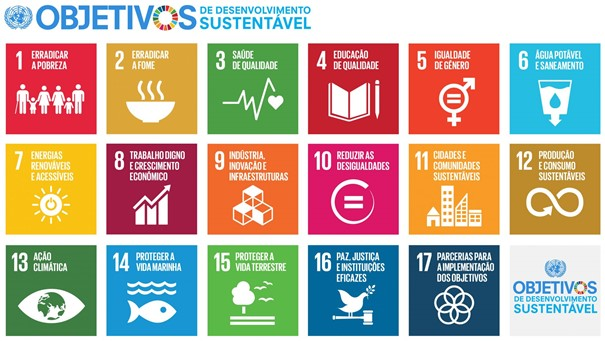
\includegraphics{Imagens/DesenvolvimentoSustentavel.jpg}
    \caption{Objectivos de Desenvolvimento Sustentável da ONU}
    \label{fig:ODS}
\end{figure}

\section{Objetivos e Perguntas de Pesquisa\label{se:objetivos}}

Foram aprovadas a nível europeu (2020)\cite{52020DC0299} sugestões de alterações aos serviços de sistema, que serão seguidas pelos Estados-Membros. Nesta dissertação, será realizada a aplicação dessas sugestões, identificando as melhorias em relação ao \textit{design} actual e avaliando se as novas sugestões serão suficientes para garantir a operação de um sistema elétrico \textasciitilde100\% renovável, potencialmente identificando ações adicionais para garantir a robustez e segurança do sistema elétrico sem o uso de combustíveis fósseis.\par
A penetração das \gls{vRES} no sistema de energia eléctrica trouxe maior incerteza na previsão em mercados de energia, pois estas estão mais sujeitos a elementos não controláveis como a velocidade do vento ou a radiação solar incidente.\par
As seguintes perguntas servirão de guia nesta pesquisa:\par

\begin{enumerate}[label=\alph*)]
  \item Podemos reduzir a incerteza na produção criada pela participação das \gls{vRES} nos sistemas de energia? 
  \item A alocação dinâmica pode ter um efeito positivo no mercado de reservas?
  \item É possível prever a necessidade de reserva necessária baixando a alocação desperdiçada?
\end{enumerate}

Para responder às perguntas \textit{supra} referidas, utilizaremos dados de previsão de geração de energia renovável para estimar a energia necessária para alocação secundária. Actualmente, os valores de previsão desse mercado estão distantes do consumo real, o que resulta em alocações no dia anterior que não estão em conformidade com as necessidades reais.\par
O objetivo deste trabalho é criar métodos de previsão para o dia seguinte, da necessidade de alocação de banda de reserva secundária, de modo a alocar banda suficiente e, simultaneamente, baixar a alocação em excesso, usando dados históricos das mesmas.\par
Iremos explorar a optimização da fórmula de alocação de banda de reserva da REN, testando novos valores para o parâmetro horário da mesma.\par
Utilizando técnicas de \textit{machine learning} vamos criar um modelo para a previsão de alocação necessária do dia seguinte.\par
Previsões mais exactas tornam possível uma melhor gestão das alocações, resultando num menor gasto de recursos energéticos e financeiros.\par

\section{Organização do Documento \label{se:organização}}

Este documento está dividido em capítulos. Sendo que os primeiros apresentam uma introdução às ideias e temas no 1, o estado de arte dos temas na literatura publicada, seguido de uma contextualização do tema do trabalho proposto no capítulo 2. Dentro da contextualização é de forma geral apresentado os mercados de energia, os sistemas de reserva, e os métodos de previsão para os mesmos, dentro destes o uso de fórmulas e o uso de \textit{machine learning}, formulando aqui a motivação e caminho de estudo.\par
No capítulo 3 apresentamos no sub-capítulo Ferramentas as bibliotecas criadas em \textit{python} para o presente estudo.
Segue o sub-capítulo Métodos onde abordamos os diferentes estudos presentes, como serão dirigidos e condições a alcançar. Dividindo o trabalho em estudos distintos para o tipo de previsões apresentadas no capítulo 2.
Métricas e Dados intitula o capítulo 4 que começa numa dissecção das métricas aplicadas ao longo das experiências e como estas influenciam a mesma, terminando num estudo geral dos dados utilizados, seus tratamentos e elações iniciais de análise. Apresentado também o que é usado como treino e como validação para as experiências.
No capítulo 5 são apresentados os resultados da experiência completa, incluindo as métricas apresentadas, apresentado gráficos de séries temporais das previsões conseguidas. Dando realce aos melhores modelos e optimizações conseguidos.
Termina com um breve capítulo conclusivo dando um pouco mais de contexto aos resultados, apresentando possíveis caminhos futuros de melhoria dos mesmos e discutindo o impacto de \textit{machine learning} no futuro das energias renováveis e consequentemente nos mercados de reserva.

% Os dois capítulos seguintes apresentam os dois diferentes estudos. No \hyperref[ch:estudo_1]{capítulo 4} é definido e apresentado o resultado do estudo da estimativa do parâmetro $\rho$ da fórmula de estimativa da \gls{REN}.\par
% No \hyperref[ch:estudo_2]{capítulo 5} explora-se o segundo estudo, o dimensionamento dinâmico da alocação necessária. São apresentados os dados utilizados com um estudo preliminar sobre os mesmos, e o tratamento necessário para usar nos modelos.\par
% No \hyperref[ch:ferramentas]{capítulo 6} as ferramentas de programação criadas para realizar a mesma.\par
% Os 3 capítulos seguintes são os descritivos da experiência em si. \hyperref[ch:metricas]{Capítulo 7} são as métricas usadas e criadas para a validação da experiência, \hyperref[ch:metodos]{capítulo 8} é a estrutura e parametrização da mesma, e \hyperref[ch:resultados_discussao]{capítulo 9} apresenta os resultados.\par
% Termina com um \hyperref[ch:conclusao]{capítulo conclusivo} onde são avaliadas as experiências como um todo, e o seu impacto no âmbito dos mercados de reserva.\par
\label{ch:intro}

% Revisão bibliográfica
\newpage
\thispagestyle{plain}
\chapter{Revisão bibliográfica}

A revisão bibliográfica deve recorrer a normas, livros, artigos científicos e, obrigatoriamente, deve indicar a bibliografia consultada de forma correta com recorrência a um reference manager. A maneira mais usual é adotar o sistema numerado por ordem de aparecimento do texto.\\
Isto é um exemplo de uma equação:

\begin{equation}
\label{eq:eq1}
    a = 1
\end{equation}

A tabela deve ter uma legenda por cima da mesma, tal como o exemplo em baixo. Se os valores da tabela não são calculados pelo autor e referem-se a valores de outros autores tem de constar as respetivas referências aos seus trabalhos.

%Tabela construida com https://www.tablesgenerator.com/

%Para ter a citação em formato [1] usem \cite{}
%Para usar citet ou citep teriam de modificar o style do \usepackage[backend=biber, natbib=true, style=numeric, sorting=none ]{biblatex} style de numerico para authoryear


\label{ch:revisao}

% Contextos
\newpage
\thispagestyle{plain}
\chapter{Contextos\label{ch:contextos}}

\section{Mercado de Serviços de Sistema \label{se:servicos_sistema}}
%\cite{Lopes2021}
%\cite{Watson1984}
%\citep{Schweppe1988}

O mercado de serviço de sistema é parte integrante dos mercados de energia e mantêm responsabilidade sobre a segurança do mesmo.\cite{dgegmss} \\
Serve para garantir o equilibrio entre a energia produzido e a consumida. Esta qualidade e segurança é controlada através da frequência e da potência activa, controlo de tensão e potência reactiva, arranque automático e outras técnicas de sistemas \cite{Rassid2017} \cite{Carneiro2016}. \\
Neste caso de estudo estamos interessados nos serviçoes de controlo de frequência. A nível europeu estes serviços são impostos pela ENTO-E (\textit{European Network of Transmission System Operators for Electricity}), e a operação dos mesmos é da responsabilidade dos TSO (\textit{Transmission System Operator} ou \textit{ Operador da Rede de Transporte}) nacionais.\\
Para manter o controlo de frequência o gestor de sistema deverá manter reservas para responder às diferenças entre a energia consumida e produzida na rede, que deve ser mantida em equilibrio. Quando o serviço de sistema precisa de actuar para manter a frequência no seu valor nominal, 50Hz na Europa, isto é feito alterando a potência activa dos geradores.  \\
Quando é necessário um aumento na potência chama-se a isto Banda de Reserva/Regulação a Subir, e quando é necessária uma diminuição chama-se à mesma a Descer. \\
Para isto, mo mercado ibérico, a tarefa é dividida em três reservas, primária, secundária e terciária. Esta divisão assenta no tempo de resposta que os sistemas precisam de ter, e na capacidade de actuação (MWh/Hz). \\

A reserva secundária, como sistema de segurança à reserva primária, regula-se pelo mercado de banda das reservas secundárias, que decorre no dia anterior ao que será necessário utilização da mesma. \\
Este valor alocado tem um custo para as operadoras, como tal a previsão do mesmo é importante para a gestão destes sistemas de segurança. Estas previsões são feitas através de estatiscas dos sistemas, e tendo em conta as areas de balanço que o mesmo têm. \\
Uma melhor previsão deste valor poderia levar a uma poupança, tanto financeira, como de recursos. \\

Estas previsões são feitas ao uso de formulas. Que por si só não preveêm a variabilidade dos sistemas de produção de energia renovável. Esta variabilidade sendo dificilmente previsivel, tem sido alvo de estudo com modelos de \textit{machine learning} \cite{} \\
Com bons resultados apresentados em estudo de energias renováveis, a aplicação dos mesmos metódos para as reservas de sistema parece um passo natural. \\



%\section{MIBEL \label{se:mibel}}
%\cite{Bessa2012}
%\cite{Carneiro2016}
%\cite{Fernandes2016}
%\citep{Agostini2021}

\label{ch:contexto}
% Dados

\newpage
\thispagestyle{plain}
\chapter{Estudo 1: Estimativa do parâmetro $\rho$ da fórmula da REN}



Para responder a primeira questão estudou-se o comportamento do parâmetro p na equação publicada pela REN para a Banda de Regulação Secundária a Subir:

\begin{equation} \label{eq:BRREN} 
    BR = \rho \times \sqrt{a \times  L_{max} + b^{2}} - b 
\end{equation}
onde:
\begin{itemize}
  \item $BR$: Banda de Reserva  de regulação secundária necessária (MW).
  \item $\rho$: Paramêtro horário.
  \item $a$ e $b$: Coeficientes empiricos, $a$=10MW e $b$=150MW .
  \item $L_{max}$: Pico máximo de consumo (MW).
\end{itemize}

Aqui queremos descobrir qual o valor do parâmetro $\rho$ (por hora do dia) que melhor nos descreve os dados reais. Para isso estudamos os valores reais usados para a Banda de Reserva, os valores resultantes da proposta de $\rho$  em \cite{Carneiro2016} e os valores resultados do estudo aqui proposto. Aproximar o parâmetro $\rho$  utilizando os dados históricos. \\
Todos os dados necessários são disponibilizados pelo operador do sistema no \href{https://mercado.ren.pt/PT/Electr}{site da REN}, com exceção do consumo máximo expectável. Este parâmetro é então substituído pelo consumo real, como uma aproximação à formulação indicada previamente.\\
Os dados estudados contêm entradas horárias desde 2010 até ao fim de 2018. Com as seguintes variáveis:\\

\begin{table}[H] \centering \caption{Dados REN} \begin{tabular}{ll}
\toprule
Variável & Unidades \\
\midrule
BANDA SUBIR & MW \\
BANDA DESCER & MW \\
Consumo real & MW \\
Consumo Máximo ENTSO-E & MW \\
\bottomrule
\end{tabular}
 \end{table}

Na equação \ref{eq:BRREN} BR equivale à soma de BANDA SUBIR e BANDA DESCER, onde aqui é sempre considerado que Banda a subir são $\frac{2}{3}$ da Banda de Reserva total e a Banda a descer é o restante $\frac{1}{3}$. \\
Aqui iremos aplicar o mapa de parâmetro $\rho$ apresentado em \cite{Carneiro2016} na formula \ref{eq:BRREN} para o cálculo da Banda de Reserva Carneiro2016 como benchmark. \\

\begin{table}[H] \centering \caption{Valores de $\rho$ apresentado em \cite{Carneiro2016}} \begin{tabular}{ll}
\toprule
Hora & $\rho$ \\
\midrule
1/2/8/9/24 & 1,6 \\
3/7/10/11/19/20 & 1,4 \\
4 & 1,3 \\
5/6/12/13/14/15/16/17/18/21/22/23 & 1,2 \\
\bottomrule
\end{tabular}
 \end{table}


Por outro lado, usando os dados de consumo real, calculamos o $\rho$ ideal para cada entrada, de onde estudamos a melhor normalização dos mesmos para cada hora. \\
O cálculo deste $\rho_{proposto}$ é apenas a utilização da fórmula \ref{eq:BRREN} mas em função de $\rho$ : \\

\begin{equation} \label{eq:rhoproposed} 
    \rho  = \frac{(BR + b)}{\sqrt{a \times L_max + b^{2}}}
\end{equation}


Arredondando o $\rho_{proposto}$ a uma casa decimal, podemos verificar que o histograma das diferentes propostas difere bastante. Sendo que esta apresenta uma curva de distribuição normal. \\


\begin{figure}[H]
    \centering
    \includegraphics[width=\textwidth]{plots/Histograma_parametro_p.png}
    \caption{Histograma $\rho$}
  \end{figure}


Olhando as distribuições por hora: \\

\begin{figure}[H]
    \centering
    \includegraphics[width=\textwidth]{plots/Valor_do_parametro_p_hora.png}
    \caption{Valor do paramêtro $\rho$ (hora)}
  \end{figure}

O $\rho_{proposto}$ apresenta um grande variabilidade em todas as horas, embora de notar que em todas tem um maior peso perto da mediana. O $\rho$ de comparação embora sempre dentro da distribuição note-se que cai quase sempre em zonas com pouco peso nestes dados históricos. \\
Calculamos $\rho$ possiveis para proposta final usando as seguintes aproximações: média, mediana, e média ponderada ao consumo, e à banda. \\

As distribuições por hora são as seguintes:

\begin{figure}[H]
    \centering
    \includegraphics[width=\textwidth]{plots/Comparação_de_p_propostos_por_hora.png}
    \caption{Histograma $\rho$}
\end{figure}

Todas seguem um percurso semelhante ao longo do dia, o qual também pode ser extrapolado para Carneiro2016. A média e mediana destacam-se seguindo muito parecidas, enquanto que as ponderadas também parecidas entre elas são bastante mais discretas. \\
Para a escolha da normalização deste parâmetro à Hora, estudou-se o erro entre a Banda Reserva calculada através das normalizações e a Banda Reserva disponível nos dados. \\


\begin{figure}[H]
    \centering
    \includegraphics[width=\textwidth]{plots/Comparação_das_metricas_de_Erro.png}
    \caption{Histograma $\rho$}
\end{figure}


\begin{table}[H]
    \caption{Erros de Banda de Reserva por método de normalização $rho$}    
    \resizebox{\linewidth}{!}{\begin{tabular}{lrrrr}
\toprule
 & MAE (MW) & RMSE (MW) & MedianAE (MW) & MAPE (\%)\\
Normalização &  &  &  &  \\
\midrule
Carneiro2016 & 53.07 & 66.54 & 44.53 & 18.70 \\
média & 30.94 & 39.19 & 25.38 & 11.58 \\
mediana & 30.85 & 39.20 & 25.17 & 11.51 \\
média ponderada banda & 32.15 & 40.61 & 26.45 & 12.19 \\
média ponderada consumo & 31.54 & 39.91 & 26.20 & 11.73 \\
\bottomrule
\end{tabular}
}
    \end{table}


A normalização com erros mais baixos é a mediana. Com um erro médio (de todo o histórico) para o consumo real de 11.51\% o que comparando com o benchmark de 18.70\% é uma melhoria  bastante considerável. \\
Comparando as bandas calculadas a uma média em cada hora: \\


\begin{figure}[H]
    \centering
    \includegraphics[width=\textwidth]{plots/média_historica_de_banda_de_reserva.png}
    \caption{Média historica de Banda de Reserva}
\end{figure}

Podemos ver que em termos de média horária, a Banda de Reserva calculada através do $\rho_{proposto}$ apresenta quase uma sobreposição por inteiro ao valor médio real. \\

Retiramos as médias dos erros percentuais e podemos observar: \\

\begin{figure}[H]
    \centering
    \includegraphics[width=\textwidth]{plots/erro_médio_por_hora_banda_de_reserva.png}
    \caption{Erro médio por hora Banda de Reserva}
\end{figure}

Em termos de média diária o erro pelo método proposto está bem abaixo da margem de erro do 5\% na banda, em todas as horas. E na outra tese apenas 10\% cai dentro dessa margem de erro. \\

Como tal o $\rho_{proposto}$ a partir do estudo dos dados  históricos é: \

\begin{table}[H] \centering \caption{Valores de $\rho$ propostos} \begin{tabular}{rr}
\toprule
Hora & $\rho$ \\
\midrule
1 & 1.621694 \\
2 & 1.576623 \\
3 & 1.486929 \\
4 & 1.364176 \\
5 & 1.313958 \\
6 & 1.318832 \\
7 & 1.504499 \\
8 & 1.612361 \\
9 & 1.638188 \\
10 & 1.613728 \\
11 & 1.601277 \\
12 & 1.485861 \\
13 & 1.451995 \\
14 & 1.457233 \\
15 & 1.440454 \\
16 & 1.421988 \\
17 & 1.424636 \\
18 & 1.420682 \\
19 & 1.553086 \\
20 & 1.588201 \\
21 & 1.480219 \\
22 & 1.478815 \\
23 & 1.474412 \\
24 & 1.635658 \\
\bottomrule
\end{tabular}
 \end{table}


% \begin{table}[H]
%     \caption{Valores de $\rho$ propostos}    
%     \resizebox{\linewidth}{!}{\begin{tabular}{rr}
\toprule
Hora & $\rho$ \\
\midrule
1 & 1.621694 \\
2 & 1.576623 \\
3 & 1.486929 \\
4 & 1.364176 \\
5 & 1.313958 \\
6 & 1.318832 \\
7 & 1.504499 \\
8 & 1.612361 \\
9 & 1.638188 \\
10 & 1.613728 \\
11 & 1.601277 \\
12 & 1.485861 \\
13 & 1.451995 \\
14 & 1.457233 \\
15 & 1.440454 \\
16 & 1.421988 \\
17 & 1.424636 \\
18 & 1.420682 \\
19 & 1.553086 \\
20 & 1.588201 \\
21 & 1.480219 \\
22 & 1.478815 \\
23 & 1.474412 \\
24 & 1.635658 \\
\bottomrule
\end{tabular}
}
%     \end{table}

Em relação a perdas por arredondamento, apresento o resultado dos erros por arrendamento em cada um da casas possíveis, concluindo que até à primeira casa decimal, pode ser feito arredondamento do parâmetro $\rho$, sem influenciar muito o erro: \\


\begin{figure}[H]
    \centering
    \includegraphics[width=\textwidth]{plots/Erro_médio_por_hora_Banda_de_Reserva_Arredondamento.png}
    \caption{Erro médio por hora Banda de Reserva (Arredondamento)}
\end{figure}



Neste estudo podemos comprovar que usando um $\rho$ extrapolado dos dados históricos, e um $L_{max}$ sendo o consumo real e não o consumo máximo calculado, os erros médios por hora ficam abaixo dos 5\%.\\ \label{ch:estudo_1}

\newpage
\thispagestyle{plain}
\part{Dimensionamento dinâmico da potência alocada na reserva secundária}

\chapter{Dados}
\section{Dados Utilizados\label{se:dadosestudo}}

Os dados em estudo são do mercado energético espanol, retirados do site da \href{https://www.esios.ree.es/es}{\gls{ESIOS}}.


\begin{table}[H]
    \caption{Indicadores retirados do site da ESIOS}    
    \resizebox{\linewidth}{!}{\csvautotabular{tabelas/indicators_metadata.csv}}
\end{table}


\subsection{Aquisição dos Dados}

No ambito da automatização destes dados foi modificado o repositorio \href{https://github.com/SanPen/\gls{ESIOS}}{\gls{ESIOS}} para ser usado como uma biblioteca de python, aberta, em pypi.\par
Sendo uma ferramenta mais facilmente acessivel para a extrair dados do mercado espanhol, \href{https://pypi.org/project/pyesios/}{pyesios}.\par
No âmbito de automatizar o processo, foram feitas contribuições a esta ferramenta para tornar mais acessível, e uma ferramenta aberta de python.\par


\thispagestyle{plain}

\section{Estudo dos dados}

Os dados que proponho a prever são os de Energia Usada na Banda de Reserva Secundária, tanto a subir como a descer: "UpwardUsedSecondaryReserveEnergy","DownwardUsedSecondaryReserveEnergy".\\



\begin{figure}[H]
  \centering
  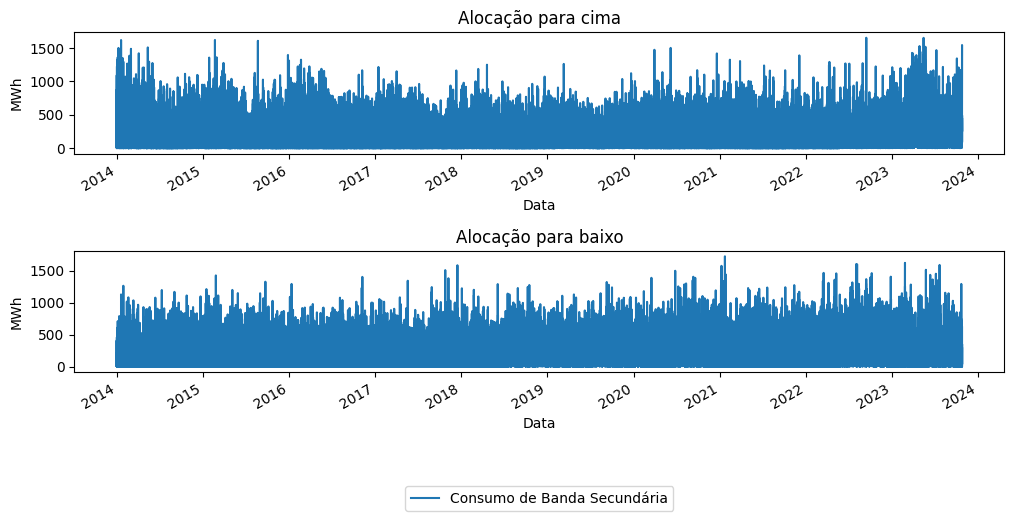
\includegraphics[width=\textwidth]{plots/consumo_originais.png}
  \caption{Serie Temporal dos dados alvo}
  \label{fig:targettimeseries}
\end{figure}


Para termos uma melhor percepção dos mesmos segue algumas janelas temporais mais pequenas.

\begin{figure}[H]
  \centering
  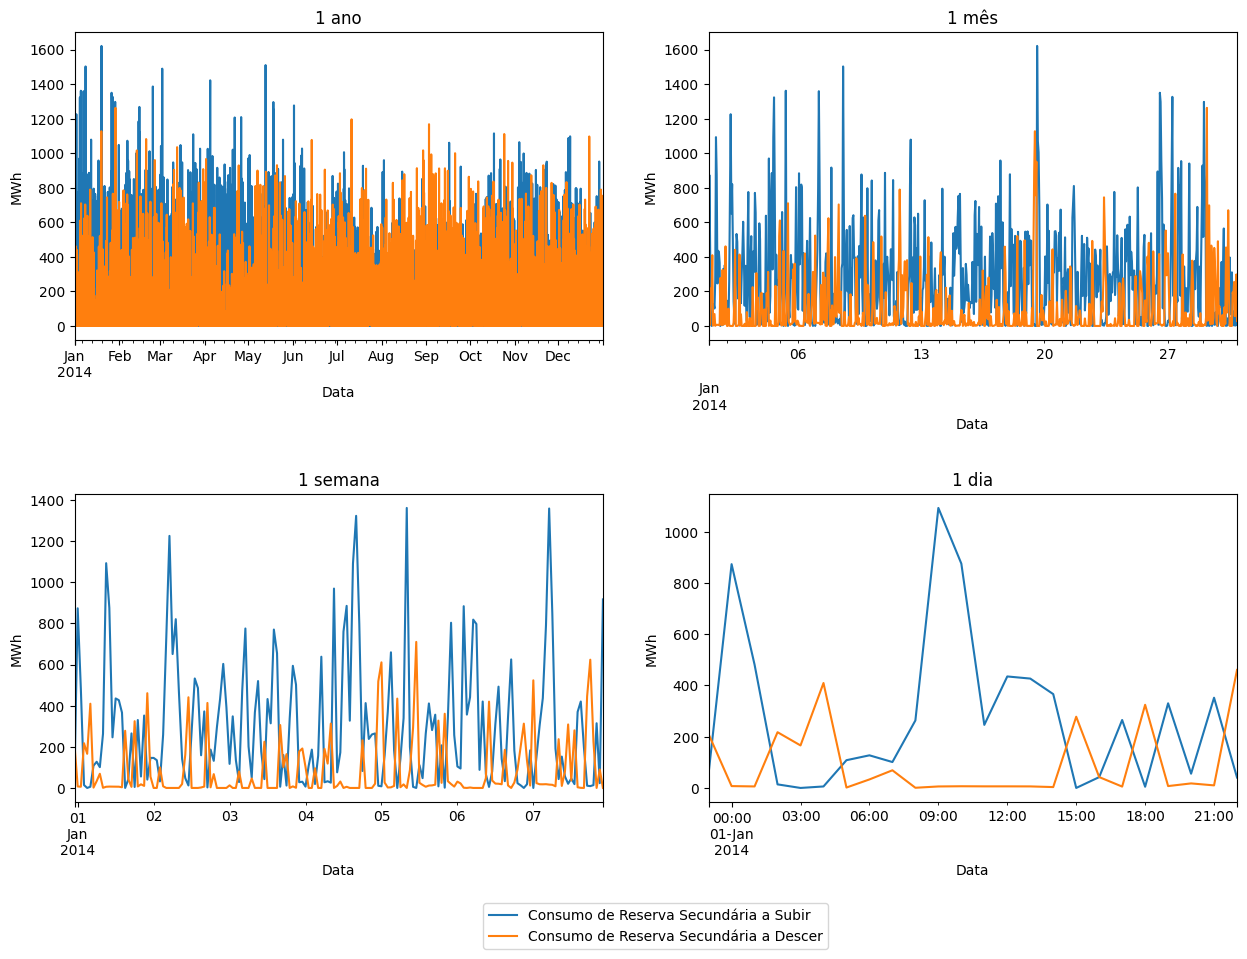
\includegraphics[width=\textwidth]{plots/target_timeseries_windows.png}
  \caption{Janelas Temporais dos dados alvo}
  \label{fig:targettimeserieswindows}
\end{figure}


Estas mostram claramente que ambos os atributos mantêm um comportamento tanto discreto, como linear, isto é, que ou existe algum valor, ou é zero, e se existe valor este tem comportamento linear.\\
A distribuição destes dados é claramente exponencial. O que é importante para a escolha de alguns parâmetros na modelação. \\

		
\begin{figure}[H]
  \centering
  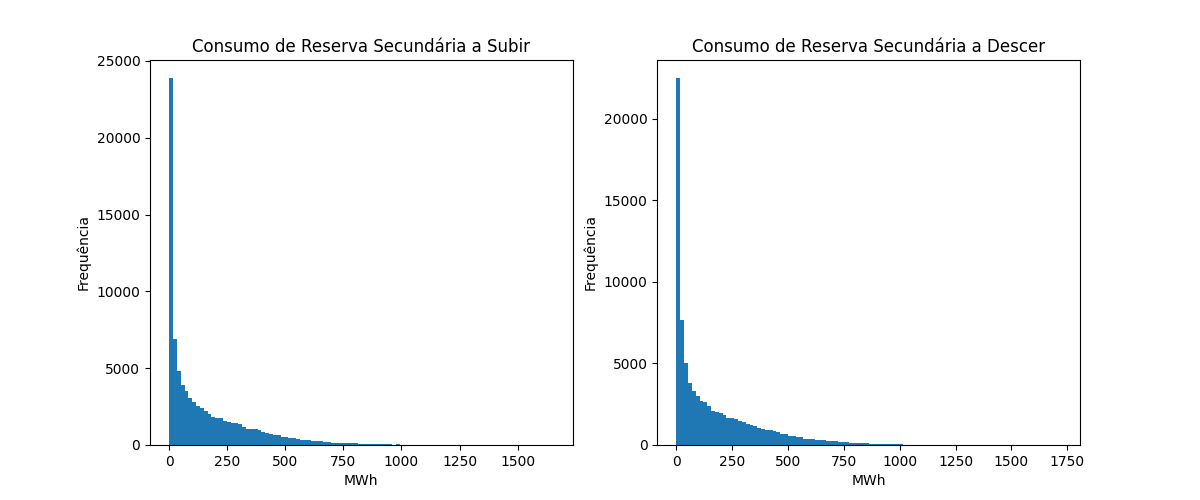
\includegraphics[width=\textwidth]{plots/target_histograms.png}
  \caption{Frequência dos dados alvos}
  \label{fig:targethistograms}
\end{figure}


\subsection{Correlações}

Os modelos vão depender bastante de correlação entre variáveis.

Nesta secção queremos tentar identificar se há visiveis relações entre as variáveis, e se há relações temporais  visiveis nas colunas alvo.


\subsubsection{Correlações entre atributos}


\begin{figure}[H]
  \centering
  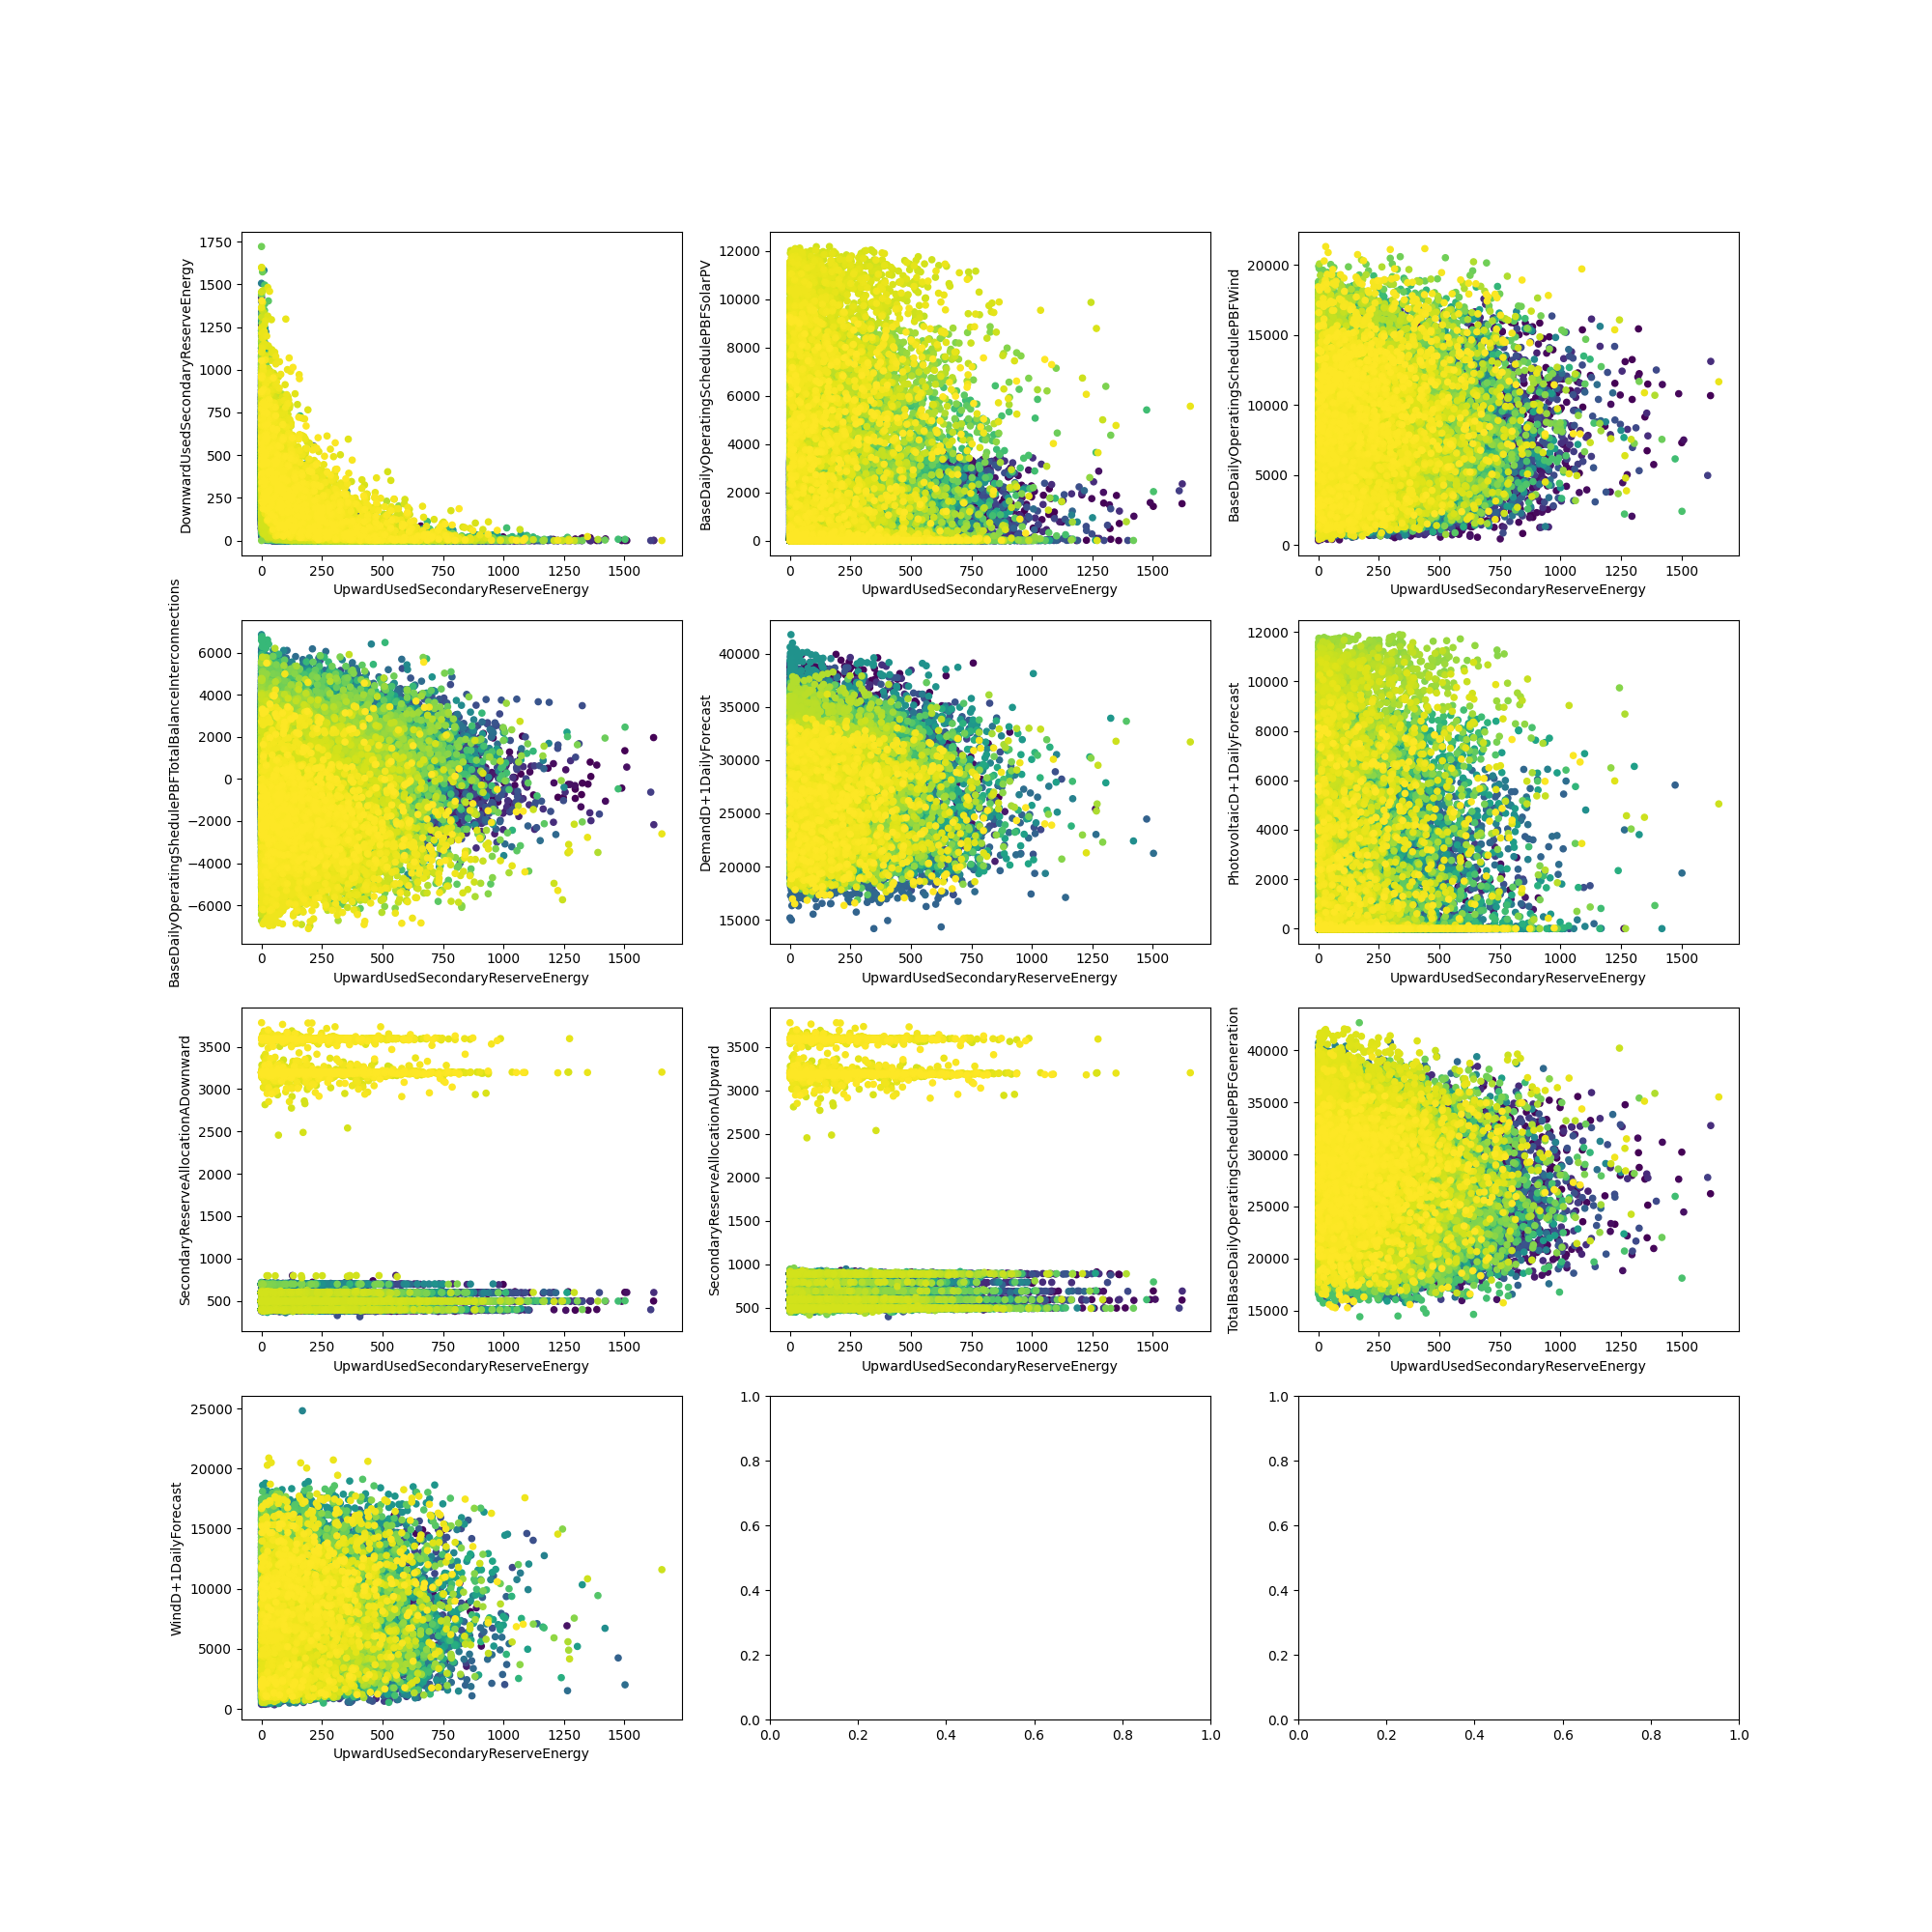
\includegraphics[width=\textwidth]{plots/feature_correlation.png}
  \caption{Correlação entre atributos}
  \label{fig:featurecorrelation}
\end{figure}

Esta figura apresenta a dispersão de valores entre a energia usada, primeiras três linhas a energia para cima e as seguintes a energia para baixo, e os outros atributos presentes.\\
As correlações entre variáveis parecem muitos escassas, o que apresenta já que a previsão destes dados usando estas variáveis vai ser um problema difícil.\\
Por norma é feito uma seleção de atributos baseado nestas correlações, eliminando assim os atributos que ajudam menos, ou até prejudicam os modelos.\\
Segue os valores de correlação onde podemos ver numericamente que existe muito pouca correlação entre os atributos. Onde a primeira coluna são os valores de correlação para a energia usada a subir e a segunda coluna as correlações da energia usada a descer.\\

\begin{figure}[H]
  \centering
  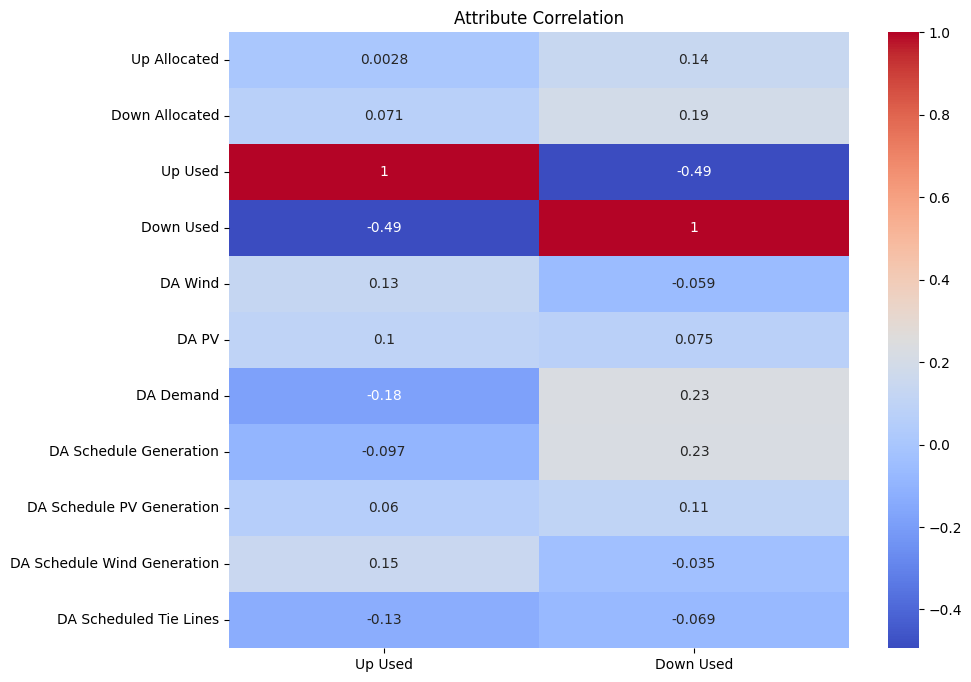
\includegraphics[width=\textwidth]{plots/correlation_heatmap.png}
  \caption{Valores de correlação entre atributos}
  \label{fig:correlationheatmap}
\end{figure}

\subsubsection{Correlações Temporais}

\begin{figure}[H]
  \centering
  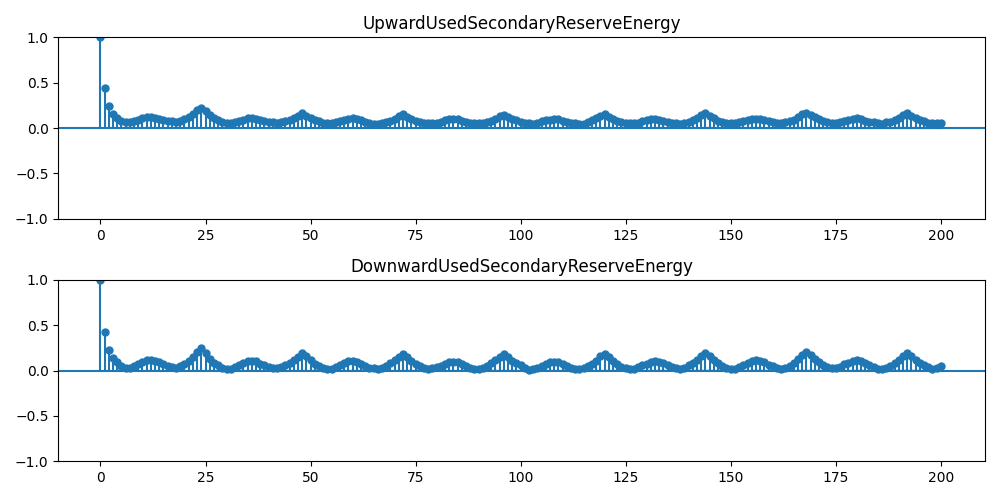
\includegraphics[width=\textwidth]{plots/autocorrelation.png}
  \caption{Autocorrelação Temporal}
  \label{fig:autocorrelation}
\end{figure}

A autocorrelação, em ambos os alvos, é mais forte nas 3 horas mais próximas, e nos pontos com diferença de 12 e 24 horas. \\
É de notar que estes valores são baixos, prometendo já também uma baixa regressividade temporal. \\
Os melhores saltos temporais e suas correlações são mostradas na tabelas em baixo:\\


\begin{table}[H]
  \caption{Autocorrelação Temporal}    
  \resizebox{\linewidth}{!}{\begin{tabular}{lllllllllll}
\toprule
\midrule
\multirow[t]{2}{*}{UpwardUsedSecondaryReserveEnergy} & horas & 1 & 2 & 24 & 23 & 25 & 168 & 144 & 192 & 48 \\
 & rácio & 0.44 & 0.24 & 0.22 & 0.19 & 0.19 & 0.17 & 0.16 & 0.16 & 0.16 \\
\cline{1-11}
\multirow[t]{2}{*}{DownwardUsedSecondaryReserveEnergy} & horas & 1 & 2 & 24 & 23 & 25 & 168 & 144 & 192 & 48 \\
 & rácio & 0.43 & 0.22 & 0.25 & 0.20 & 0.19 & 0.21 & 0.19 & 0.20 & 0.19 \\
\cline{1-11}
\bottomrule
\end{tabular}
}
  \label{tab:tempcorr}
  \end{table}

Outro ponto a denotar é que os objectos não têm um comportamento completamente linear, i.e., parece existir um comportamento discreto na questão ser alocado ou não esta reservas secundárias, e caso seja alocado, aí existir alguma linearidade. \\
Logo qualquer tipo de modelação terá de resolver primeiramente este problema. \\
Estas relações mostram que em termos de atributos usados vai ser um desafio complicado para qualquer tipo de modelo. \\
No âmbito desta dissertação queremos verificar a qualidade das previsões usando estes mesmo atributos, logo, não será feita seleção dos mesmos. \\
A nível da relação temporal, a maior parte dos modelos que iremos testar aplica um janela na dimensão temporal, usando todos os valores nessa janela, e aplicando os pesos nessas distâncias que mais se enquadram. Logo também não é relevante escolher apenas as distâncias temporais com maior correlação, pois os modelos vão fazer essa pesagem. \\


 \label{se:dadoscrus}



\thispagestyle{plain}



\section{Tratamento dos dados}

\textbf{Normalização} \par
A normalização foi deixada por ser aprendida nos modelos, sendo que todos têm como segunda camada, uma de normalização.\par

\textbf{Limpeza} \par

Podemos ver pelos gráficos seguintes que a existem alguns outliers, sendo estes definidos como 3 desvios padrão de distância à média.\par
Estes gráficos mostram também que existe uma variação do que são os valores normais de cada atributo a nível temporal. Logo um método de limpeza não se poderia basear apenas numa definição geral de outliers, mas teria de ser feito em janelas temporais.\par
Pelo mesmo argumento e visto que os outliers fazem parte do que queremos também descobrir, não é aplicada nenhum método de remoção dos mesmo, sendo os dados passados a cru para os modelos.\par


\begin{figure}[H]
  \centering
  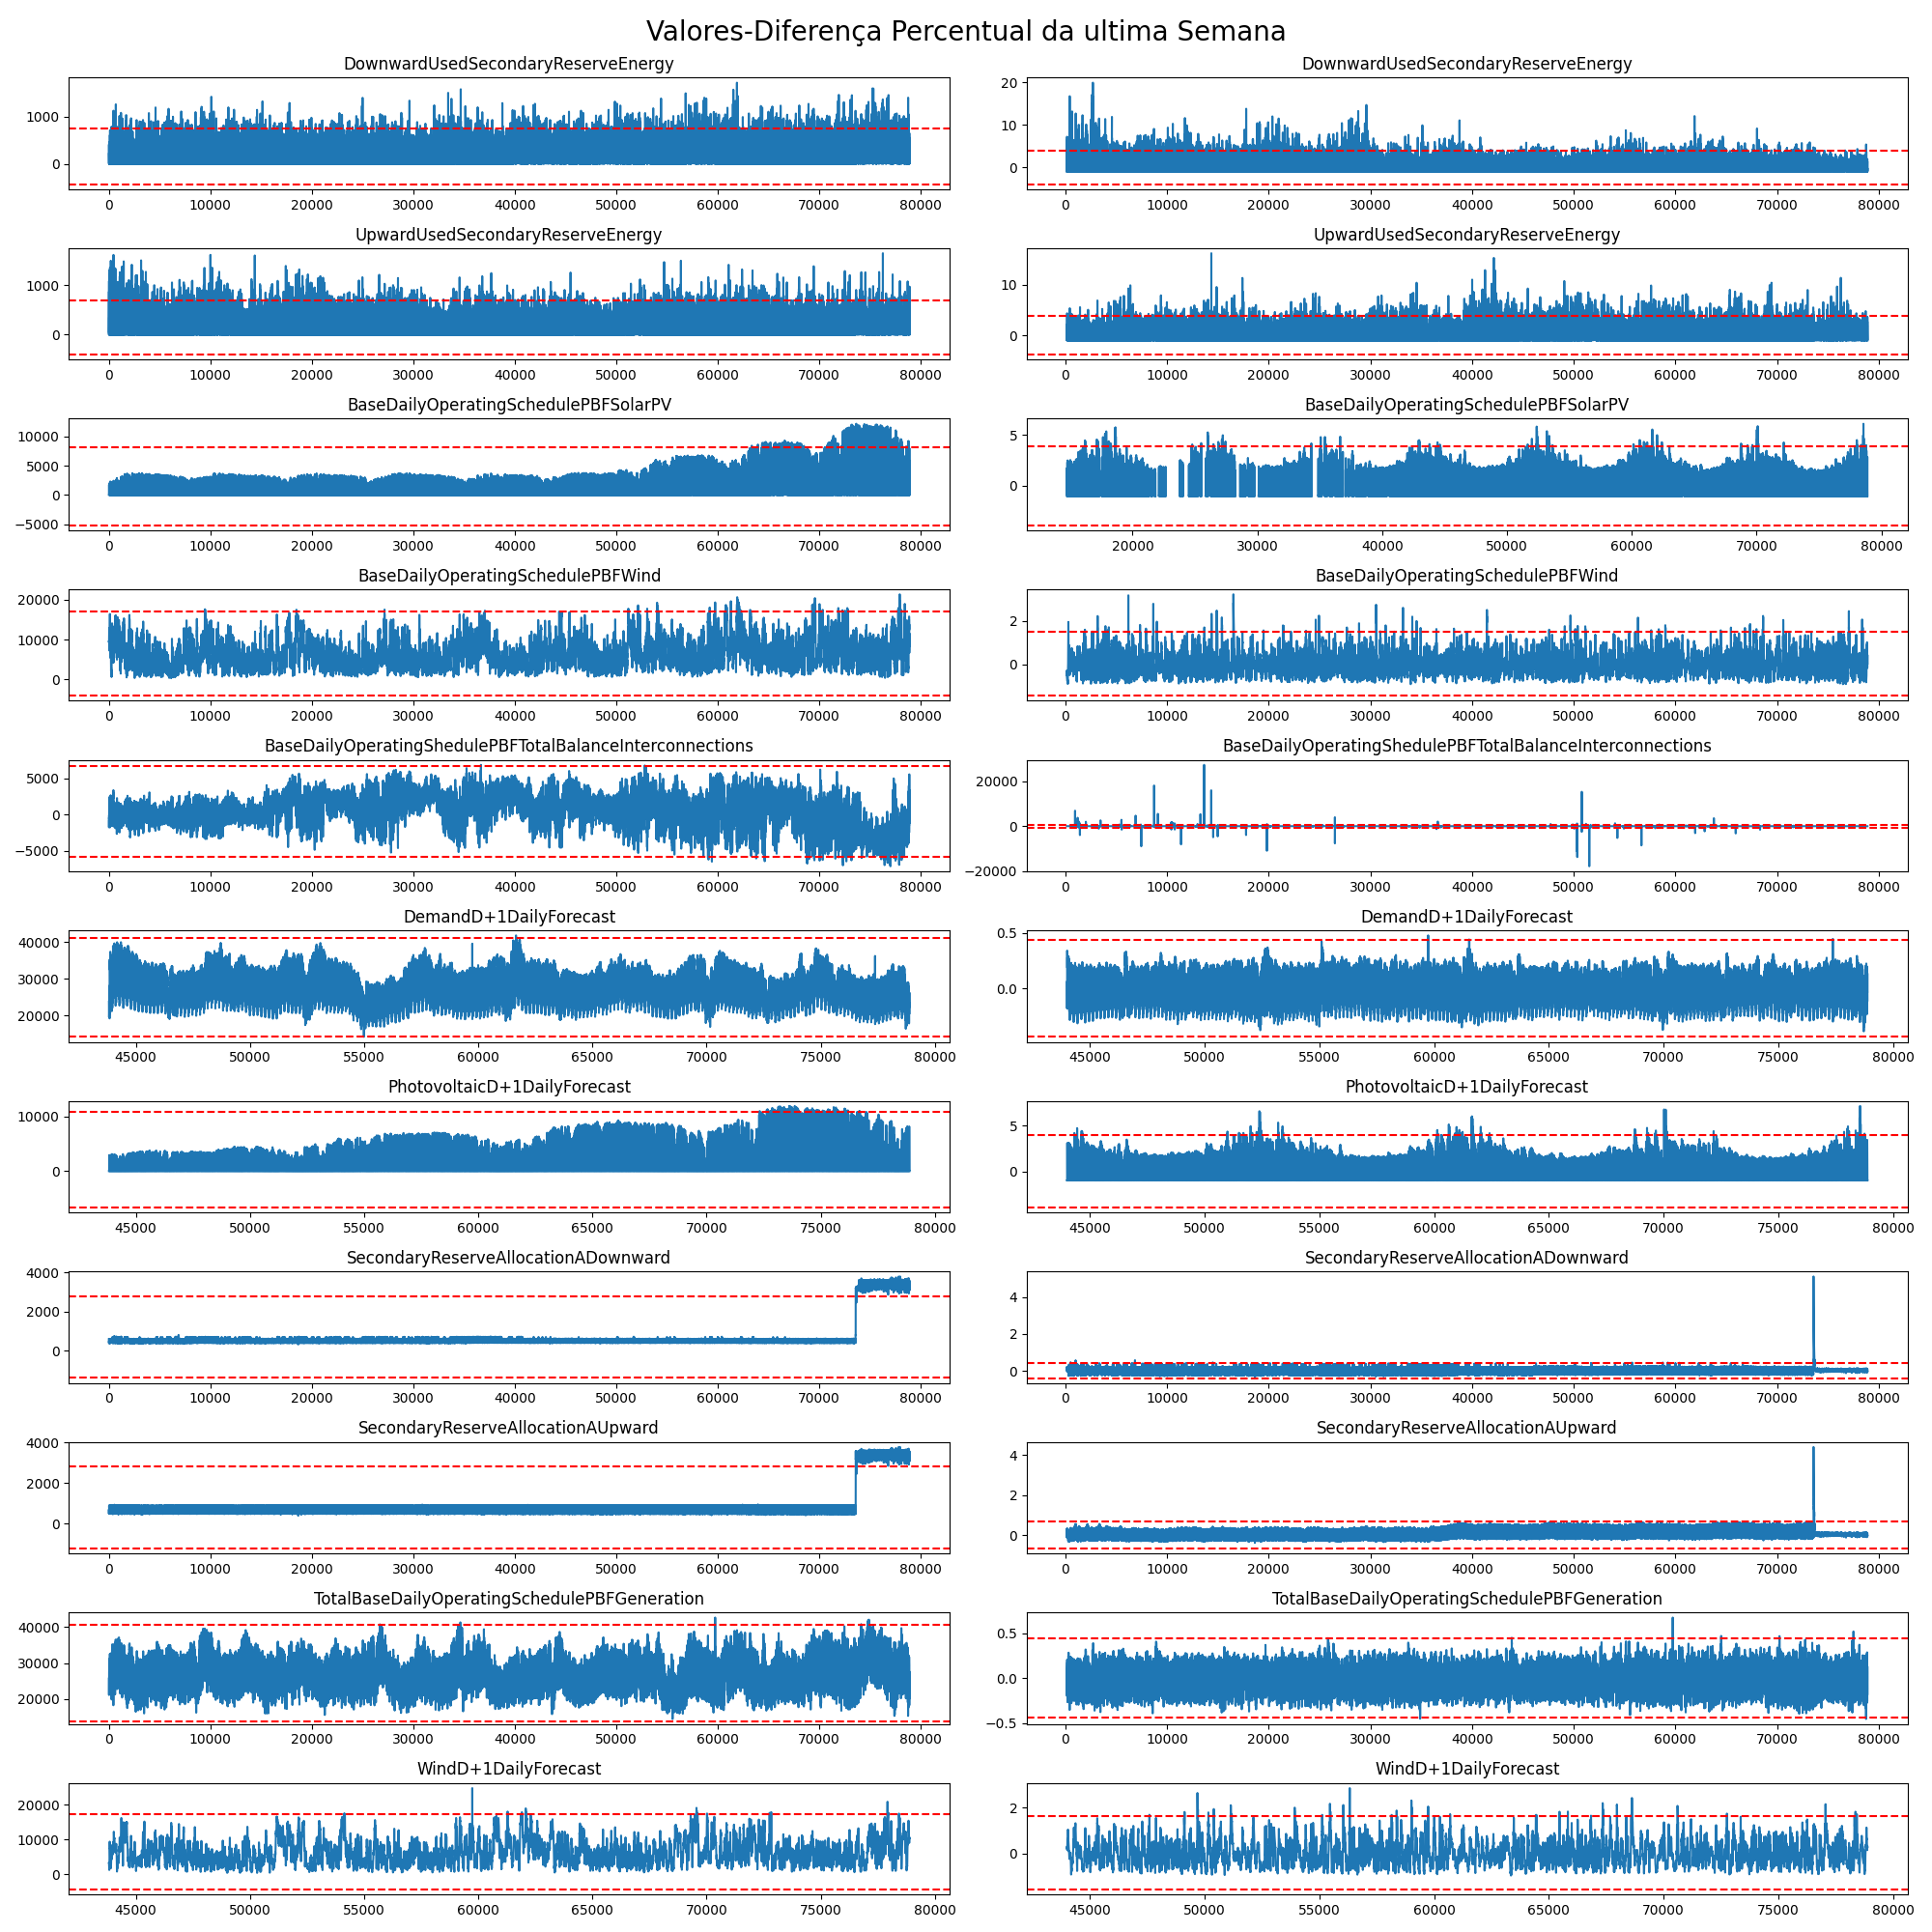
\includegraphics[width=\textwidth]{plots/Outliers_3stds.png}
  \caption{Outliers}
\end{figure}

Outra análise desta variação dos atributos a nível temporal leva-nos a que qualquer divisão dos dados para treino e teste deva levar as variações em consideração. Isto sendo que o treino deve ter representatividade de todas, ou maior parte, das condições diferentes.\par


\textbf{Dados em falta (Missing Data)}

Estudemos também o caso de dados em falta. Alguns destes atributos têm certas entradas vazias, e como podemos ver alguns não têm alguns anos inteiros.\par
Como queremos usar o máximo de dados possíveis iremos usar técnicas de imputing nesses dados.\par
Podemos ver que temos dados em falta de vários anos, em três atributos, e um tem algumas horas esporádicas em falta nos primeiros anos.\par

\begin{figure}[H]
  \centering
  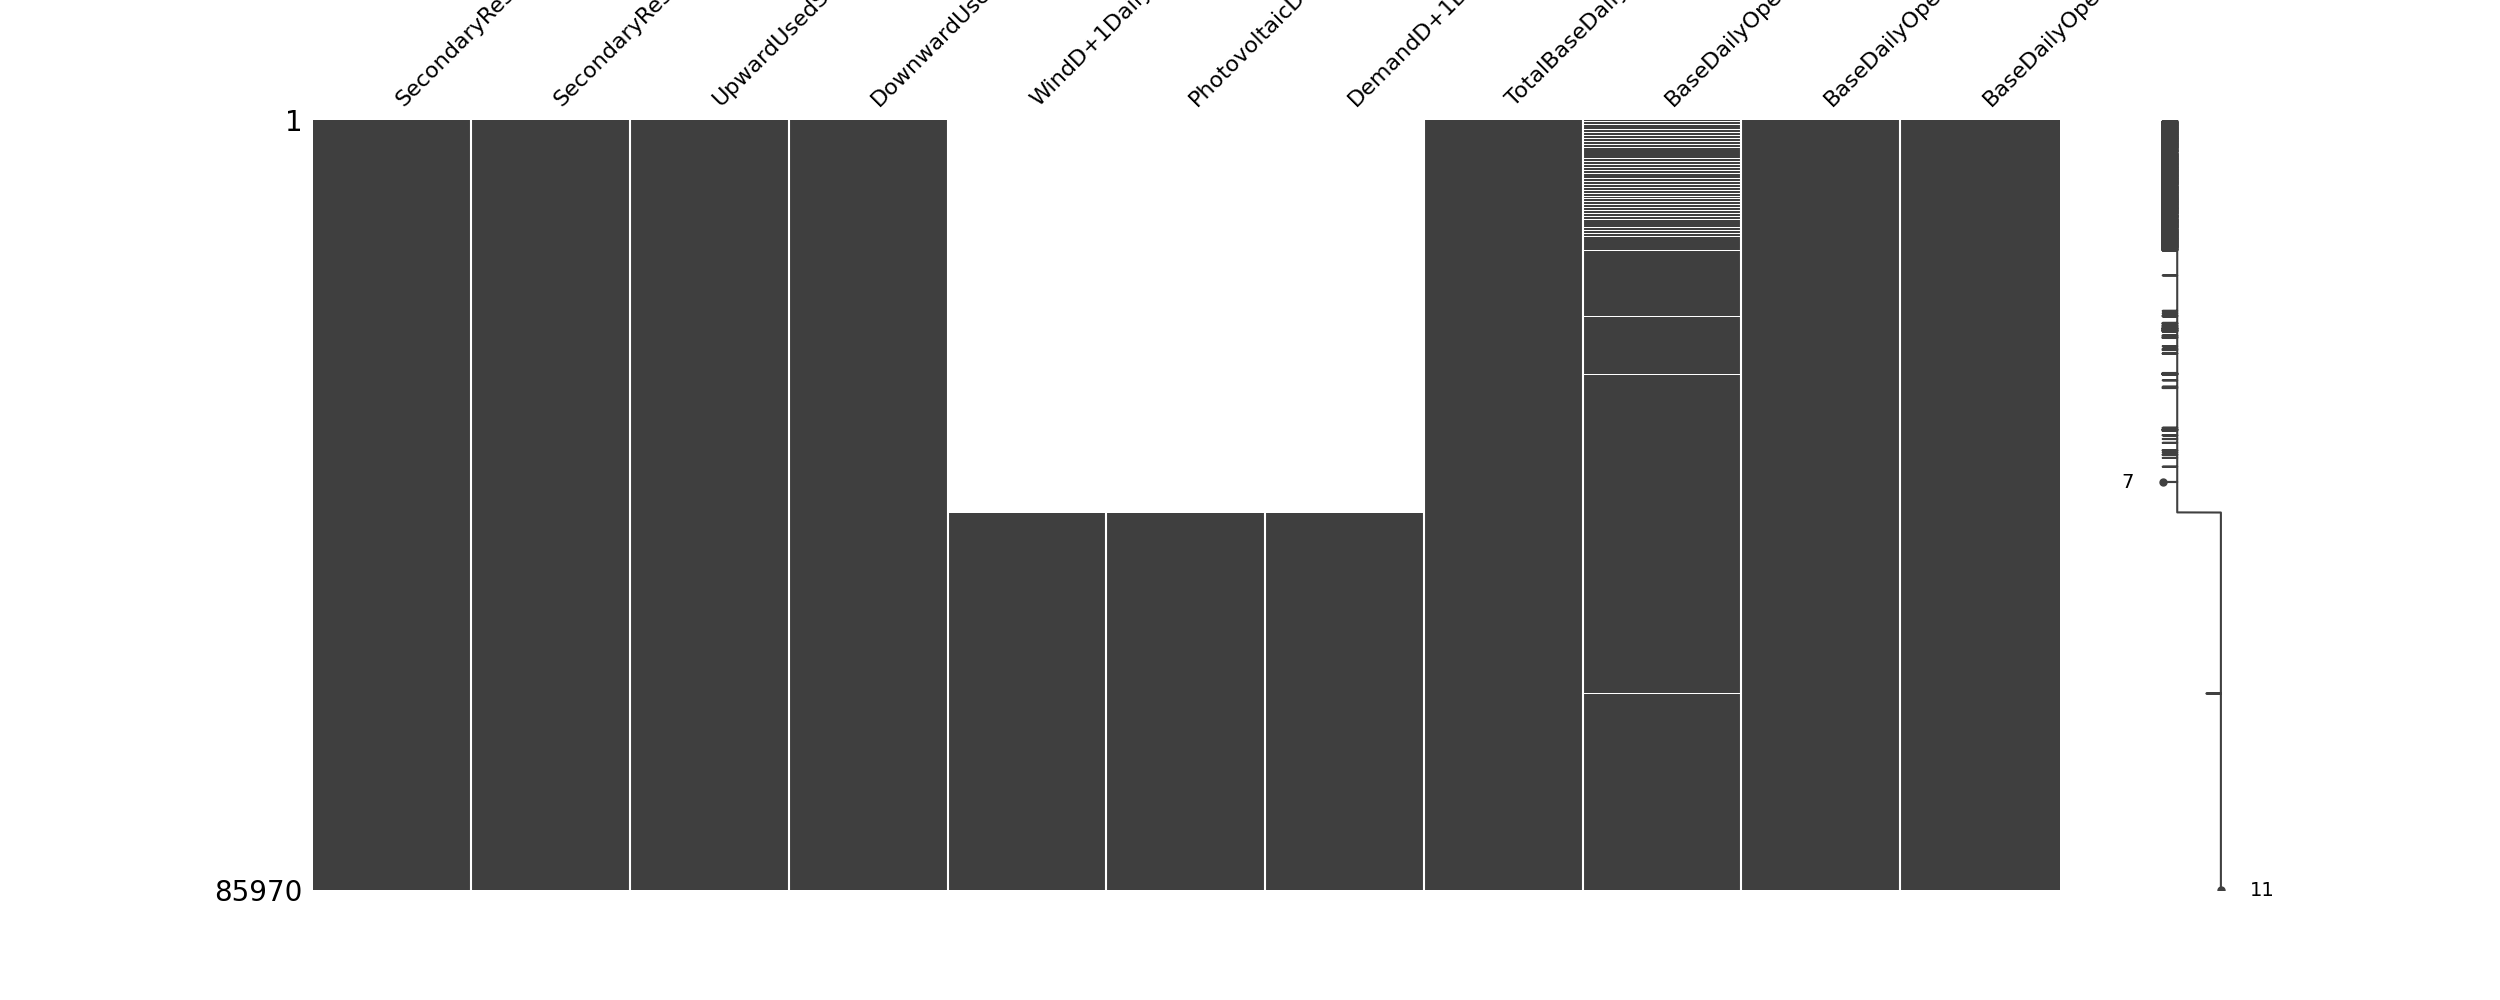
\includegraphics[width=\textwidth]{plots/missing_data.png}
  \caption{Dados em falta}
\end{figure}

Vamos aplicar o método experimental \href{https://scikit-learn.org/stable/modules/generated/sklearn.impute.IterativeImputer.html}{IterativeImputer} da biblioteca de python \href{https://scikit-learn.org/stable/index.html}{sklearn}.\par
Este metodo é baseado nos trabalhos de \cite{vanBuuren2011} e de \cite{Buck1960}.\par
Por ultimo foi adicionado ao dados mais atributos, sendo eles todos de cariz temporal. É adicionado atributos correspondentes à hora, ao dia do ano, ao dia da semana, ao dia do mês, mês, ano.\par

 \label{se:tratamentodados}

\subsection{Dados de treino}

Após o tratamento apresentado as estatísticas gerais dos dados usados para treinar o modelo são:

\begin{table}[H]
    \caption{Dados de Treino}    
    \resizebox{\linewidth}{!}{\begin{table}[H] 
    \caption{Training data summary. \label{training_data_sum}}
    \newcolumntype{C}{>{\centering\arraybackslash}X}
    \begin{tabularx}{\textwidth}{CCCCC}
    \toprule
    & \textbf{mean}	& \textbf{std}	& \textbf{min} & \textbf{max}\\
    \midrule
    Down Used & 168.20 & 199.67 & 0.00 & 1721.40 \\
    Up Allocated & 662.94 & 150.62 & 399.00 & 958.00 \\
    Down Allocated & 549.27 & 126.67 & 312.00 & 956.00 \\
    Up Used & 158.10 & 191.62 & 0.00 & 1654.80 \\
    DA Wind & 5824.12 & 3413.15 & 71.33 & 20879.30 \\
    DA PV & 1666.31 & 2719.60 & 0.00 & 14925.30 \\
    DA Demand & 27944.24 & 4479.39 & 14170.00 & 41773.00 \\
    DA Schedule Generation & 27249.43 & 4603.58 & 13470.50 & 42707.60 \\
    DA Schedule PV Generation & 1714.09 & 2815.35 & 0.00 & 16358.90 \\
    DA Schedule Wind Generation & 6525.51 & 3582.36 & 308.60 & 21619.60 \\
    DA Scheduled Tie Lines & 290.58 & 2157.11 & -7817.00 & 6858.50 \\
    \bottomrule
    \end{tabularx}
    % \noindent{\footnotesize{\textsuperscript{1} Tables may have a footer.}}
\end{table}

}
    \end{table}
 \label{ch:estudo_2}


% Arquiteturas a estudar
% \newpage
% \thispagestyle{plain}
% \chapter{Arquitecturas de Modelos\label{ch:arquiteturas_modelos}}

Grande parte da literatura sobre previsões em modelos de apredizagem apresenta as mesmas arquiteturas, sendo que são depois aprimoradas consoate os dados e o problema. \\
Apresento aqui as arquitecturas mais usadas em previsões, como também algumas usadas noutros ramos tentado prever a compatibilidade neste problema. \\
% TODO: meter citaçao para o uso de cada uma em previsões
Neste trabalho vamos usar arquiteturas de FCNN (Fully Connected Neural Network), CNN (Convolutional Neural Networks), LSTM (Long Short-Term Memory) e Transformer.\\




\section{FCNN\label{se:fcnn_sec}}

A arquitetura mais simples FCNN, Redes Neuronais Totalmente Conectadas , é constituída por camadas em que cada neurónio está ligado a todos os neurónios da camada seguinte. Isto significa que cada caraterística de entrada tem um peso associado, e esses pesos são aprendidos durante o treino. A saída de cada neurónio é calculada através da aplicação de uma função de ativação à soma ponderada das suas entradas.\\
Cada neurónio gera uma operação, inicialmente aleatória, para tentar reproduzir uma função que traduza a entrada na saída ideal.\\
Esta arquitectura tem como base o Perceptão inicialmente proposto em \cite{Rosenblatt1958}. Este apresentava um Perceptão que fazia uma decisão binária baseado nas somas pesadas de todas as entradas.\\
A ideia é a base utilizada actualmente, mas apresentava algumas limitações, e muita computação, o proposto por \cite{Minsky1969}, eleva a ideia com a introdução da função de activação e o bias. A utilização mais recorrente actual é a proposta em \cite{Haykin1999}.


\begin{figure}[H]
	\centering
	\resizebox{\linewidth}{!}{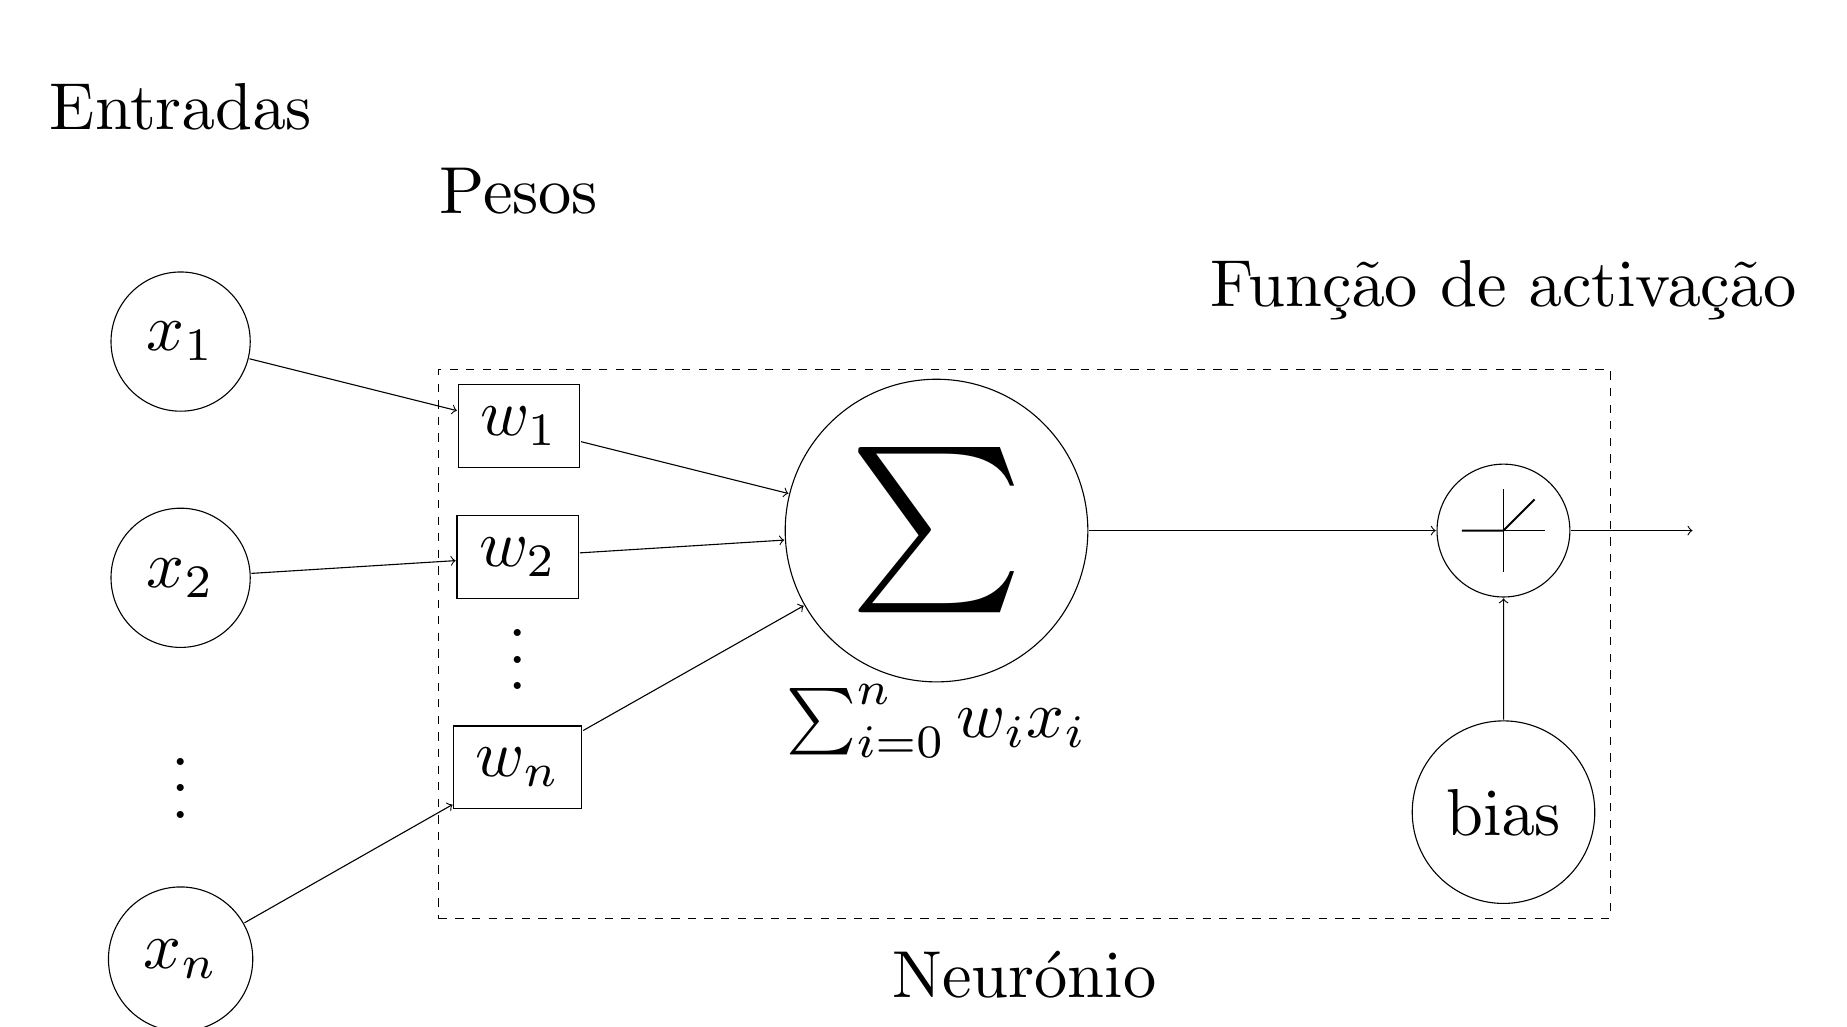
\begin{tikzpicture}[scale=2.4, transform shape]
    % Draw input nodes
    \foreach \h [count=\hi ] in {$x_2$,$x_1$}{%
          \node[input] (f\hi) at (0,\hi*1.25cm-1.5 cm) {\h};
        }
    % Dot dot dot ... x_n
    \node[below=0.62cm] (idots) at (f1) {\vdots};
    \node[input, below=0.62cm] (last_input) at (idots) {$x_n$};
    % Draw summation node
    \node[functions] (sum) at (4,0) {\Huge$\sum$};
    \node[below=0.69cm] at (sum) {$\sum_{i=0}^n w_ix_i$};
    % Draw edges from input nodes to summation node
    \foreach \h [count=\hi ] in {$w_2$,$w_1$}{%
          \path (f\hi) -- node[weights] (w\hi) {\h} (sum);
          \draw[->] (f\hi) -- (w\hi);
          \draw[->] (w\hi) -- (sum);
        }
    % Dot dot dot ... w_n
    \node[below=0.05cm] (wdots) at (w1) {\vdots};
    \node[weights, below=0.45cm] (last_weight) at (wdots) {$w_n$};
    % Add edges for last node and last weight etc
    \path[draw,->] (last_input) -- (last_weight);
    \path[draw,->] (last_weight) -- (sum);
    % Draw node for activation function
    \node[functions] (activation) at (7,0) {};
    \node[small_input, below=1cm] (bias) at (activation) {bias};
    \path[draw,->] (bias) -- (activation);

    % Place activation function in its node
    \begin{scope}[xshift=7cm,scale=1.25]
        \addaxes
        % flexible selection of activation function
        \relu
        % \stepfunc
    \end{scope}
    % Connect sum to relu
    \draw[->] (sum) -- (activation);
    \draw[->] (activation) -- ++(1,0);
    % Labels
    \node[above=1cm]  at (f2) {Entradas};
    \node[above=1cm] at (w2) {Pesos};
    \node[above=1cm] at (activation) {Função de activação};

    % Neuron
    \node[draw, dashed, fit= (w2) (last_weight) (activation) (bias), inner sep=0.5em] (square){};
    \node[below=1.5cm] at (square) {Neurónio};

\end{tikzpicture}}
	\caption{Ilustração de um neurónio. Adaptado de \cite{Haykin1999}}
	\label{fig:neuronio}
\end{figure}



\section{CNN\label{se:cnn_sec}}
% TODO: add cites do conv 
As Redes Neuronais Convolucionais (CNN) diferem das FCNN no sentido em que os filtros (neurónios) não são criados aleatoriamente, mas sim cada filtro trata de uma parte da camada de entrada. Nas convoluções é criada uma janela móvel que percorre a camada, criando um saída desse conjunto de pontos. Esta janela move-se sempre subsequentemente.\\
Esta operação é normalmente feita na dimensão (ou dimensões) em que queremos perceber padrões.\
Nos nossos dados a convolução será na dimensão temporal.\\
Se tivermos uma matriz com nove passos temporais (N,9,1), se o tamanho da janela de convolução for 3, teremos uma saída de tamanho 6 (N, 6, 1).\\
\begin{figure}[H]
	\centering
	\resizebox{\linewidth}{!}{
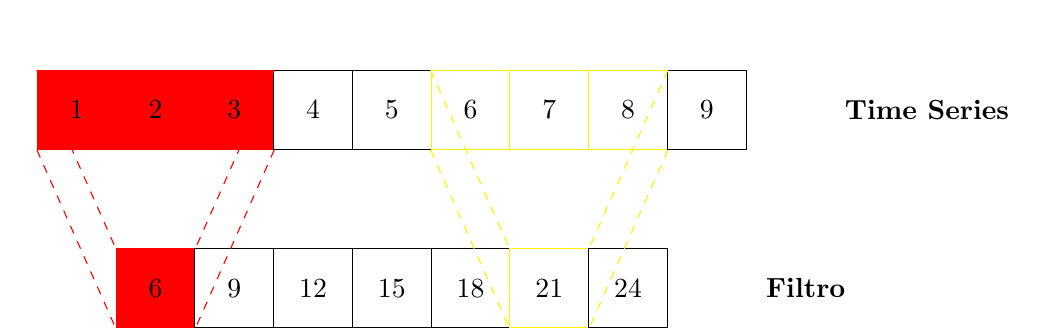
\begin{tikzpicture}
    % Time series
    \matrix (M1) [matrix of math nodes, nodes={draw, minimum size=1cm, anchor=center}, 
    column sep=-\pgflinewidth, row sep=-\pgflinewidth,
    ] {
        \node[fill=red, draw=red] (M1-1-1) {1}; & \node[fill=red, draw=red] (M1-2-1) {2};
        & \node[fill=red, draw=red] (M1-3-1) {3}; &
        4 & 5 & \node[draw=yellow] (M1-6-1) {6}; & \node[draw=yellow] (M1-7-1) {7};
        & \node[draw=yellow] (M1-8-1) {8}; & 9 \\
    };
    
    % Kernel
    \matrix (M2) [below=of M1, matrix of math nodes, nodes={draw, minimum size=1cm, anchor=center}, 
    column sep=-\pgflinewidth, row sep=-\pgflinewidth,
    ] {
        \node[fill=red, draw=red] (M2-1-1) {6}; & 9 & 12 & 15 & 18 & \node[draw=yellow] (M2-5-1) {21}; & 24 \\
    };

    \draw[dashed, red] (M1-1-1.north west) -- (M2-1-1.north west);
    \draw[dashed, red] (M1-3-1.north east) -- (M2-1-1.north east);
    \draw[dashed, red] (M1-1-1.south west) -- (M2-1-1.south west);
    \draw[dashed, red] (M1-3-1.south east) -- (M2-1-1.south east);

    \draw[dashed, yellow] (M1-6-1.north west) -- (M2-5-1.north west);
    \draw[dashed, yellow] (M1-8-1.north east) -- (M2-5-1.north east);
    \draw[dashed, yellow] (M1-6-1.south west) -- (M2-5-1.south west);
    \draw[dashed, yellow] (M1-8-1.south east) -- (M2-5-1.south east);

    
    % Titles
    \node [right=1cm, align=center, font=\bfseries] at (M1.east) {Time Series};
    \node [right=1cm, align=center, font=\bfseries] at (M2.east) {Filtro};
    \end{tikzpicture}}
	\caption{Ilustração da operação de Convolução}
	\label{fig:conv_layer1D}
\end{figure}

Anteriormente ignoramos o número de filtros. Mas as convoluções criam o número pedido de filtros para cada janela temporal. Aqui cada filtro vai funcionar como na camada FCNN, onde cada um começa com uma operação pseudo aleatória. Esta operação normalmente é feita na dimensão dos atributos.\\
Ou seja, a quantidade de filtros que esta camada irá produzir por convolução.\\
Se tivermos a mesma entrada que anteriormente mas com 4 atributos (N, 9, 4), e se definir o número de filtros para 2 teremos uma saída (N, 6, 2).\\
Ou seja, dois filtros por cada janela temporal.\\


\begin{figure}[H]
	\centering
	\resizebox{\linewidth}{!}{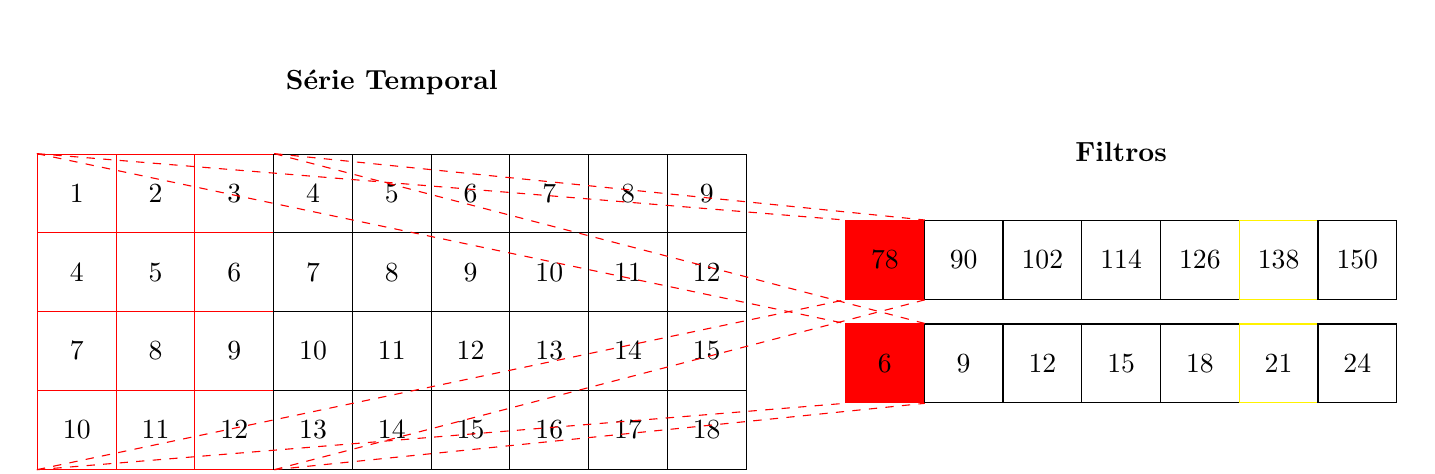
\begin{tikzpicture}[scale=2]
    \matrix (M1) [matrix of math nodes, nodes={draw, minimum size=1cm, anchor=center}, 
    column sep=-\pgflinewidth, row sep=-\pgflinewidth,]
{
    \node[draw=red] (M1-1-1) {1}; & \node[draw=red] (M1-1-2) {2}; & \node[draw=red] (M1-1-3) {3}; & 4 & 5 & 6 & 7 & 8 & 9\\
    \node[draw=red] (M1-2-1) {4}; & \node[draw=red] (M1-2-2) {5}; & \node[draw=red] (M1-2-3) {6}; & 7 & 8 & 9 & 10 & 11 & 12\\
    \node[draw=red] (M1-3-1) {7}; & \node[draw=red] (M1-3-2) {8}; & \node[draw=red] (M1-3-3) {9}; & 10 & 11 & 12 & 13 & 14 & 15\\
\node[draw=red] (M1-4-1) {10}; & \node[draw=red] (M1-4-2) {11};
& \node[draw=red] (M1-4-3) {12}; & 13 & 14 & 15 & 16 & 17 & 18\\
};

\matrix (M2) [matrix of math nodes, nodes={draw, minimum size=1cm, anchor=center}, 
column sep=-\pgflinewidth, row sep=0.3cm,
    right=of M1]
{
    \node[fill=red, draw=red] (M2-1-1) {78}; & 90 & 102 & 114 & 126 & \node[draw=yellow] (M2-1-5) {138}; & 150 \\
    \node[fill=red, draw=red] (M2-2-1) {6}; & 9 & 12 & 15 & 18 & \node[draw=yellow] (M2-2-5) {21}; & 24 \\
    };

% Titles
\node [above=0.5cm, align=center, font=\bfseries] at (M1.north) {Série Temporal};
\node [above=0.5cm, align=center, font=\bfseries] at (M2.north) {Filtros};
 
\draw[dashed, red] (M1-1-1.north west) -- (M2-1-1.north west);
\draw[dashed, red] (M1-1-1.north west) -- (M2-2-1.north west);

\draw[dashed, red] (M1-1-3.north east) -- (M2-1-1.north east);
\draw[dashed, red] (M1-1-3.north east) -- (M2-2-1.north east);

\draw[dashed, red] (M1-4-1.south west) -- (M2-1-1.south west);
\draw[dashed, red] (M1-4-1.south west) -- (M2-2-1.south west);


\draw[dashed, red] (M1-4-3.south east) -- (M2-1-1.south east);
\draw[dashed, red] (M1-4-3.south east) -- (M2-2-1.south east);



% TODO: add legenda em pequeno
%\node [right=1cm, align=center, font=\bfseries] at (matrix1.west) {Atributos};
%\node [right=1cm, align=center, font=\bfseries] at (matrix1.south) {tempo};


\end{tikzpicture}}
	\caption{Ilustração da camada de Convolução}
	\label{fig:conv_layer}
\end{figure}

As convoluções podem realizar as operações em mais dimensões, é comum usar 2D para imagens, e 3D para vídeos. Neste trabalho apenas trabalhamos com convoluções 1D.\\

\subsection{UNET\label{se:unet_sec}}

Um desenho especial de CNN, normalmente usando em modelação de imagens, e primeiro proposto em \cite{Shelhamer2014}, a arquitectura UNET passa por criar uma rede de expansão dos filtros, usando convoluções, e de seguida uma rede de contracção dos mesmo, até aos tamanhos pretendidos.\\
Nas suas ligações UNET junta informação de filtros passados (não de nível temporal mas de rede neuronal) para realçar informação já trabalhada, e assim identificar padrões de vários contextos diferentes.\\
É chamada assim pois é uma rede (NET) que forma um U na sua expansão, contracção e ligações entre estes.\\
Em cada camada de encoding vai usando convulucões para criar novos filtros e diminuir a dimensionalidade, enquanto que na fase de decoding vai usar convoluções para aumentar a dimensionalidade e diminuir o número de filtros, adicionando a camada decoder de tamanho análogo.\\

\begin{figure}[H]
	\centering
	\resizebox{\linewidth}{!}{\begin{tikzpicture}[ node distance = 2cm, auto, block/.style={ rectangle, draw, align=center, minimum width=2cm, minimum height=1cm }, line/.style={ draw, -latex' } ]
    % Encoder (Contracting Path)
    \node [block] (input) {Input};
    \node [block, below right=of input, xshift=-2cm] (enclayer1) {Enconding1};
    \node [block, below right=of enclayer1, xshift=-1.8cm] (enclayer2) {Enconding2};
    \node [block, below right=of enclayer2, xshift=-1.6cm] (enclayer3) {Enconding3};
    % (None, 168, 18) 
    
    \node [block, below right=of enclayer3] (up1) {Enconding4};
    
    % Decoder (Expanding Path)
    \node [block, above right=of up1] (declayer1) {Decoding1};
    \node [block, above right=of declayer1, xshift=-1.6cm] (declayer2) {Decoding2};
    \node [block, above right=of declayer2, xshift=-1.8cm] (declayer3) {Decoding3};
    \node [block, above right=of declayer3, xshift=-2cm] (output) {Output};
    
    % Skip Connection
    % \draw [line] (pool1) -- ++(0,-1) -| (up1);
    
    % Connections
    \draw [line] (input) -- (enclayer1);
    \draw [line] (enclayer1) -- (enclayer2);
    \draw [line] (enclayer2) -- (enclayer3);
    \draw [line] (enclayer3) -- (up1);
    \draw [line] (up1) -- (declayer1);
    
    
    \draw [line] (declayer1) -- (declayer2);
    \draw [line] (declayer2) -- (declayer3);
    \draw [line] (declayer3) -- (output);
    
    
    \draw [line] (input) -- (output);
    \draw [line] (enclayer1) -- (declayer3);
    \draw [line] (enclayer2) -- (declayer2);
    \draw [line] (enclayer3) -- (declayer1);
    
    
    \end{tikzpicture}}
	\caption{Ilustração uma rede UNET.}
	\label{fig:unet_graph}
\end{figure}


\section{RNN\label{se:rnn_sec}}

As Redes Neuronais Recorrentes (RNN) são projetadas para processar sequências de dados, onde a ordem dos elementos é importante. Elas funcionam passando informações de um neurónio para outro em uma cadeia, o que permite que cada neurónio seja influenciado pelo estado anterior da rede.\\
Isso é feito através de loops internos que permitem à rede "lembrar" informações de etapas anteriores. No entanto, as RNNs enfrentam dificuldades ao tentar lembrar informações de longo prazo, devido ao problema conhecido como desvanecimento do gradiente, onde os gradientes se tornam muito pequenos e impedem a atualização eficaz dos pesos da rede.\\

\subsection{LSTM\label{se:lstms_sec}}

As redes Long Short-Term Memory (LSTM) são um tipo especial de RNN projetado para superar os problemas de memória de longo prazo encontrados nas RNNs. Isto é conseguido através de uma estrutura de célula que mantém informações ao longo do tempo, permitindo que a rede lembre detalhes importantes mesmo após muitos passos no tempo.\\
As LSTMs usam mecanismos de portão para controlar o fluxo de informações, permitindo que elas ignorem informações irrelevantes e mantenham as informações relevantes. Isso torna-as particularmente eficazes em tarefas que exigem o entendimento de dependências de longo prazo em dados sequenciais.\\


O uso de LSTM para previsões é uma área comum, mas aqui é seguido através das ideas partilhas em \cite{Hewamalage2021}, e reforçado pelo uso em previsões energéticas demonstados em \cite{Costa2022} \\


\section{Transformer\label{se:transformer_sec}}

Os Transformers são um tipo de arquitetura de modelo que utiliza mecanismos de atenção para pesar a importância de diferentes partes de um dado de entrada, primeiro apresentado em \cite{Vaswani2017}.\\
Em vez de processar os dados sequencialmente, como as RNNs, os Transformers processam todos os elementos do dado de entrada simultaneamente. Isso é feito através de um mecanismo de atenção que calcula uma pontuação de atenção para cada par de elementos no dado de entrada, indicando quão relevante um elemento é para o outro. Essas pontuações de atenção são então usadas para ponderar a contribuição de cada elemento ao resultado final. \\
Isso permite aos Transformers capturar dependências de longo alcance nos dados de forma eficiente, tornando-os extremamente eficazes para tarefas de processamento de linguagem natural, como tradução automática e sumarização de texto.\\
% TODO: ref para cahtgpt e dall-e e assim
Este tipo de desenho é a base para os modelos generativos mais conhecidos como o chatGPT para linguagem ou o Dall-E para imagens.\\















% \section{Camadas\label{se:layers}}

% Para uma construção de modelos usando a ferramenta \href{https://keras.io/}{keras} a unidade básica são as camadas. Estas representação um operação, com uma entrada, e uma saida, e com possiveis parametrizaçoes específicas. \\
% Estas camadas ligadas entre si, perfazem um \"profundo\" de camadas neuronais, chamado profundo pois tem mais  que uma camada. \\

% Apresento aqui as camadas utilizadas nos modelos aplicados.\\

% \subsection{Dense\label{se:dense_layer}}

% \begin{figure}[H]
% 	\centering
% 	\resizebox{\linewidth}{!}{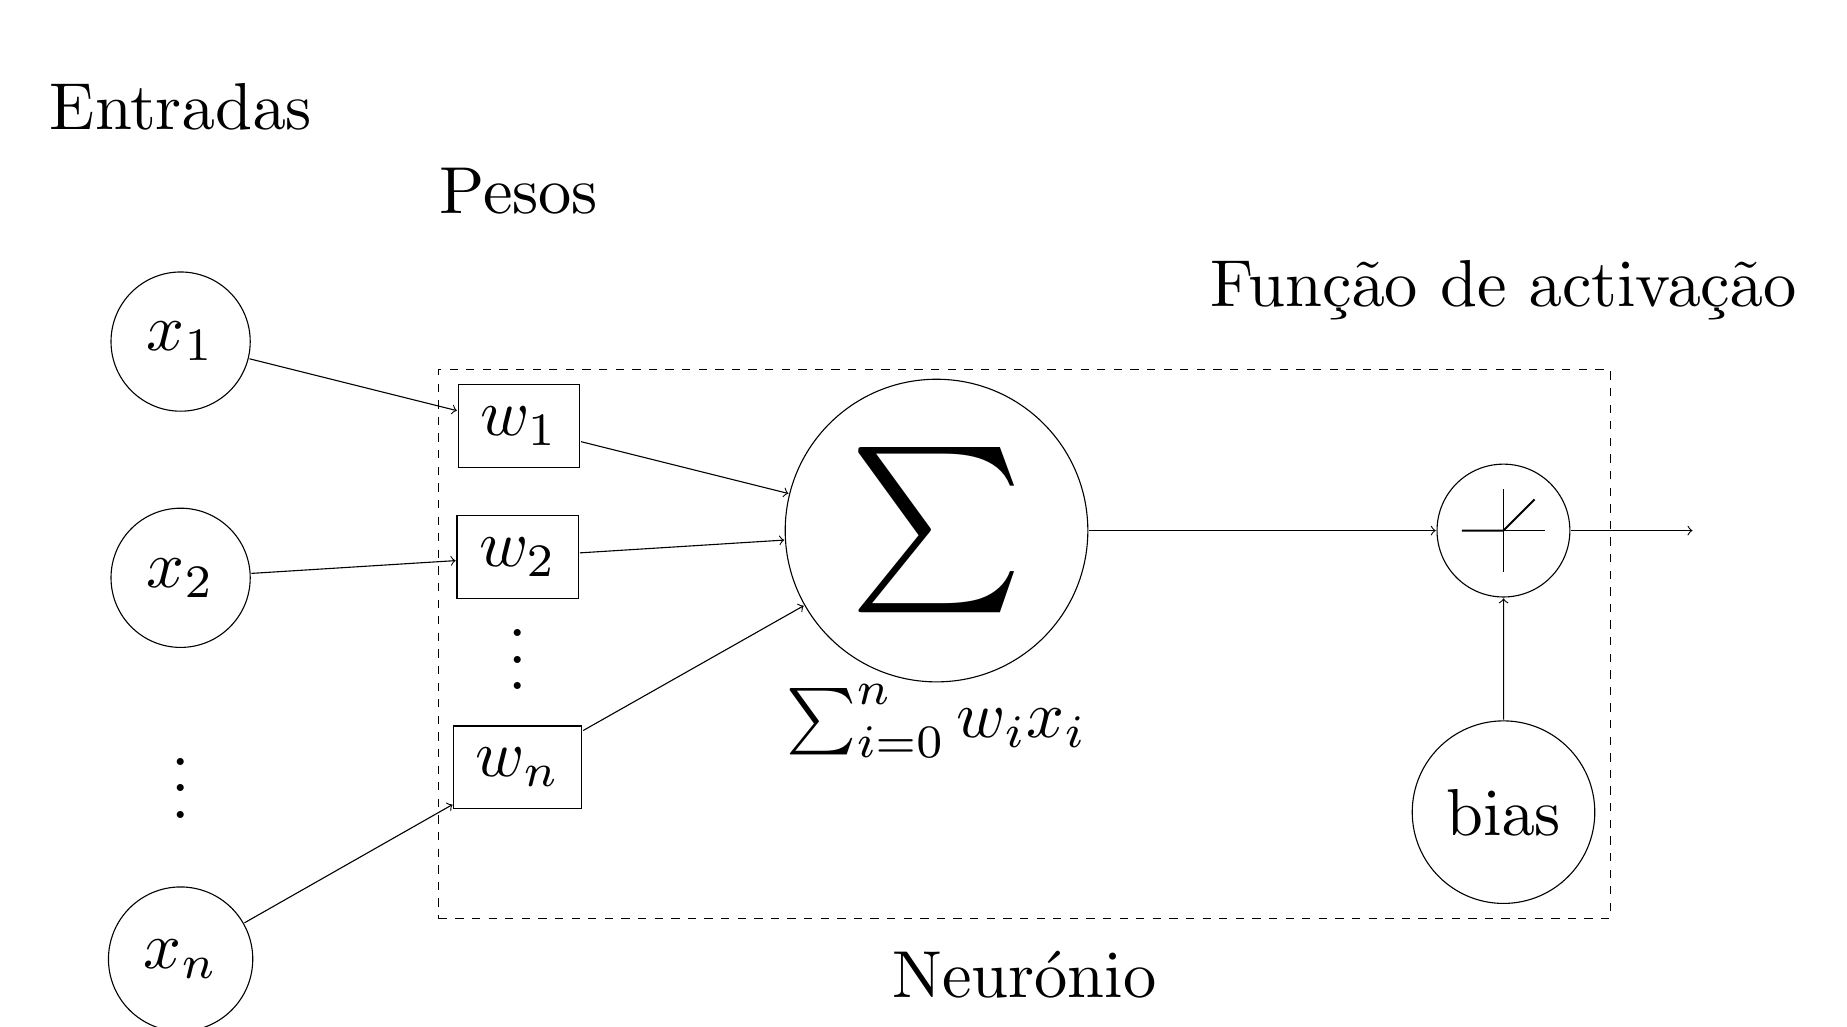
\begin{tikzpicture}[scale=2.4, transform shape]
    % Draw input nodes
    \foreach \h [count=\hi ] in {$x_2$,$x_1$}{%
          \node[input] (f\hi) at (0,\hi*1.25cm-1.5 cm) {\h};
        }
    % Dot dot dot ... x_n
    \node[below=0.62cm] (idots) at (f1) {\vdots};
    \node[input, below=0.62cm] (last_input) at (idots) {$x_n$};
    % Draw summation node
    \node[functions] (sum) at (4,0) {\Huge$\sum$};
    \node[below=0.69cm] at (sum) {$\sum_{i=0}^n w_ix_i$};
    % Draw edges from input nodes to summation node
    \foreach \h [count=\hi ] in {$w_2$,$w_1$}{%
          \path (f\hi) -- node[weights] (w\hi) {\h} (sum);
          \draw[->] (f\hi) -- (w\hi);
          \draw[->] (w\hi) -- (sum);
        }
    % Dot dot dot ... w_n
    \node[below=0.05cm] (wdots) at (w1) {\vdots};
    \node[weights, below=0.45cm] (last_weight) at (wdots) {$w_n$};
    % Add edges for last node and last weight etc
    \path[draw,->] (last_input) -- (last_weight);
    \path[draw,->] (last_weight) -- (sum);
    % Draw node for activation function
    \node[functions] (activation) at (7,0) {};
    \node[small_input, below=1cm] (bias) at (activation) {bias};
    \path[draw,->] (bias) -- (activation);

    % Place activation function in its node
    \begin{scope}[xshift=7cm,scale=1.25]
        \addaxes
        % flexible selection of activation function
        \relu
        % \stepfunc
    \end{scope}
    % Connect sum to relu
    \draw[->] (sum) -- (activation);
    \draw[->] (activation) -- ++(1,0);
    % Labels
    \node[above=1cm]  at (f2) {Entradas};
    \node[above=1cm] at (w2) {Pesos};
    \node[above=1cm] at (activation) {Função de activação};

    % Neuron
    \node[draw, dashed, fit= (w2) (last_weight) (activation) (bias), inner sep=0.5em] (square){};
    \node[below=1.5cm] at (square) {Neurónio};

\end{tikzpicture}}
% 	\caption{Ilustração de um neurónio. Adaptado de Haykin1999\cite{Haykin1999}}
% 	\label{fig:neuronio}
% \end{figure}


% A camada dense pega num input, cria um número de neurónios, \textit{N}, também chamado número de filtros, onde cada neurónio (filtro), recebe informação de cada uma das entradas, e todos os neuronios ligam a todas as dimensões de saida. \\
% Cada neurónio gera uma operação, inicialmente aleatória, para tentar reproduzir uma função que traduza a entrada na saída ideal. \\
% Esta camada é altamente influenciada pelo \textit{Perceptão} inicialmente proposto por Franck Rosenblatt\cite{Rosenblatt1958}. Este apresentava um \textit{Perceptão} que fazia uma decisão binária baseado na somas pesadas de todas as entradas. \\
% A ideia é a base utilizada actualmente, mas apresentava algumas limitações, e muita computação, o proposto por Minsky and Papert\cite{Minsky1969}, eleva a ideia com a introdução da funcção de activação e o bias. \\
% A utilização mais recorrente actual é a proposta por Haykin\cite{Haykin1999}, que baseada nas anteriores tem a seguinte apresentação:


% O conjunto destes neuroneis perfaz a camada de dense:

% \begin{figure}[H]
% 	\centering
% 	\resizebox{\linewidth}{!}{    \begin{tikzpicture}[scale=1.2]
    % Draw input nodes
    \foreach \h [count=\hi ] in {$x_2$,$x_1$}{%
          \node[input] (f\hi) at (0,\hi*1.25cm-1.5 cm) {\h};
        }
    % Dot dot dot ... x_n
    \node[below=0.62cm] (idots) at (f1) {\vdots};
    \node[input, below=0.62cm] (last_input) at (idots) {$x_n$};


    % Draw neurons nodes
    \foreach \h [count=\hi ] in {$N_2$,$N_1$}{%
          \path (f\hi) -- node[neurons] (w\hi) {\h} (sum);

          \draw[->] (f\hi) -- (w\hi);
        }
    % Dot dot dot ... w_n
    \node[below=0.05cm] (wdots) at (w1) {\vdots};
    \node[neurons, below=0.45cm] (last_neuron) at (wdots) {$N_n$};


    % Draw output nodes
    \foreach \h [count=\hi ] in {$y_2$,$y_1$}{%
          \path (w\hi) -- node[input] (o\hi) {\h} (sum);
        }
    % Dot dot dot ... w_n
    \node[below=0.05cm] (odots) at (o1) {\vdots};
    \node[input, below=0.45cm] (last_output) at (odots) {$y_n$};




    % Connect input nodes to hidden nodes
    \foreach \i in {1,2}{
        \foreach \j in {1,2}{
            \draw [->] (f\i) -- (w\j);
            \draw [->] (last_input) -- (w\j);
            }
        \draw [->] (f\i) -- (last_neuron);}
    \draw [->] (last_input) -- (last_neuron);

    % Connect hidden nodes to output nodes
    \foreach \i in {1,2}{    
        \foreach \j in {1,2}{
            \draw [->] (w\i) -- (o\j);
            \draw [->] (last_neuron) -- (o\j);
            }
        \draw [->] (w\i) -- (last_output);}
    \draw [->] (last_neuron) -- (last_output);
            


    % Labels
    \node[above=1cm]  at (f2) {inputs};
    \node[above=1cm] at (w2) {Neuronios};
    \node[above=1cm] at (o2) {Saidas};

    \end{tikzpicture}}
% 	\caption{Ilustração de uma camada dense.}
% 	\label{fig:dense}
% \end{figure}



% \subsection{Convolution\label{se:conv_layer}}

% A camada de convoluções difere da dense no sentido em que os filtros (neurónios) não são criados aleatoriamente, mas sim cada filtro trata de uma parte da camada de entrada.
% Nas convoluções é criada uma janela móvel que percorre a camada, criando um saida desse conjunto de pontos. Esta janela move-se sempre subsequentemente.\\
% Esta operação é normalmente feita na dimensão (ou dimensões) em que queremos perceber padrões. Nos nossos dados a convolução será na dimensão temporal. \\
% Se tivermos uma matriz com nove passos temporais (N,9,1), se o tamanho da janela de convulução for 3, teremos uma saida de tamanho 6 (N, 6, 1).

% \begin{figure}[H]
% 	\centering
% 	\resizebox{\linewidth}{!}{
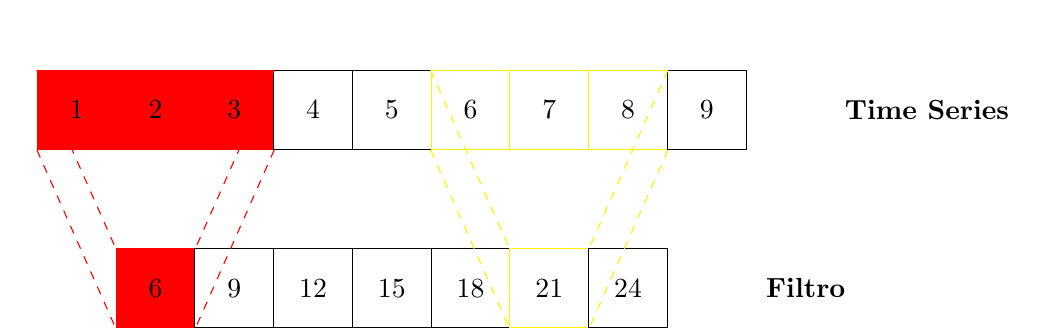
\begin{tikzpicture}
    % Time series
    \matrix (M1) [matrix of math nodes, nodes={draw, minimum size=1cm, anchor=center}, 
    column sep=-\pgflinewidth, row sep=-\pgflinewidth,
    ] {
        \node[fill=red, draw=red] (M1-1-1) {1}; & \node[fill=red, draw=red] (M1-2-1) {2};
        & \node[fill=red, draw=red] (M1-3-1) {3}; &
        4 & 5 & \node[draw=yellow] (M1-6-1) {6}; & \node[draw=yellow] (M1-7-1) {7};
        & \node[draw=yellow] (M1-8-1) {8}; & 9 \\
    };
    
    % Kernel
    \matrix (M2) [below=of M1, matrix of math nodes, nodes={draw, minimum size=1cm, anchor=center}, 
    column sep=-\pgflinewidth, row sep=-\pgflinewidth,
    ] {
        \node[fill=red, draw=red] (M2-1-1) {6}; & 9 & 12 & 15 & 18 & \node[draw=yellow] (M2-5-1) {21}; & 24 \\
    };

    \draw[dashed, red] (M1-1-1.north west) -- (M2-1-1.north west);
    \draw[dashed, red] (M1-3-1.north east) -- (M2-1-1.north east);
    \draw[dashed, red] (M1-1-1.south west) -- (M2-1-1.south west);
    \draw[dashed, red] (M1-3-1.south east) -- (M2-1-1.south east);

    \draw[dashed, yellow] (M1-6-1.north west) -- (M2-5-1.north west);
    \draw[dashed, yellow] (M1-8-1.north east) -- (M2-5-1.north east);
    \draw[dashed, yellow] (M1-6-1.south west) -- (M2-5-1.south west);
    \draw[dashed, yellow] (M1-8-1.south east) -- (M2-5-1.south east);

    
    % Titles
    \node [right=1cm, align=center, font=\bfseries] at (M1.east) {Time Series};
    \node [right=1cm, align=center, font=\bfseries] at (M2.east) {Filtro};
    \end{tikzpicture}}
% 	\caption{Ilustração da operação de Convolução}
% 	\label{fig:conv_layer1D}
% \end{figure}

% Anteriomente ignoramos o número de filtros. Mas as convuluções criam o número pedido de filtros para cada janela temporal. Aqui cada filtro vai funcionar como na camada dense, onde cada um começa com uma operação pseudo aleatoria. Esta operação está normalmente é feita na dimensão dos atributos. Ou seja, a quantidade de filtros que esta camada irá produzir por convulução. \\
% Se tivermos a mesma entrada que anterioemente mas com 4 atributos (N, 9, 4), e se definir o número de filtros para 2 teremos uma saida (N, 6, 2). \\
% Ou seja dois filtros por cada janela temporal. 


% \begin{figure}[H]
% 	\centering
% 	\resizebox{\linewidth}{!}{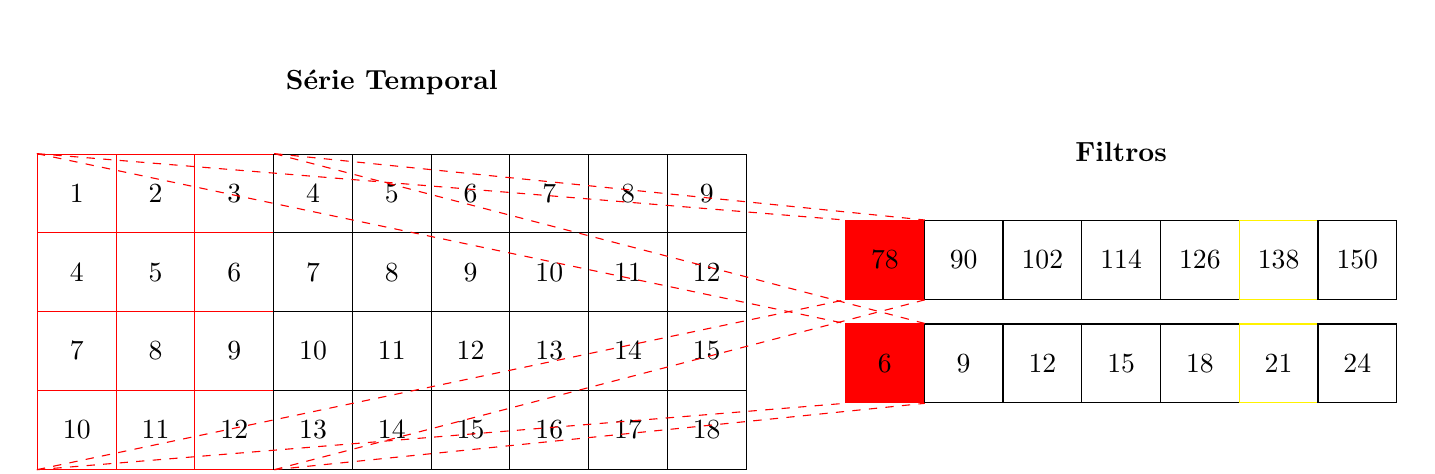
\begin{tikzpicture}[scale=2]
    \matrix (M1) [matrix of math nodes, nodes={draw, minimum size=1cm, anchor=center}, 
    column sep=-\pgflinewidth, row sep=-\pgflinewidth,]
{
    \node[draw=red] (M1-1-1) {1}; & \node[draw=red] (M1-1-2) {2}; & \node[draw=red] (M1-1-3) {3}; & 4 & 5 & 6 & 7 & 8 & 9\\
    \node[draw=red] (M1-2-1) {4}; & \node[draw=red] (M1-2-2) {5}; & \node[draw=red] (M1-2-3) {6}; & 7 & 8 & 9 & 10 & 11 & 12\\
    \node[draw=red] (M1-3-1) {7}; & \node[draw=red] (M1-3-2) {8}; & \node[draw=red] (M1-3-3) {9}; & 10 & 11 & 12 & 13 & 14 & 15\\
\node[draw=red] (M1-4-1) {10}; & \node[draw=red] (M1-4-2) {11};
& \node[draw=red] (M1-4-3) {12}; & 13 & 14 & 15 & 16 & 17 & 18\\
};

\matrix (M2) [matrix of math nodes, nodes={draw, minimum size=1cm, anchor=center}, 
column sep=-\pgflinewidth, row sep=0.3cm,
    right=of M1]
{
    \node[fill=red, draw=red] (M2-1-1) {78}; & 90 & 102 & 114 & 126 & \node[draw=yellow] (M2-1-5) {138}; & 150 \\
    \node[fill=red, draw=red] (M2-2-1) {6}; & 9 & 12 & 15 & 18 & \node[draw=yellow] (M2-2-5) {21}; & 24 \\
    };

% Titles
\node [above=0.5cm, align=center, font=\bfseries] at (M1.north) {Série Temporal};
\node [above=0.5cm, align=center, font=\bfseries] at (M2.north) {Filtros};
 
\draw[dashed, red] (M1-1-1.north west) -- (M2-1-1.north west);
\draw[dashed, red] (M1-1-1.north west) -- (M2-2-1.north west);

\draw[dashed, red] (M1-1-3.north east) -- (M2-1-1.north east);
\draw[dashed, red] (M1-1-3.north east) -- (M2-2-1.north east);

\draw[dashed, red] (M1-4-1.south west) -- (M2-1-1.south west);
\draw[dashed, red] (M1-4-1.south west) -- (M2-2-1.south west);


\draw[dashed, red] (M1-4-3.south east) -- (M2-1-1.south east);
\draw[dashed, red] (M1-4-3.south east) -- (M2-2-1.south east);



% TODO: add legenda em pequeno
%\node [right=1cm, align=center, font=\bfseries] at (matrix1.west) {Atributos};
%\node [right=1cm, align=center, font=\bfseries] at (matrix1.south) {tempo};


\end{tikzpicture}}
% 	\caption{Ilustração da camada de Convolução}
% 	\label{fig:conv_layer}
% \end{figure}

% As convuluções podem realizar as operaçoes em mais dimensões, é comun usar 2D para imegens, e 3D para videos. Nete trabalho apenas trabelhemos com convulucões 1D.\\


% \subsection{MaxPooling\label{se:max_pooling}}

% As camadas de pooling fazem operaçoes para redimensionar os filtros anteriores. \\
% Usando também uma janela movel, estas camadas esccolhem um dos valores da janelas para o resultado na saida. Operaações comuns de pooling são, o maximo, ou a media desses valores. Sendo que a operação é feita na dimensáo, ou nas dimensões, não dos filtros. \\
% Ou seja, se tivermos um tensor de formato (N, 4, 4), e tivermos uma janela de tamanho 3, iremos produzir uma reposta com o formato (N, 2, 4).\\
% Estas camadas são usadas principalmente para permitir uma escolha dos filtros mais relevantes e assim combater tanto overfitting como acelarar o processo de treino. \cite{Matoba2022}
% A camada usada nestas arquitecturas é MaxPooling, que escolhe o maior valor dentro da janela de strides, e aplica na saida. \\

% \begin{figure}[H]
% 	\centering
% 	\resizebox{\linewidth}{!}{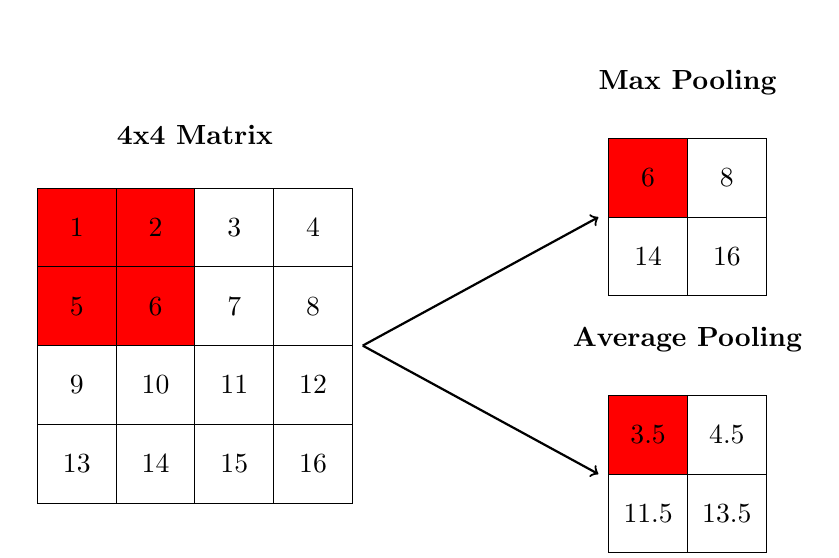
\begin{tikzpicture}
    % Max pooling 2x4 matrix (M2) on the right
    \matrix (M2) [matrix of math nodes, nodes={draw, minimum size=1cm, anchor=center}, 
    column sep=-\pgflinewidth, row sep=-\pgflinewidth,
    ] {
        \node[fill=red] (M2-1-1) {6}; & 8  \\
        14 & 16  \\
    };
    
    % Average pooling 2x4 matrix (M3) below M2
    \matrix (M3) [below=of M2, matrix of math nodes, nodes={draw, minimum size=1cm, anchor=center}, 
    column sep=-\pgflinewidth, row sep=-\pgflinewidth,
    ] {
        \node[fill=red] (M3-1-1) {3.5}; & 4.5 \\
        11.5 & 13.5 \\
    };
    
    % Node A halfway between M2 and M3
    \node (A) at ($(M2.south)!0.5!(M3.north)$) {};
    
    % 4x4 matrix (M1) on the left of node A
    \matrix (M1) [left=of A, xshift=-3cm,matrix of math nodes, nodes={draw, minimum size=1cm, anchor=center}, 
    column sep=-\pgflinewidth, row sep=-\pgflinewidth,
    ] {
        \node[fill=red] (M1-1-1) {1}; & \node[fill=red] (M1-1-2) {2}; & 3 & 4 \\
        \node[fill=red] (M1-2-1) {5}; & \node[fill=red] (M1-2-2) {6}; & 7 & 8 \\
        9 & 10 & 11 & 12 \\
        13 & 14 & 15 & 16 \\
    };
    
    % Draw arrows from M1 to M2 and M3
    \draw[->, thick] (M1.east) -- (M2.west);
    \draw[->, thick] (M1.east) -- (M3.west);
    
    % Titles
    \node [above=0.3cm, align=center, font=\bfseries] at (M1.north) {4x4 Matrix};
    \node [above=0.3cm, align=center, font=\bfseries] at (M2.north) {Max Pooling};
    \node [above=0.3cm, align=center, font=\bfseries] at (M3.north) {Average Pooling};
    \end{tikzpicture}}
% 	\caption{Ilustrção do efeito da camada de Pooling}
% 	\label{fig:pooling}
% \end{figure}



% \subsection{\href{https://keras.io/api/layers/regularization_layers/dropout/}{Dropout}\label{se:dropout}}

% Dropout é uma camada que elimina/ignora alguns dos neuronios da camada anterior. Este procedimente impede o overfitting, ajudando na generalização. \\

% \begin{figure}[H]
% 	\centering
% 	\resizebox{\linewidth}{!}{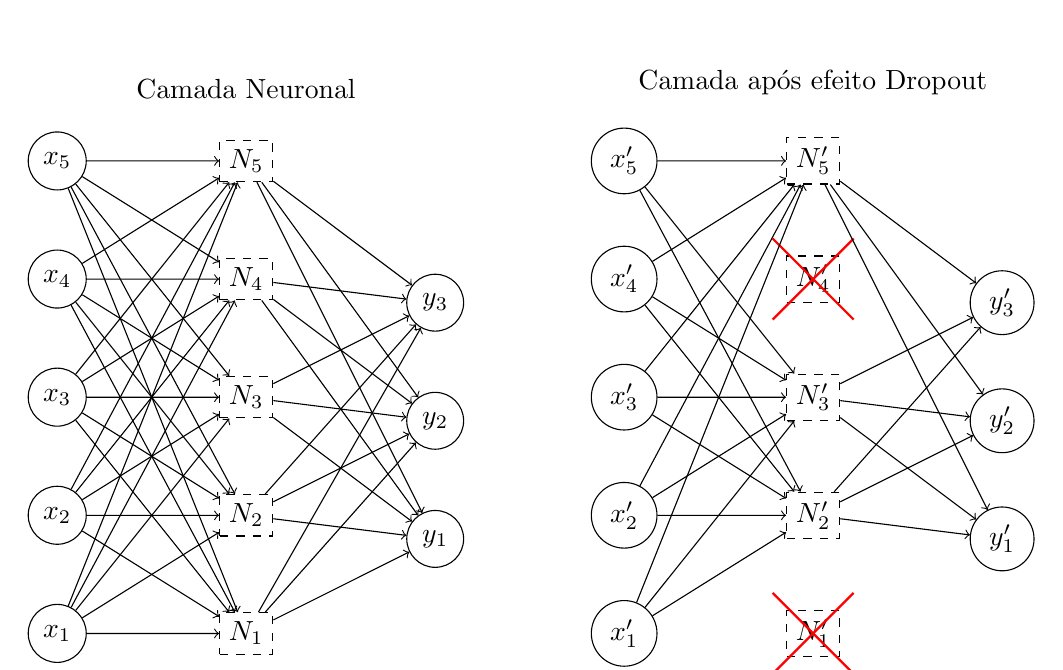
\begin{tikzpicture}[scale=1.2]
    % Group A
    \begin{scope}[local bounding box=groupA]
        % Draw input nodes
        \foreach \h [count=\hi ] in {$x_5$,$x_4$,$x_3$,$x_2$,$x_1$}{%
              \node[input] (f\hi) at (0,-\hi*1.25cm+1.5cm) {\h};
            }
    
        % Draw neurons nodes
        \foreach \h [count=\hi ] in {$N_5$,$N_4$,$N_3$,$N_2$,$N_1$}{%
              \node[neurons] (w\hi) at (2,-\hi*1.25cm+1.5cm) {\h};
            }

        \begin{scope}[yshift=-1.5cm, local bounding box=outs1]
            % Draw output nodes
            \foreach \h [count=\hi ] in {$y_3$,$y_2$,$y_1$}{%
                \node[input] (o\hi) at (4,-\hi*1.25cm+1.5cm) {\h};
                }
            \end{scope}

        % Connect input nodes to hidden nodes
        \foreach \i in {1,2,3,4,5}{
            \foreach \j in {1,2,3,4,5}{
                \draw [->] (f\i) -- (w\j);
                }
        }
    
        % Connect hidden nodes to output nodes
        \foreach \i in {1,2,3,4,5}{    
            \foreach \j in {1,2,3}{
                \draw [->] (w\i) -- (o\j);
                }
        }
    \end{scope}
    
    % Group B
    \begin{scope}[xshift=6cm, local bounding box=groupB]
        % Draw input nodes
        \foreach \h [count=\hi ] in {$x'_5$,$x'_4$,$x'_3$,$x'_2$,$x'_1$}{%
              \node[input] (f'\hi) at (0,-\hi*1.25cm+1.5cm) {\h};
            }
    
        % Draw neurons nodes
        \foreach \h [count=\hi ] in {$N'_5$,$N'_4$,$N'_3$,$N'_2$,$N'_1$}{%
              \node[neurons] (w'\hi) at (2,-\hi*1.25cm+1.5cm) {\h};
            }
    
        \begin{scope}[yshift=-1.5cm, local bounding box=outs]
            % Draw output nodes
            \foreach \h [count=\hi] in {$y'_3$,$y'_2$,$y'_1$}{%
                \node[input] (o'\hi) at (4,-\hi*1.25cm+1.5cm) {\h};
                }
            \end{scope}
        % Draw cross on the "deleted" neurons
        \foreach \i in {2,5}{
            \node[cross out, draw, red, thick, minimum size=1cm] (w'\i) at (2,-\i*1.25cm+1.5cm) {};
        }
    
        % Connect input nodes to hidden nodes
        \foreach \i in {1,2,3,4,5}{
            \foreach \j in {1,3,4}{
                \draw [->] (f'\i) -- (w'\j);
                }
        }
    
        % Connect hidden nodes to output nodes
        \foreach \i in {1,3,4}{    
            \foreach \j in {1,2,3}{
                \draw [->] (w'\i) -- (o'\j);
                }
        }
    \end{scope}
    
    % Add titles to each group
    \node[above=0.3cm] at (groupA.north) {Camada Neuronal};
    \node[above=0.3cm] at (groupB.north) {Camada após efeito Dropout};
    \end{tikzpicture}
    }
% 	\caption{Ilustrção do efeito da camada de dropout}
% 	\label{fig:dropout}
% \end{figure}



% \section{Blocos\label{se:blocos}}

% Todas as arquiteturas em análise irão ter por base um bloco de camadas neuronais. A formação dessas arquitecturas passa pelas diferentes maneiras que se pode utilizar o bloco principal. Repetições em serie ou em paralelo são um exemplo. \\

% \subsection{Bloco Dense\label{se:dense}}

% O bloco dense sendo ele o mais simples é formado por duas camadas Dense \ref{se:dense_layer} \cite{}, em que a primeira apresenta um número maior de filtros que a segunda. \\
% Estas camadas não são mais do que uma criação de filtros aleatórios combinando as entradas, para criar todos os filtros de saida. São a base das camadas intrepretativas. A acumulação em série (stacked) de camadas de dense está ligada a melhorias nas capacidades predictivas dos modelos \cite{VLHelen2021}. \\
% Exemplo ilustrativo do nosso bloco basico onde entrariam 16 filtros na primeira camada e para finalizar o bloco com 2 filtros \\




% \begin{figure}[H]
% 	\centering
% 	\resizebox{\linewidth}{!}{\begin{tikzpicture}[scale=1.2]
    % Draw input nodes
    \foreach \h [count=\hi ] in {$x_2$,$x_1$}{%
          \node[input] (f\hi) at (0,\hi*1.25cm-1.5 cm) {\h};
        }
    % Dot dot dot ... x_n
    \node[below=0.62cm] (idots) at (f1) {\vdots};
    \node[input, below=0.62cm] (last_input) at (idots) {$x_n$};


    % Draw neurons nodes
    \foreach \h [count=\hi ] in {$N1_2$,$N1_1$}{%
          \path (f\hi) -- node[neurons] (w\hi) {\h} (sum);

          \draw[->] (f\hi) -- (w\hi);
        }
    % Dot dot dot ... w_n
    \node[below=0.05cm] (wdots) at (w1) {\vdots};
    \node[neurons, below=0.45cm] (last_neuron) at (wdots) {$N1_n$};


    % Draw neurons nodes
    \foreach \h [count=\hi ] in {$N2_2$,$N2_1$}{%
          \path (w\hi) -- node[neurons] (ww\hi) {\h} (sum);

          \draw[->] (w\hi) -- (ww\hi);
        }
    % Dot dot dot ... w_n
    \node[below=0.05cm] (wwdots) at (ww1) {\vdots};
    \node[neurons, below=0.45cm] (last_neuronww) at (wwdots) {$N2_n$};



    % Draw output nodes
    \foreach \h [count=\hi ] in {$y_2$,$y_1$}{%
          \path (ww\hi) -- node[input] (o\hi) {\h} (sum);
        }
    % Dot dot dot ... w_n
    \node[below=0.05cm] (odots) at (o1) {\vdots};
    \node[input, below=0.45cm] (last_output) at (odots) {$y_n$};




    % Connect input nodes to hidden nodes
    \foreach \i in {1,2}{
        \foreach \j in {1,2}{
            \draw [->] (f\i) -- (w\j);
            \draw [->] (last_input) -- (w\j);
            }
        \draw [->] (f\i) -- (last_neuron);}
    \draw [->] (last_input) -- (last_neuron);


    % Connect hidden nodes to hidden nodes
    \foreach \i in {1,2}{    
        \foreach \j in {1,2}{
            \draw [->] (w\i) -- (ww\j);
            \draw [->] (last_neuron) -- (ww\j);
            }
        \draw [->] (w\i) -- (last_neuronww);}
    \draw [->] (last_neuron) -- (last_neuronww);

    % Connect hidden nodes to output nodes
    \foreach \i in {1,2}{    
        \foreach \j in {1,2}{
            \draw [->] (ww\i) -- (o\j);
            \draw [->] (last_neuronww) -- (o\j);
            }
        \draw [->] (ww\i) -- (last_output);}
    \draw [->] (last_neuronww) -- (last_output);
            


    % Labels
    \node[above=1cm]  at (f2) {inputs};
    \node[above=1cm] at (w2) {Neuronios};
    \node[above=1cm] at (ww2) {Neuronios};
    \node[above=1cm] at (o2) {Saidas};

    \end{tikzpicture}}
% 	\caption{Ilustrção do bloco de Dense}
% 	\label{fig:dense_block}
% \end{figure}




% \subsection{Bloco CNN\label{se:cnn}}

% Bloco de CNN é aqui definido como uma convolução na dimensão temporal seguido de camadas para combater o overfitting, MaxPooling e Dropout. \\


% %figura otima: https://www.researchgate.net/publication/344229502_A_Novel_Deep_Learning_Model_for_the_Detection_and_Identification_of_Rolling_Element-Bearing_Faults/figures?lo=1


% \begin{figure}[H]
% 	\centering
% 	\resizebox{\linewidth}{!}{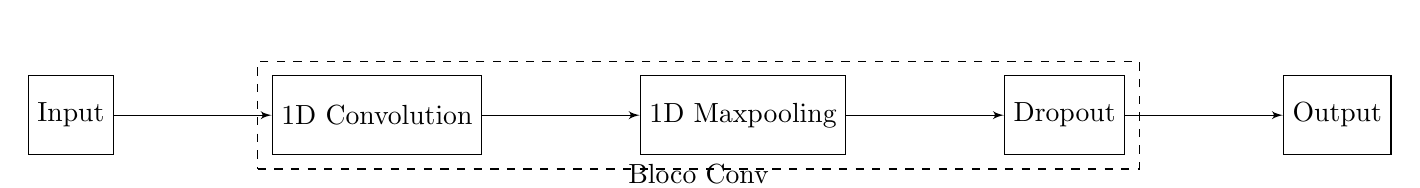
\begin{tikzpicture}[
    node distance = 2cm,
    auto,
    block/.style={
        rectangle,
        draw,
        align=center,
        minimum width=1cm,
        minimum height=1cm
    },
    line/.style={
        draw,
        -latex'
    }
]

    % Place nodes
    \node [block] (input) {Input};
    \node [block, right=of input] (conv) {1D Convolution};
    \node [block, right=of conv] (pool) {1D Maxpooling};
    \node [block, right=of pool] (dropout) {Dropout};
    \node [block, right=of dropout] (output) {Output};

    % Draw edges
    \path [line] (input) -- (conv);
    \path [line] (conv) -- (pool);
    \path [line] (pool) -- (dropout);
    \path [line] (dropout) -- (output);

    % Neuron
    \node[draw, dashed, fit= (conv) (pool) (dropout), inner sep=0.5em] (square){};
    \node[below=0.5cm] at (square) {Bloco Conv};

\end{tikzpicture}
}
% 	\caption{Ilustração do bloco de CNN}
% 	\label{fig:cnn_block}
% \end{figure}



% \subsection{Bloco LSTM\label{se:lstm}}

% O uso de LSTM para previsões é uma area comum, mas aqui é seguido através das ideas partilhas em \cite{Hewamalage2021}, e reforçado pelo uso em previsões energéticas demonstados em \cite{Costa2022} \\
% O bloco LSTM é a aplicação das RNN, aqui sendo apenas definido como uma camada de LSTM. \\
% Estes blocos mantêm dentro de si ligações a diferentes camadas temporais, e cada filtro criado, mantêm uma "memória" dos filtros passados. \\
% Bastante utilizado em modelação de linguagem.

% imagem


% \section{Arquiteturas \label{se:arquitecturas}}

% \subsection{Vanilla \label{se:vannila}}

% O termo "Vanilla" aqui é aplicado para aquitecturas que apenas usam um bloco de cada, um de entrada, um principal, e um interpretativo. \\
% Como exemplo a arquitetura de "VanillaCNN" utiliza o bloco de convulução apenas para terminar com uma camda interpretativa.


% \subsection{Stacked\label{se:stacked}}

% Stacked refere-se a "amontoado" onde se utiliza o bloco principal várias vezes em série.E apenas um bloco de  entrada e um interpretativo. \\
% Como exemplo a arquitetura de "StackedCNN" utiliza dois blocos (ou mais) de convulução depois da camada de entrada, e finaliza com uma camada interpretativa.

% imagem da mesma



% \subsection{UNET\label{se:UNET}}

% Normalmente usando em modelção de imagens, a arquitectura UNET passa por criar uma rede de expansão dos filtros, usando convoluções, e de seguida uma rede de contracção dos mesmo, até aos tamanhos pretendidos.\\
% O bloco principal contextualmente o mesmo que o CNN.\\
% Nas suas ligações UNET junta informação de filtros passados (não de nivel temporal mas de rede neuronal) para realçar informação já trabalhada, e assim identificar padrões de vários contextos diferentes.\\
% É habitual também adicionar aos blocos principais portões de atenção, portões residuais. Estas duas tecnicas são também estudadas aqui.\\
% É chamada assim pois é uma rede (NET) que forma um U na sua expansão e contracção.\\

% Como exemplo a arquitetura de "UNET"

% imagem da mesma


% \section{Considerações adicionais\label{se:modelos_plus}}

% Os modelos testados são combinações destes blocos e aquitecturas. 

\label{ch:arch}
% Ferramentas
\newpage
\thispagestyle{plain}
\chapter{Ferramentas}

\section{\href{https://github.com/alquimodelia/alquimodelia}{Alquimodelia}\label{se:alquimodelia}}


Com o propósito de desenvolver este estudo, e deixar ferramentas para a replicação do mesmo, foi criado uma biblioteca em python para desenhar as arquitecturas em estudo.\\

\subsection{Construtor de modelos}

Seguindo as arquitecturas descritas anteriormente esta ferramenta constrói os modelos automaticamente, sendo que precisamos apenas de fornecer os parâmetros variáveis. Permitindo assim um fácil teste de vários tipo de modelos, não tendo de reescrever código para cada um deles.\\

\subsection{\href{https://github.com/alquimodelia/alquitable/blob/main/alquitable/generator.py}{Gerador de dados}}

O gerador construido trata da formatação dos dados para entrada nos modelos. Formatação esse que se baseia nos valores de janelas temporais a usar, e na divisão treino/teste.\\
Esta ferramenta agrega os dados em tensores de formato \textit{(N, t, a)}, onde \textit{N} é o número de casos, \textit{t} é a janela temporal, e \textit{a} é o número de atributos.\\
A ferramenta permite também definir o tempo de salto entre cada entrada.\\
Usando como exemplo uma janela temporal de 168 (horas, uma semana) para treino, e 24 (horas) para o alvo. Com um salto temporal de 1 a primeira entrada teria como treino as primeiras 168 horas dos dados, e como alvo as 24 horas consequentes. A segunda entrada seria a partir da segunda hora dos dados, e assim consecutivamente. Para um caso em que o tempo de salto seria 24, a primeira entrada mantinha-se, mas a segunda começaria 24 horas depois, e não apenas uma.\\

Como estamos também a lidar com dados desfasados, o gerador atribui este desfasamento em atributos a especificar. No caso em estudo temos que os atributos são de DA (day-ahead), logo estão desfasados 24 horas. O que implica termos de aplicar este desfasamento nos dados que não são DA, nomeadamente os dados alvo. Esta propriedade permite também o fácil uso da ferramenta noutros dados desfasados, como as previsões a 3 ou 8 horas.\\

\section{\href{https://github.com/alquimodelia/MuadDib}{MuadDib}\label{se:muaddib}}

Esta ferramenta criada para desenvolver as experiências desta dissertação, permite ao utilizador apenas com os dados que quer utilizar e a especificação das métricas pretendidas, facilmente ter um modelo optimizado para os seus dados e problema.\\
Ao usar a ferramenta o utilizador consegue testar vários modelos e hiper parametrizações diferentes mas mantendo a necessidade de escrever código ao mínimo.\\
\label{ch:ferramentas}
\newpage
\thispagestyle{plain}
\chapter{Métricas}

As métricas utilizadas serviram maioritariamente dois propósitos, com valorizações distintas na escolha de melhores modelos.\par
O primeiro intuito é de estudo de cada modelo, utilizando as métricas comuns de regressão linear, comparando os valores reais com os valores das previsões.\par
Outro objectivo das métricas aplicadas e este mais relevante, era o estudo comparativo do desempenho de cada modelo com o modelo de benchmark.\par

\begin{alignat*}{3} 
& t : \text{Valor real.} &\qquad& p : \text{Previsão} &\qquad& n : \text{número de amostras} \\
\end{alignat*}


\section{Métricas de modelo}

\bigskip
RMSE - Root Mean Squared Error \\

\begin{equation} \label{eq:rmse} 
    RMSE = \sqrt{\frac{1}{n} \sum_{i=1}^{n}(t_i - p_i)^2} 
\end{equation}
\smallskip

Métrica comum em problemas de regressão, dando mais peso a erros maiores, mas retorna um valor que pode ser diretamente comparado ao valor em estudo. Neste caso podemos considerar que o RMSE representa o erro quadrático em MWh.\par
\bigskip
SAE - Sum Abs Error \\


\begin{equation} \label{eq:sae} 
    SAE = \sum_{i=1}^{n}\left|t_i - p_i \right|
\end{equation}
\smallskip

Este simboliza a soma absoluta de todos os erros, dentro da janela temporal em questão. Que representa a quantidade total da energia alocada/não alocada em erro, este é também a soma das duas próximas métricas.\par
\bigskip
AllocF - Alocação em Falta \\

\begin{equation} \label{eq:allocf} 
    AllocF = 
    \begin{cases} 
        0 & , \text{se } p \geq t \\
        t - p  & , \text{se } p < t \\
    \end{cases} 
\end{equation}
\smallskip

Representa a soma total de toda a energia que faltou ser alocada.\par
\bigskip
AllocD - Alocação em Demasia \\

\begin{equation} \label{eq:allocd} 
    AllocD = 
    \begin{cases} 
        0 & , \text{se } p \leq t \\
        p - t  & , \text{se } p > t \\
    \end{cases} 
\end{equation}
\smallskip

Representa a soma total de toda a energia que for alocada em demasia.\par

\section{Métricas de comparação modelo/benchmark}

GPD - Ganho Percentual de Desempenho

\begin{equation} \label{eq:gpd} 
    GPD = \frac{SAE_{benchmark} - SAE_{modelo}}{SAE_{benchmark}} \times 100
\end{equation}
\smallskip

O Ganho Percentual de Desempenho é a nossa métrica basilar. Representa, dentro da janela temporal de validação, a percentagem de melhoria do modelo em relação ao benchmark. Isto é representa a percentagem de energia que foi melhor alocada que o modelo. Onde 100\% representa uma melhoria perfeita, onde o modelo não tem erro. E 0\% representa nenhuma melhoria, ou seja, igual ao benchmark. Pode também ter valores negativos, que representa a percentagem em que o modelo é pior que o benchmark, podendo ser infinitamente pior.\par
Esta métrica é representativa da totalidade de energia, tanto alocado como em falta.\par
As próximas métricas são variações desta que ajudam a escolher o melhor modelo em cada experiência, conseguindo distinguir entre alocação em falta e em demasia.\par
\bigskip
GPDF - Ganho Percentual de Desempenho (alocação em) Falta\\

\begin{equation} \label{eq:gpdf} 
    GPDF = \frac{AllocF_{benchmark} - AllocF_{modelo}}{AllocF_{benchmark}} \times 100
\end{equation}
\smallskip

O mesmo que o GPD mas apenas para as somas totais de alocação em falta.\par
\bigskip
GPDD - Ganho Percentual de Desempenho (alocação em) Demasia\\

\begin{equation} \label{eq:gpdd} 
    GPDD = \frac{AllocD_{benchmark} - AllocD_{modelo}}{AllocD_{benchmark}} \times 100
\end{equation}
\smallskip

O mesmo que o GPD mas apenas para as somas totais de alocação em falta.\par
\bigskip
GPD Norm - Ganho Percentual de Desempenho Normalizado \\

\begin{equation} \label{eq:gpdnorm} 
    GPD Norm = \frac{GPDF + GPDD}{2}
\end{equation}
\smallskip

Aqui o GPD é calculado a partir dos já calculados GPDF e GPDD, sendo a média destes. Desta maneira conseguimos ter uma percentagem de melhoria em relação ao benchmark, onde a melhoria da alocação em demasia e a melhoria da alocação em falta têm o mesmo peso.\par

\bigskip
GPD $Norm^{2}$ - Ganho Percentual de Desempenho Normalizado (negativos) Quadrado

 GPD $Norm^{2}$=GPD norm mas os GPD são ao quadrado se forem negativos  


 \begin{equation} \label{eq:gpdnorm2} 
    GPD Norm^{2} = 
    \begin{cases} 
        GPD Norm & , \text{se } GPDF \text{ }\&\text{ } GPDD \geq 0 \\
        \frac{GPDF^{2} + GPDD}{2} & , \text{se } GPDF  < 0 \\
        \frac{GPDF + GPDD^{2}}{2} & , \text{se } GPDD < 0 \\
    \end{cases} 
\end{equation}
\smallskip


O mesmo que GPD norm mas os GPDF ou GPFD que sejam negativos o seu valor é ao quadrado e mantendo-se negativo. Serve para dar mais peso aos valores negativos, assim não tendo GPD altos mesmo se um dos GPD for negativo (pior que o benchmark).\par
Esta métrica é a principal na escolha do melhor modelo em cada experiência visto manter ambos os GPD mas penalizando se algum deles é negativo.\par
\bigskip
GPD Positivo  - Ganho Percentual de Desempenho Positivo

 \begin{equation} \label{eq:gpdpositivo} 
    GPD Positivo = 
    \begin{cases} 
        GPD & , \text{se } GPDF \text{ }\&\text{ } GPDD \geq 0 \\
        0 & , \text{se } GPDF \text{ }\|\text{ } GPDD < 0 \\
    \end{cases} 
\end{equation}
\smallskip


Esta métrica é igual a GPD mas apenas nos casos em que ambos são positivos, logo o modelo é melhor que o benchmark, senão é zero. Serve para medir o GPD real, mas apenas nos casos em que o modelo já surpassa o benchmark.\par
\label{ch:metricas}

% Métodos
\newpage
\thispagestyle{plain}
\chapter{Métodos}

A todas as experiências foram aplicadas as métricas apresentadas, excepto no benchmark onde teríamos métricas de comparação a ele próprio.\\
Para a escolha de melhor modelo dentro das experiências foi escolhido o modelo que melhor resultados apresentou para a métrica em questão. Sendo esta o GPD $Norm^{2}$ enquanto não encontramos uma melhoria tanto na alocação em falta como na em demasia, ao que se seguida foi usado o GPD Positivo.\\
No caso das Redes Neuronais a hiper parametrização foi feita também deste modo, sendo que primeiro se encontrou uma hiper parametrização adequada aos dados, usando uma arquitetura simples e só depois com essa configuração foi feita a experiência  nas várias arquiteturas.\\
O objectivo é conseguir um modelo que tenha a uma Alocação Total em Falta e Alocação Total em Demasia menor que o Benchmark, dentro dos anos 2019 a 2022. Logo em termos de métricas um GPD Positivo mais elevado possível.\\

\thispagestyle{plain}
\section{Estatisticos}

Em estatística conseguimos encontrar vários métodos de estudo de séries temporais. Estes métodos são normalmente usados como primeira abordagem para fazer previsões.\par
Estes modelos podem ser \gls{AR}, onde vão fazer previsões baseados num número \textit{(p)} de dados anteriores. Estes modelos são construídos com a noção de que um valor é linearmente dependente de \textit{p} valores anteriores numa série temporal.\par

\begin{alignat*}{2} 
    & X_{t} : \text{Valor no } t \text{ a prever.} &\quad& p : \text{O número observaçoes anteriores.} \\
    & \varphi_{i} : \text{Coeficiente na observação } i. &\quad& q : \text{O número observaçoes anteriores.} \\
    & \epsilon_{i} : \text{Erro na observação } i. &\quad& \theta_{i} : \text{Coeficiente na observação } i \text{.} \\ 
    & \mu : \text{Média dos valores } X \text{.} 
\end{alignat*}

\bigskip
\gls{AR} \\

\begin{equation} \label{eq:ar} 
    X_{t} = \sum_{i=1}^{p}\varphi_{i} X_{t-i} 
\end{equation}
\smallskip

Outra família destes modelos são os de \gls{MA}, onde a média de um número de observações \textit{(q)} em conjunto com os erros \textit{($\epsilon$)} e os coeficientes \textit{($\theta$)} é usada para prever os valores seguintes.\par
\bigskip
\gls{MA} \\

\begin{equation} \label{eq:ma} 
    X_{t} = \mu + \sum_{i=1}^{q}(\theta_{i} \epsilon_{t-i}) + \epsilon_{t}
\end{equation}
\smallskip
Estes dois tipos de modelos podem ser juntos criando os modelos \gls{ARMA}. que junta as capacidades dos modelos anteriores.\par

\bigskip
\gls{ARMA} \\

\begin{equation} \label{eq:arma} 
    X_{t} = \sum_{i=1}^{p}\varphi_{i} X_{t-i}  + \mu + \sum_{i=1}^{q}(\theta_{i} \epsilon_{t-i}) + \epsilon_{t}
\end{equation}
\smallskip

Existem mais modelos de previsão estatística baseados nestes com algumas variações, mas para este trabalho, e apenas como ponto de comparação às redes neuronais, ficamos apenas por estes.\par
As variáveis em estudo por tipo de modelo foram retiradas das autocorrelações temporais usando os métodos de sugestão da ferramenta \hyperref[se:muaddib]{MuadDib}:\\


\begin{table}[h] \centering
\begin{tabular}{lrrrr}
    \toprule
     & p & q \\
    \midrule
    \gls{AR} & 1/ 2 / 23 / 24 / 25 / 48 / 144 / 168 / 192 / 336 & NA \\
    \gls{MA} & NA & 1 / 24 \\
    \gls{ARMA} & 1 & 1 \\
    \bottomrule
    \end{tabular}
    \label{tab:varsstats} 
    \caption{Variáveis de estudo dos modelos AR/MA}
\end{table}


Todos estes modelos foram testados usando o software disponível na package de python \href{https://www.statsmodels.org/stable/index.html}{statsmodel}, com a classe \href{https://www.statsmodels.org/stable/generated/statsmodels.tsa.arima.model.ARIMA.html}{ARIMA}.
 \label{se:metstats}


\newpage
\thispagestyle{plain}
\section{Redes Neuronais}

As redes neuronais podem ser descritas como uma função desconhecida \textit{f(x)=y} onde durante o treino a função \textit{f} é criada através da manipulação dos pesos da sua arquitetura usando os dados de treino, x, de forma a diminuir ao máximo uma função de perda . Sendo \textit{f'(x)=y'} um modelo já treinado onde \textit{y'} é a previsão, a função de perda \textit{fp(y, y')} idealmente igual a 0, com \textit{y'=y.}\\
Neste trabalho o \textit{x} são todos os dados apresentados no capitulo \hyperref[ch:estudo_2]{Estudo 2}, em grupos de 128 (horas), e o \textit{y} é a energia usada, "UpwardUsedSecondaryReserveEnergy" no modelo de previsão de energia a subir e "DownwardUsedSecondaryReserveEnergy" no modelo de previsão de energia a descer, nas 24 horas subsequentes. A \textit{fp} é um dos factores de estudo, assim como outros parâmetros dentro das arquiteturas de modelos, \textit{f}.\\
Assim utilizamos os 168 horas (1 semana) para prever as 24 horas seguintes. As 24 horas seguintes são o objectivo do estudo, energia a alocar no dia seguinte. As 168 horas são escolhidas graças às \hyperref[tab:tempcorr]{maiores autocorrelações temporais}, de onde as maiores fora das primeiro 48 horas são 144, 168, 192 horas ou seja, 6, 7 e 8 dias respectivamente, onde em ambos os casos 7 dias era o valor com maior correlação.\\
As condições em estudo são feitas através da ferramenta \hyperref[se:muaddib]{MuadDib}, seguindo vários percursos entre as combinações possíveis, de modo a conseguir a combinação óptima, maior GPD Positivo.\\


\subsection{Arquitecturas}

\gls{FCNN}, \gls{CNN} , RNN são as arquitecturas mais simples que vamos estudar. Estas vão apenas pegar nos blocos e vamos criar as mesmas "Vanila" e "Stacked" com 2 blocos (ex: StackedCNN) ou 6 blocos (ex: Stacked6CNN).\\
UNET, \gls{LSTM} são arquiteturas mais complexas e pesadas. Como descrito anteriormente uma mais utilizada em análise de imagens, e outra em análise de texto respectivamente.\\
Transformers são as mais pesadas qualidade comum da família de "generative AI".

\subsection{Função de Perda}

Nos primeiros testes mais simples foi imediato a discrepância entre os erros da energia alocada em demasia e em falta. Sendo que estes erros estão em dimensões completamente diferentes.
\begin{figure}[H]
    \centering
    \includegraphics[width=\textwidth]{plots/allocs_results_shadow.png}
    \caption{Resultados de alocações totais em diferentes arquiteturas}
    \label{fig:resexparchs}
  \end{figure}

Na energia em falta, estamos a lidar com valores na dimensão de $10^{6}$ nos resultados, sendo que o benchmark está nos $10^{5}$. Logo estão bastante acima do que queremos. Por outro lado na Energia em Demasia temos resultados na ordem dos $10^{6}$ e o benchmark está na ordem dos $10^{7}$. Isto dá-nos espaço para aumentar os resultados da Energia em Demasia mantendo-os ainda abaixo do benchmark para diminuir os resultados da Energia em Falta com objectivo de a ter também abaixo do benchmark.\\
Para combater esta desigualdade foram criadas várias funções de perda para atribuir melhor peso a ambas de modo a atingir melhor o objectivo geral.\\
De maneira que partimos esta experiência em duas partes. A primeira parte, Função de Perda Avançada, vai estudar diferentes maneiras de distribuir pesos entre a energia alocada em demasia e a em falta. A segunda vai escolher qual a melhor função de perda a aplicar nessa distribuição de pesos, ou vice-versa.\\


\subsubsection{Funções de Perda}
Depois de escolhidos os pesos nos diferentes grupos são testadas as funções a aplicar. Aqui vamos manter simples e testar apenas as mais comuns em problemas de regressão linear: \gls{MAE}, \gls{MSE}, \gls{MSLE}.\\
\gls{MAE} é usada no geral em problemas em que os dados têm um histograma linear, e um erro normalmente distribuído.\\
\gls{MSE} é usado para atribuir maior peso aos erros maiores, do que no \gls{MAE}. Fazendo com que o modelo se concentre mais em aprender a diminuir erros maiores.\\
\gls{MSLE} é sugerido em dados que têm uma histograma exponencial.\\

% TODO: meter formulas? depende do espaço


\subsubsection{Função de Perda Avançada}\label{se:advancedloss}

Para escolher a melhor maneira de distribuir pesos foi criada uma função de perda com diferentes regras, que distribuem o peso da amostra.\\
\href{https://github.com/alquimodelia/alquitable/blob/main/alquitable/advanced_losses.py#L33}{Mirror Weights (Pesos Espelhados)}\\
Que vai distribuir os pesos da amostra consoante um rácio predefinido e o próprio erro da amostra.\\
Os pesos nas amostras vão ser divididos entre os erros negativos (alocação em demasia) e os positivos (alocação em falta). Consoante uma variável lógica,  uns terão peso 1 e os outros serão o próprio erro em absoluto. Dando assim um peso equivalente ao erro, quanto maior o erro maior o peso da amostra na função de perda, do lado da amostra escolhido (em demasia ou em falta).\\
Pode ser multiplicado um rácio tanto a um dos pesos como a outro, sendo estes rácios que irão equilibrar as diferenças entre a alocação em falta e a em demasia. E o sinal do rácio influencia qual o lado a ser multiplicado.\\
Este pesos são passados directamente à função de perda em uso.\\

% TODO: meter formulas? depende do espaço

\begin{figure}[H]
    \centering
    \includegraphics[width=\textwidth]{plots/ratio_mw.png}
    \caption{Resultados de alocações totais em diferentes rácios}
    \label{fig:resexpratiomw}
  \end{figure}

Estas variações no rácio produzem diferentes dimensões nas alocações, modificando assim a sua posição em relação ao benchmark. Aqui para cada arquitetura o rácio ideal para o melhor GPD Positivo diferencia ligeiramente, tendo sido procurado com tentativa/erro baseado em assunções perante a aparente distribuição rácio/alocações.\\


\subsection{Função de Activação}

Como mostrado em \cite{Vaswani2017}, e \cite{Liu2022} , o uso de uma activação mais apropriada aos dados pode ser crucial para um salto na qualidade do modelo.\\
Vamos dividir as função de activação usadas nas camadas intermédias e a usada na camada final. Isto porque as camadas intermédias tendem a funcionar melhor com a mesma activação e a final é que mais define o valor que sai do modelo.\\
Esta experiência vai testar a combinações das seguintes activações nas duas variáveis descritas anteriormente: linear, relu, gelu.\\


\subsection{Pesos}
Esta experiência serve para testar diferentes pesos por amostra, não por grupo como na experiência anterior. Aqui os pesos são aplicados no momento da função de perda final.\\
Normalmente é usado para dar mais pesos a amostras com menor amostragem. Mais facilmente aplicável em modelos de classificação. Com este é um problema de regressão linear com séries temporais vamos testar aplicar os seguintes pesos, ou nenhum peso.\\
Este peso é multiplicado peso peso em \hyperref[se:advancedloss]{peso espelhados}.


\subsubsection{Temporais}
Aqui a primeira amostra tem o menor valor de peso (1) e todas as amostras seguintes incrementam 1. Dando mais peso consecutivamente a amostras mais recentes. É testado em vários casos de séries temporais onde o objectivo é prever o futuro. Podendo assim dar mais peso a tendências e valores mais recentes.\\

\subsubsection{Distância à média}
Neste peso cada amostra tem como valor a sua distância à média total dos dados. Vai servir para o modelo conseguir criar pesos relevantes a valores mais distantes à média.\\
Logo as amostras que tenham picos de valores têm um peso maior, forçando o modelo a aprender melhor estas ocasiões.

 \label{se:metneuralnet}

\thispagestyle{plain}
\section{Dados de Validação}
Os dados de validação são os mesmos que os dados de treino, embora apenas durante os anos de 2019 a 2022, inclusive.\\
Usamos como benchmark as capacidades alocadas, "SecondaryReserveAllocationAUpward" e "SecondaryReserveAllocationADownward", e como validação e objectivo, \hyperref[se:metneuralnet]{y}, a própria energia usada, "UpwardUsedSecondaryReserveEnergy" e "DownwardUsedSecondaryReserveEnergy".

\section{Benchmark}

Como método de comparação a todas as experiências foi criado uma base que servirá de benchmark.\\
Este base não é nada mais do que a própria previsão feita pela entidade reguladora \gls{ESIOS}. Dentro do nossos dados são os valores nos campos "SecondaryReserveAllocationAUpward" e "SecondaryReserveAllocationADownward".\\
Para os dados utilizados, podemos ver a totalidade e comparação do benchmark (Energia Alocada) com a energia utilizada.\\

\begin{figure}[H]
    \centering
    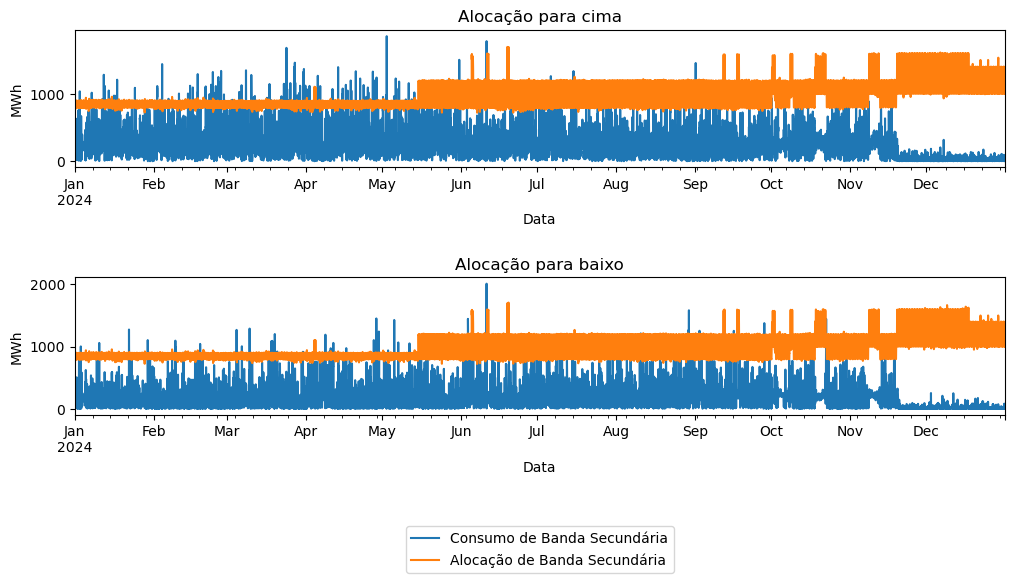
\includegraphics[width=\textwidth]{plots/benchmark_alocacoes_validacao.png}
    \caption{Série Temporal dos dados de Benchmark c/ consumo real}
    \label{fig:benchmarktimeseries}
\end{figure}

Imediatamente podemos verificar que o método para prever a energia necessária actualmente está dentro de um espectro limitado de valores, sendo que esses valores estão perto dos valores de ponta na alocação para cima, e perto dos valores médios na alocação para baixo.\\
Isto deve-se ao facto de ser uma função fixa, baseado no dia em questão. Notamos também que a meio de 2022 houve uma mudança dessa função que limitou os alcances tornando os valores mais elevados. Devido à guerra na Ucrânia e à forte incerteza que esta trouxe aos mercados de eletricidade por causa da crise de gás na Europa, que aumentou significativamente o preço deste recurso e levou à adaptação dos consumidores e países, a Red Eléctrica de España (\gls{REE}) aumentou as necessidades de reserva secundária para responder a esta incerteza.\\
Do ponto de visto de dados faz sentido para diminuir a quantidade  de vezes em que não é alocada energia suficiente.\\
Mas o mais importante a notar é a forma estática destes métodos, dado a natureza flutuante dos da energia necessária este método apresenta frequentemente um erro grande.\\
Podemos ver em pormenor analisando algumas janelas temporais dentro do período de validação. Vendo o melhor e pior resultado, em termos de erro absoluto, em janelas temporais de ano, mês, semana e dia.\\


\begin{figure}[H]
    \centering
    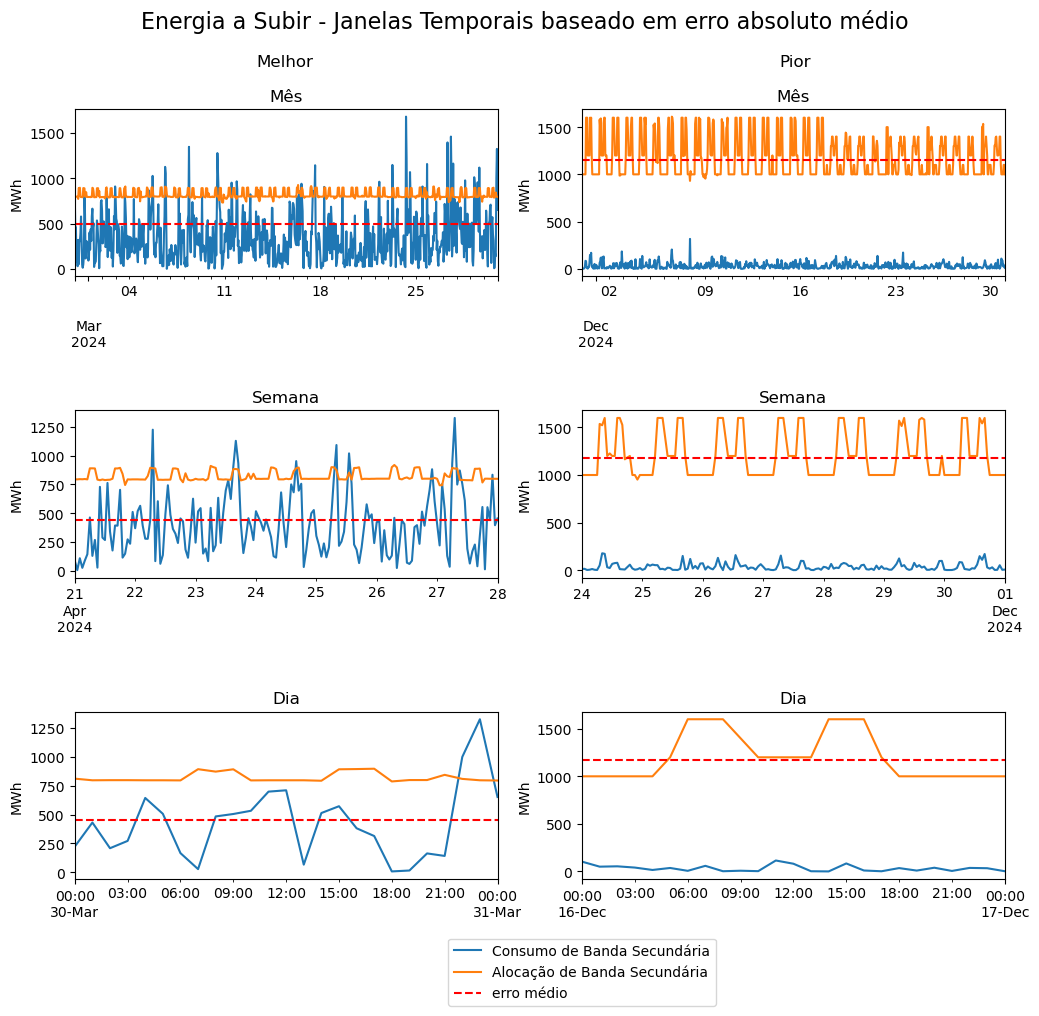
\includegraphics[width=\textwidth]{plots/alocacoes_temporais_upward_dataset.png}
    \caption{Janelas temporais de benchmark energia a subir}
    \label{fig:benchmarktimewindowsup}
\end{figure}


\begin{figure}[H]
    \centering
    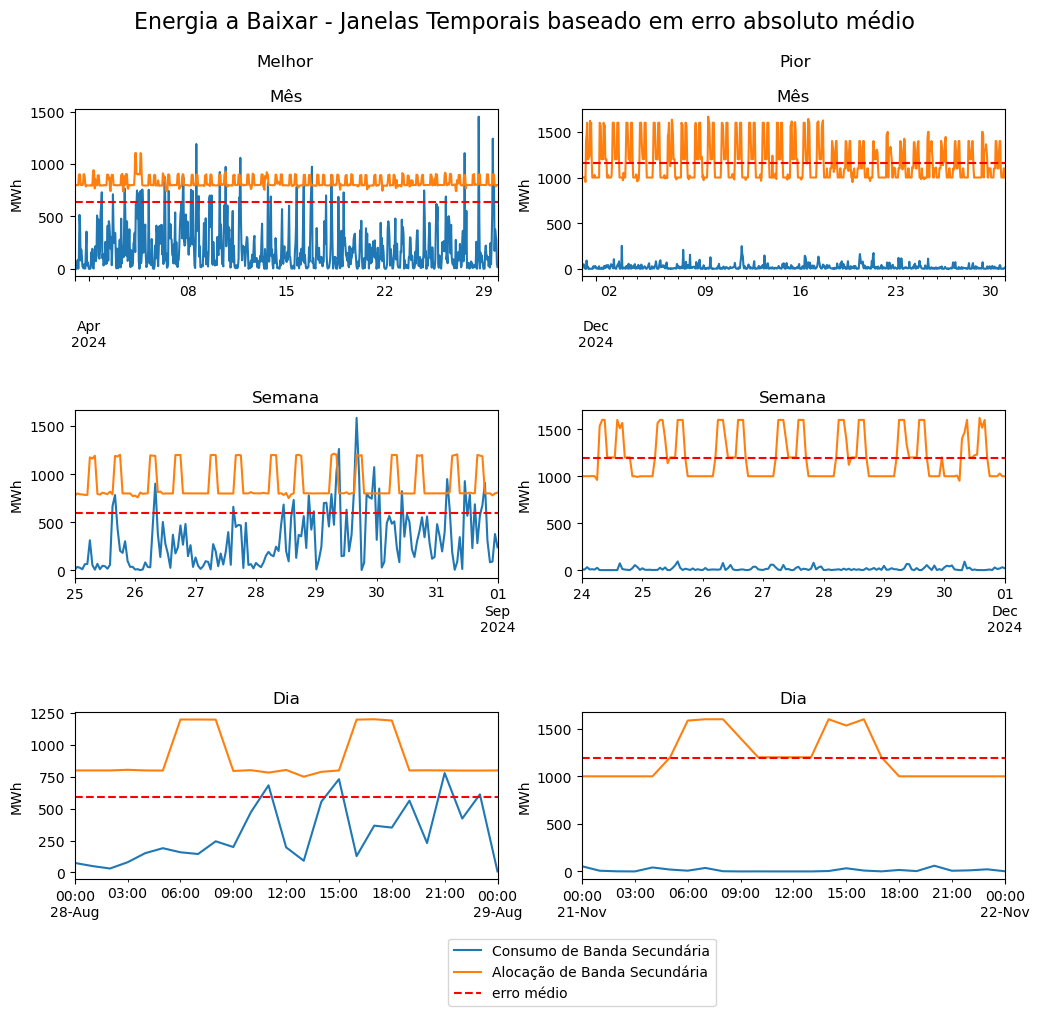
\includegraphics[width=\textwidth]{plots/alocacoes_temporais_downward_dataset.png}
    \caption{Janelas temporais de benchmark energia a descer}
    \label{fig:benchmarktimewindowsdown}
\end{figure}

Dentro destas janelas temporais conseguimos ter melhor a percepção da natureza estática deste modelo actual, e quão longe está dos valores reais necessários.\\

Os resultados a querer melhorar são:\\
\begin{table}[H]
    \caption{Resultados métricas benchmark}    
    \resizebox{\linewidth}{!}{\begin{table}[H] 
    \caption{This is a table caption. Tables should be placed in the main text near to the first time they are~cited.\label{tab1}}
    \newcolumntype{C}{>{\centering\arraybackslash}X}
    \begin{tabularx}{\textwidth}{CCCCC}
    \toprule
    & \textbf{RMSE}	& \textbf{SAE}	& \textbf{AllocF} & \textbf{AllocD}\\
    \midrule
    Up Allocation (MW) & 536.55 & 17357826.75 & 152679.00 & 17205147.75 \\
    Down Allocation (MW) & 408.99 & 12981575.55 & 479191.60 & 12502383.95 \\
        \bottomrule
    \end{tabularx}
    % \noindent{\footnotesize{\textsuperscript{1} Tables may have a footer.}}
\end{table}

}
    \label{tab:benchmarkmetrics}
    \end{table}

As correlações entre o método actual e a energia consumida podem ser vistas na figura abaixo:\\


\begin{figure}[H]
    \centering
    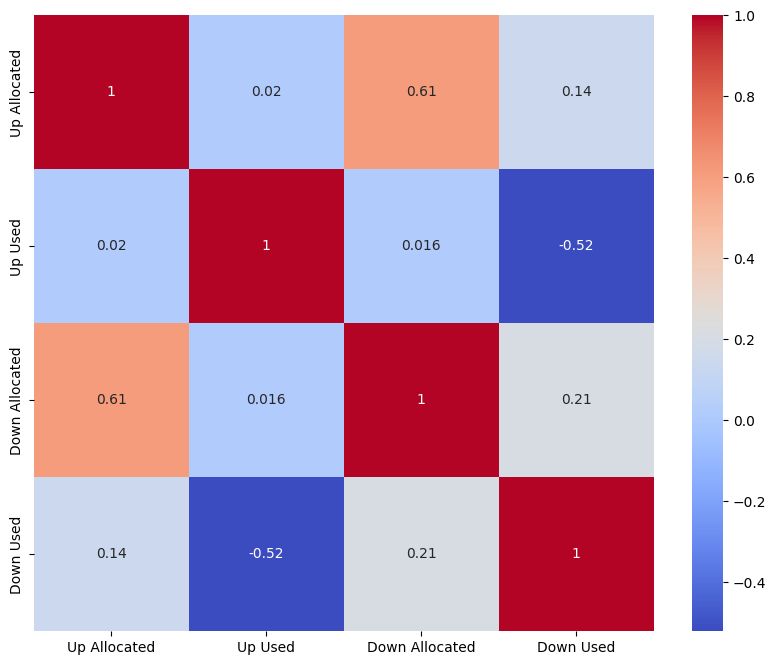
\includegraphics[width=\textwidth]{plots/correlation_heatmap_benchmark.png}
    \caption{Correlação entre benchmark e real}
    \label{fig:benchmarkcorr}
\end{figure}

% TODO: meter formula da previsão ENTO-e no capitulo estudo 2
As relações entres as energias alocadas são altas devido à natureza do \hyperref[]{método de previsão} enqanto que a correlação entre a energia alocada e a usada são bastante baixas com 21\% na alocaçao a descer e 2\% na alocação a subir.\\
O que não mostra uma ligaçao entre as alocações e a energia usada, mas apenas entre as energias alocadas.\\




% Neste capitulo percorremos as experiências realizadas. Estas foram feitas atraves do usos do programas criados para o efeito, disponiveis no repositorio GitHub do \href{https://github.com/JotaFan/renewable-generation-into-reserve-markets}{projecto}.\\

% \section{Benchmark}

% Como modelo benchmark iremos usar a alocação feita. Pois são estes valores que procuramos melhorar no caso prático.\\



% \begin{figure}[H]
%     \centering
%     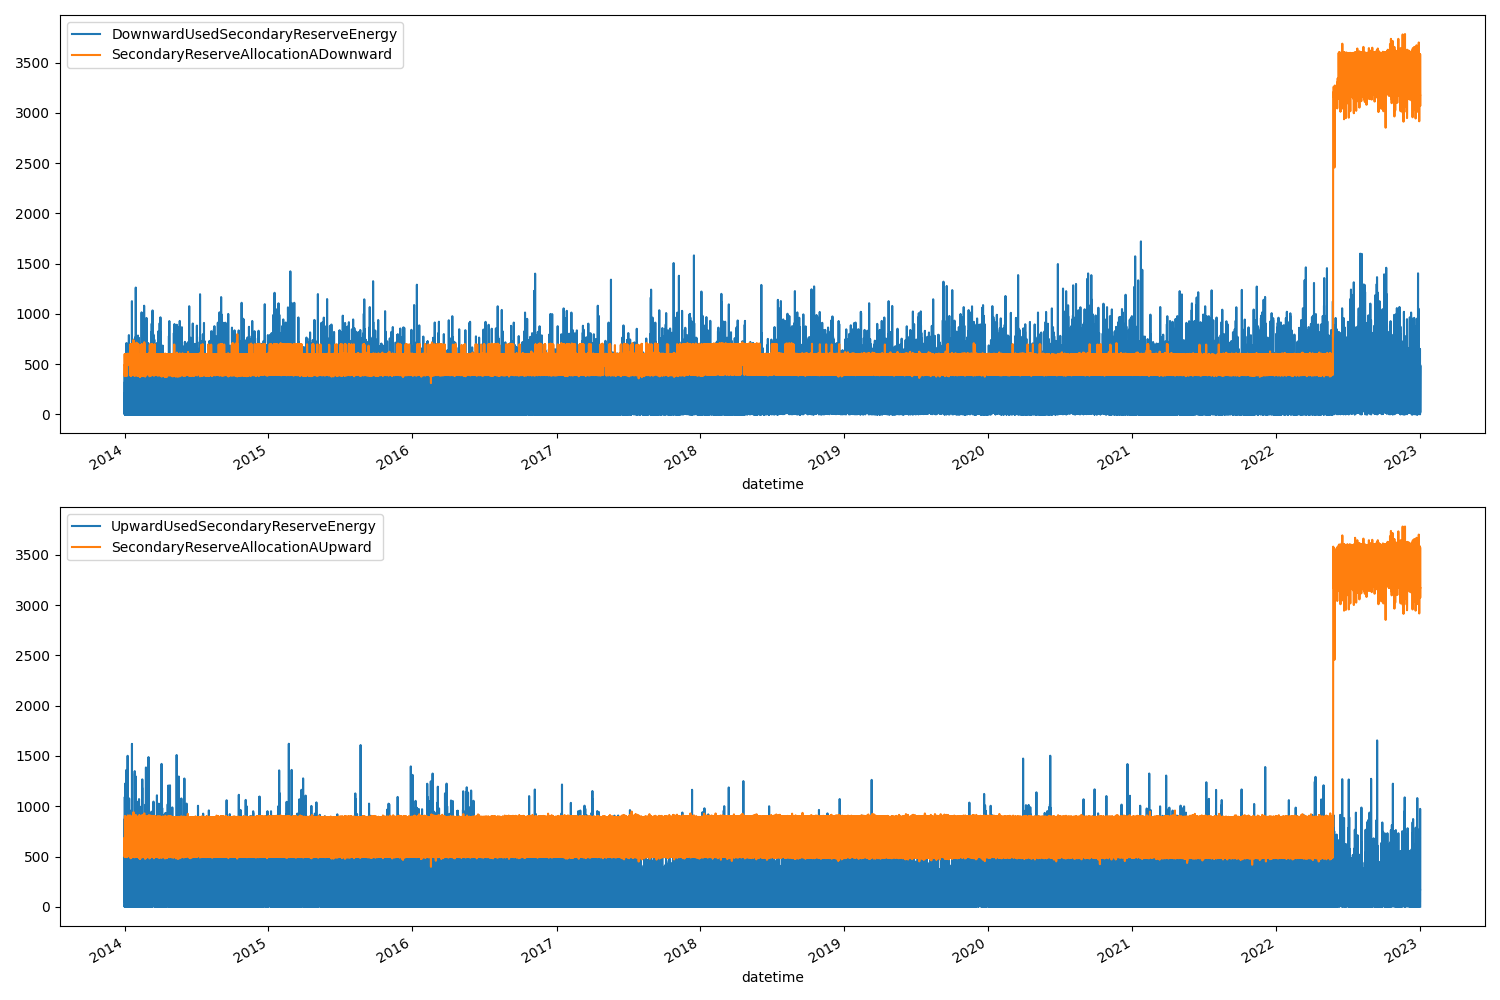
\includegraphics[width=0.8\textwidth]{plots/benchmark.png}
%     \caption{Serie Temporal do benchmark}
%     \label{fig:benchmark}
% \end{figure}
  

% \begin{table}[H]
%     \caption{Dados Benchmark}
%     \resizebox{\linewidth}{!}{\csvautotabular{../data/benchmark_scores.csv}\label{tb:benchmark}}       
% \end{table}


% Para validação dos mesmo, vamos usar o ano 2021, devido aquele salto nos valores de alocação em 2022.\\

% Para esses temos os seguintes dados:

% \begin{figure}[H]
%     \centering
%     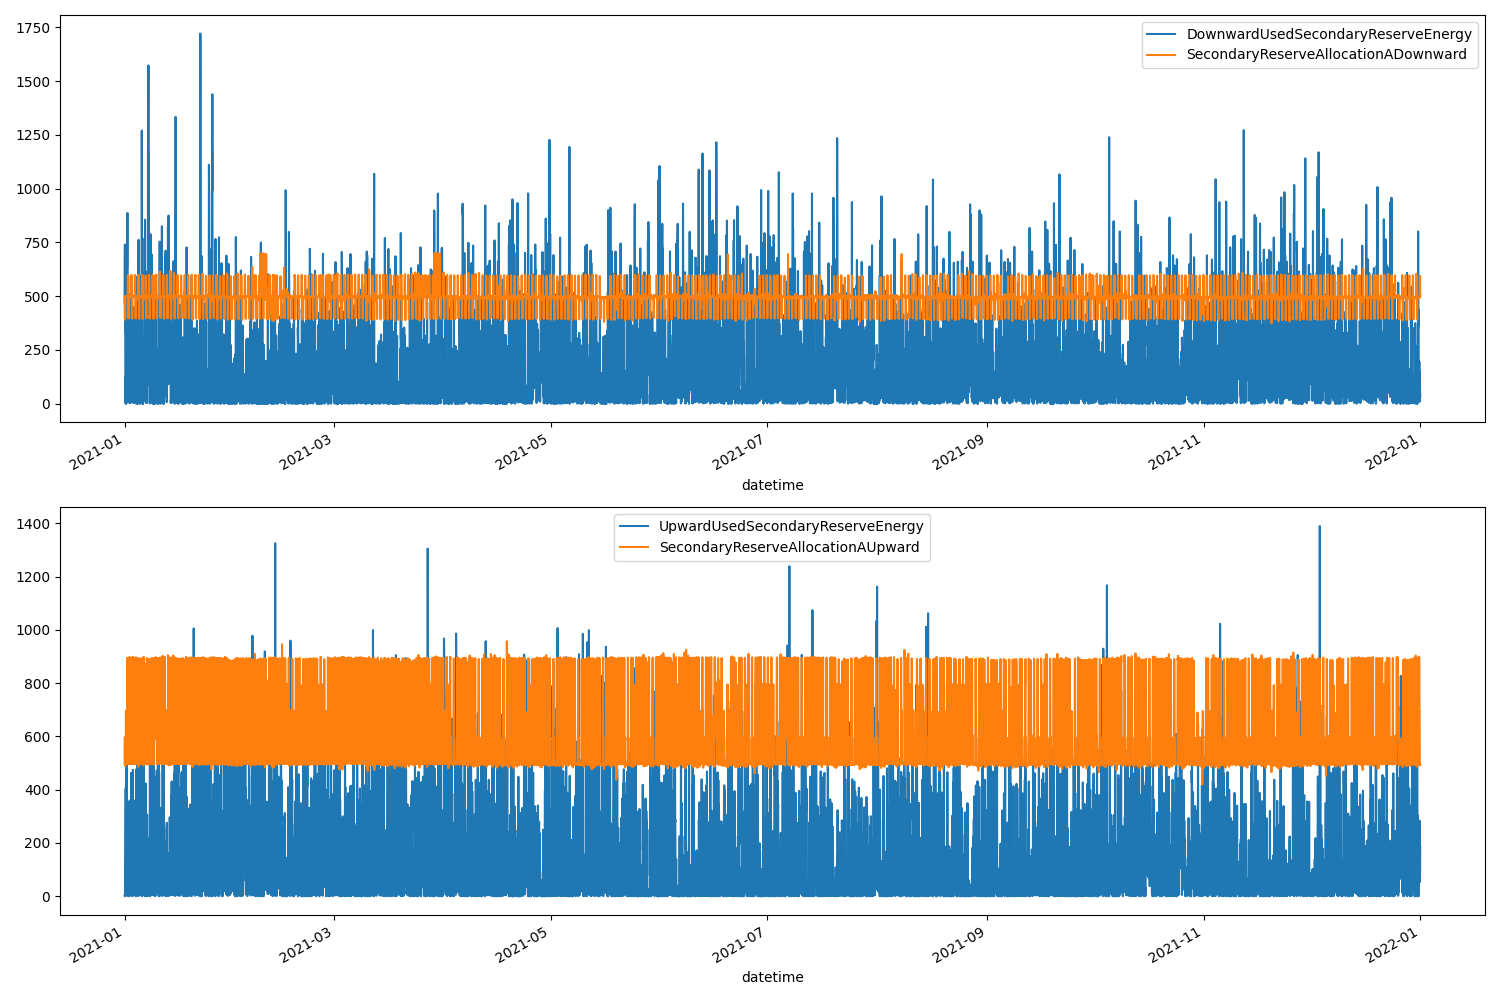
\includegraphics[width=0.8\textwidth]{plots/benchmark_validation.png}
%     \caption{Serie Temporal do benchmark 2021}
%     \label{fig:benchmark_validation}
% \end{figure}
  

% Os metodos em estudo vão ser comparados a esta medida. Sendo que o principal é baixar tanto a alocação perdida, como a alocação a mais. Que se traduzem no erro absoluto.\\

% \begin{table}[H]
%     \caption{Dados Benchmark de validação}
%     \resizebox{\linewidth}{!}{\csvautotabular{../data/benchmark_validation_scores.csv}  \label{tb:benchmark_val}}      
% \end{table}

% \section{Modelos estatiscos\label{se:model_stats}}

% Antes de entrar para o densenvolvimento de modelos vamos usar metódos e modelos abertos para usar comparativamente.\\

% Os modelos estatiscos recurrentes em previsões são AR, MA, ARMA, ARIMA, SARIMA para previsões so com um atributo, e para multiplos atributos VAR.\\
% O modelo AR e o VAR não obtiveram resultados aplicaveis, logo foram desconsiderado.\\

% \subsection{Univariate Analysis}

% Estas análises apenas aplicam uma formula à variavel em questão.

% \subsubsection{AR}
% \begin{equation} \label{eq:AR} 
%     y_t = \beta_0 + \beta_1 y_{t-1} + \dots + \beta_p y_{t-p} + \epsilon_t 
% \end{equation}
% onde:
% \begin{itemize}
%   \item $y_t$: O valor da serie no tempo $t$.
%   \item $p$: O número de atrasos.
%   \item $\epsilon_t$: O barulho no tempo $t$.
%   \item $\beta$: O coeficiente dos valores em atrasdo.
% \end{itemize}

% \subsubsection{MA}
% MA - Moving Average

% A MA 


% \begin{equation} \label{eq:MA} 
%     y_t = c + \epsilon_t + \theta_1 \epsilon_{t-1} + \dots + \theta_q \epsilon_{t-q}
% \end{equation}

% \begin{figure}[H]
%     \centering
%     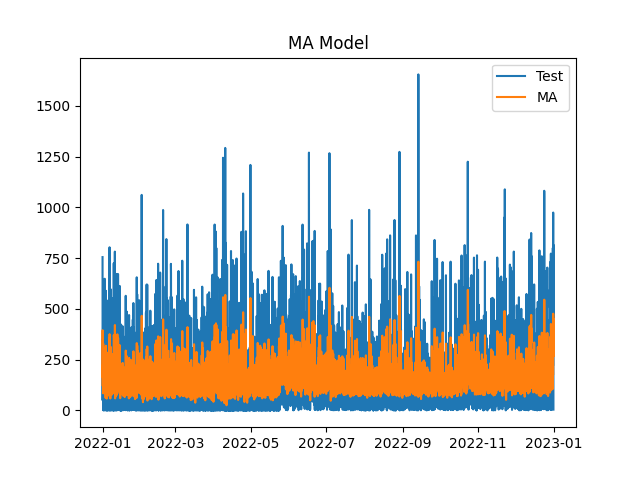
\includegraphics[width=0.8\textwidth]{plots/MA_model.png}
%     \caption{Previsões 2021 com modelo MA}
%     \label{fig:MA_model}
% \end{figure}
  
% \subsection{ARMA}

% AR eé blabla

% \begin{equation} \label{eq:ARMA}  y_t = \beta_0 + \beta_1 y_{t-1} + \dots + \beta_p y_{t-p} + \epsilon_t + \theta_1 \epsilon_{t-1} + \dots + \theta_q \epsilon_{t-q}  \end{equation}
% \textbf{ARMA (Autoregressive Moving Average) Model:}
% \begin{itemize}
%   \item{$y_t$: The value of the time series at time $t$.}
%   \item $p$: The number of time lags to regress on (AR part).
%   \item $q$: The number of time lags of the error term to regress on (MA part).
%   \item $\epsilon_t$: The error term at time $t$.
%   \item $\beta$: The coefficients of the lagged values (AR part).
%   \item $\theta$: The coefficients of the lagged error terms (MA part).
% \end{itemize}


% \begin{figure}[H]
%     \centering
%     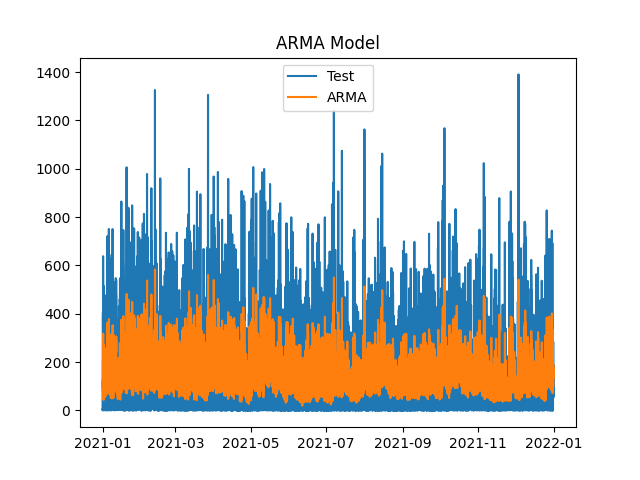
\includegraphics[width=0.8\textwidth]{plots/ARMA_model.png}
%     \caption{Previsões 2021 com modelo ARMA}
%     \label{fig:ARMA_model}
% \end{figure}

% \subsection{ARIMA}

% AR eé blabla

% \begin{equation} \label{eq:ARIMA}y_t^d = \beta_0 + \beta_1 y_{t-1}^d + \dots + \beta_p y_{t-p}^d + \epsilon_t^d + \theta_1 \epsilon_{t-1}^d + \dots + \theta_q \epsilon_{t-q}^d \end{equation}
% \textbf{ARIMA (Autoregressive Integrated Moving Average) Model:}
% \begin{itemize}
%   \item $y_t^{[d]}$: The differenced value of the time series at time $t$.
%   \item $p$: The number of time lags to regress on (AR part).
%   \item $d$: The order of differencing.
%   \item $q$: The number of time lags of the error term to regress on (MA part).
%   \item $\epsilon_t^{[d]}$: The differenced error term at time $t$.
%   \item $\beta$: The coefficients of the lagged values (AR part).
%   \item $\theta$: The coefficients of the lagged error terms (MA part).
% \end{itemize}

% \begin{figure}[H]
%     \centering
%     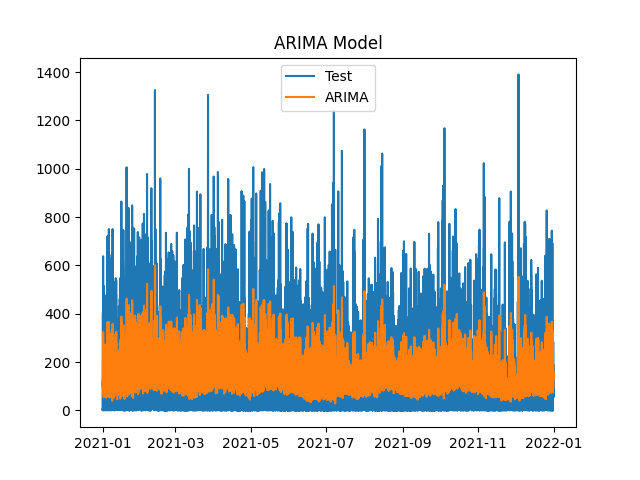
\includegraphics[width=0.8\textwidth]{plots/ARIMA_model.png}
%     \caption{Previsões 2021 com modelo ARIMA}
%     \label{fig:ARIMA_model}
% \end{figure}

% \subsection{SARIMA}

% AR eé blabla



% AR eé blabla

% \begin{equation} \label{eq:SARIMA} y_t^{[m]d} = \beta_0 + \beta_1 y_{t-m}^{[m]d} + \dots + \beta_p y_{t-pm}^{[m]d} + \epsilon_t^{[m]d} + \theta_1 \epsilon_{t-m}^{[m]d} + \dots + \theta_q \epsilon_{t-qm}^{[m]d} \end{equation}

% \textbf{SARIMA (Seasonal Autoregressive Integrated Moving Average) Model:}
% \begin{itemize}
%   \item $y_t^{[m]d}$: The differenced value of the time series at time $t$.
%   \item $p$: The number of time lags to regress on (AR part).
%   \item $d$: The order of differencing.
%   \item $q$: The number of time lags of the error term to regress on (MA part).
%   \item $m$: The number of time lags comprising one full period of seasonality.
%   \item $\epsilon_t^{[m]d}$: The differenced error term at time $t$.
%   \item $\beta$: The coefficients of the lagged values (AR part).
%   \item $\theta$: The coefficients of the lagged error terms (MA part).
% \end{itemize}

% \begin{figure}[H]
%     \centering
%     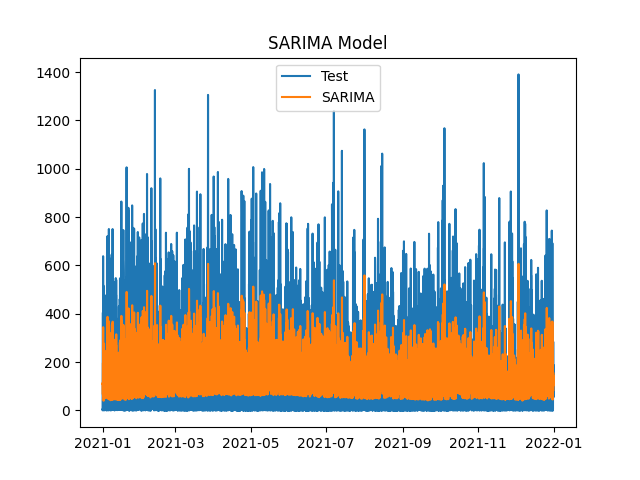
\includegraphics[width=0.8\textwidth]{plots/SARIMA_model.png}
%     \caption{Previsões 2021 com modelo SARIMA}
%     \label{fig:SARIMA_model}
% \end{figure}


% \begin{figure}[H]
%     \centering
%     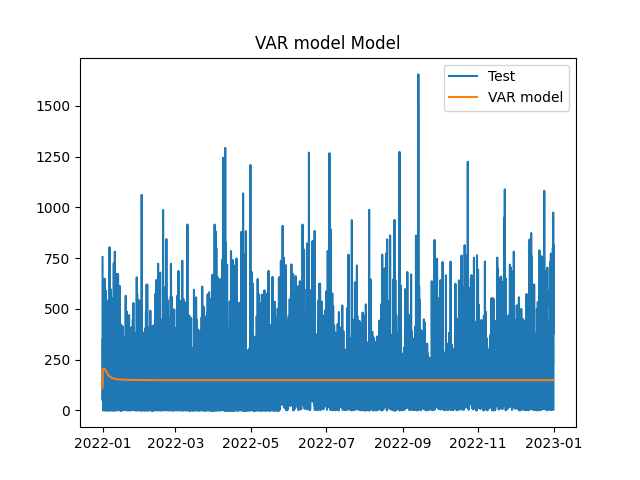
\includegraphics[width=0.8\textwidth]{plots/VAR model_model.png}
%     \caption{Previsões 2021 com modelo VAR}
%     \label{fig:VAR_model}
% \end{figure}









% \subsection{Resultados\label{se:statitics_scores}}

% \begin{table}[H]
%     \caption{Resultados modelos Estatísticos}
%     \resizebox{\linewidth}{!}{\begin{tabular}{llllllllll}
\toprule
rmse & abs erro & erro comp & r2 score & mape score & alloc missing & alloc surplus & optimal percentage & better allocation & beter percentage \\
\midrule
NaN & 0.00 & True & -0.65 & NaN & NaN & NaN & 0.00 & 0.00 & 0.00 \\
171.14 & 1123214.13 & True & 0.14 & 17.04 & 560507.02 & 562707.11 & 63.79 & 63.79 & 86.84 \\
169.99 & 1108555.94 & True & 0.15 & 16.36 & 554443.34 & 554112.60 & 64.04 & 64.04 & 87.17 \\
170.13 & 1111215.12 & True & 0.15 & 16.52 & 556281.62 & 554933.50 & 64.03 & 64.03 & 87.01 \\
171.88 & 1115725.36 & True & 0.13 & 16.43 & 568538.03 & 547187.33 & 63.45 & 63.45 & 86.92 \\
184.60 & 1253196.02 & True & -0.00 & 21.63 & 619929.79 & 633266.23 & 64.82 & 64.82 & 86.07 \\
\bottomrule
\end{tabular}
\label{tb:statitics_scores}}      
% \end{table}

% Apenas pelos métodos estatisticos verificamos que no ano de 2021 teria havido uma melhoria de cerca de 80\% das vezes, usando qualquer um dos métodos apresentados.\\
% Embora a alocação em falta seja de uma ordem de grandeza superior.\\


% \section{Treino e Resultados\label{se:training}}

% Realizaram-se várias experiências, onde em cada um se ia elimando alguns dos objectos em estudo.\\
% Em casa experiências toda a parametrização era igual, à excepção do objecto de estudo.\\

% \subsection{Arquiteturas e numeros de epocas}

% Nesta experiência foi testado o resultado das várias arquiteturas em estudo, como também o impacto do número de epocas na qualidade dos modelos.\\
% As arquitecturas estudadas foram:

% %TODO: arranjar reseach para cada uma 

% \begin{itemize}
%     \item[--] VanillaDense
%     \item[--] VanillaCNN
%     \item[--] VanillaLSTM
%     \item[--] StackedCNN
%     \item[--] StackedLSTM
%     \item[--] EncoderDecoder
%     \item[--] UNET
% \end{itemize}

% O modelos foram treinados em 200 epocas, sendo que foram salvos a cada 10 epocas, de forma conseguirmos perceber os contextos nos saltos de epocas.\\

% As parametrizações usadas:
% \begin{itemize}
%     \item[--] loss : mean squared error
%     \item[--] Metodo activação no meio : relu
%     \item[--] Metodo activação no fim : relu
%     \item[--] optimizador : Adam
%     \item[--] Janela temporal em X : 168 horas (1 semana)
%     \item[--] Janela temporal em Y : 24 horas (1 semana)
%     \item[--] Fracção de treino : 95\%  
% \end{itemize}

% \subsection{Funções de Perda (Loss)}

% TODO: o que é a loss function?

% Esta experiência consiste em rever que função de perda é melhor aplicavel ao problema. Sendo um problema de regressao linear, de valores bastante oscilatórios e com uma distribuição exponencial, temos algumas loss functions que já são reconhecidas para o problema.\\



% \begin{itemize}
%     \item[--] mean absolute error
%     \item[--] mean squared error    
%     \item[--] loss : mean absolute error

% \end{itemize}



% \subsection{Hiperparametrização}

% \subsubsection{Activação}

% \subsubsection{Optimizadores}

% \subsection{Janelas Temporais}

% Um dos pontos deste trabalho é perceber a fesiabilidade de usar dados de previsão do dia anterior (DA) para estes atributos energéticos.\\
% Algo que pode ser também aplicado no futuro a outros dados que não DA, mas sim a 3 horas, ou a 8 horas.\\
% Para perceber esta flexibilidade, mas especialmente para escolher as melhores janelas temporais a usar neste modelos, vamos testar várias combinações.\\
% Mantendo em mente que o objectivo é prever 24 horas, para os casos onde o alvo não dá um previsão de 24 horas, é necessario criar um número de modelos para fazer as 24 horas.\\
% Para validação apenas é usado o espaço temporar previsto, e não multiplos modelos.\\
% Dado as análises de autocorrelação iremos usar como janelas para treino o conjunto [24, 48, 98, 168] para prever o conjunto [1, 4, 8, 12, 24]\\
% Para alem destes foram também testadas combinações com janelas de treino 8 e 12 horas. Estas mostraram rapidamente que janelas de treino menores que as de previsão funcionam muito mal.\\

% \subsection{Classificação}

% Como descrito em (ref)... existe também o uso de tanto classes como valores linears para resolução de problemas de regressão, também chamado \textit{cluster-wise regression}.\\
% Para este teste mudamos um pouco o modelo em uso. Ao invés de apenas uma camada interpretativa, fazemos duas, em paralelo, sendo que uma resolve a regressão e a outra a classificação.\\
% Outro caso, proposto aqui, é usar uma nova camada interpretativa, que combina as duas saidas anteriores (linear e classificação), e resolve novamente para os valores lineares.\\
% Estes modelos não teram apenas uma saida, mas varias, como as arquiteturas MultiTail, mas neste caso cada uma resolve para um problema diferente, com funções de perda, e activações diferentes.\\

% TODO: desenho destas duas camadas intrepretaticas

% \subsection{Pesos}

% Por ultimo foi testado o impacto do uso de pesos nos modelos. Estes pesos são o peso que aquele alvo TODO: epxlicar pesos

% \subsubsection{Modelos lineares}

% Para os modelos lineares o peso que é adiciona ao modelo é a distância à média.\\
% Este peso serve para dar mais importância a valores facilmente considerados outliers.\\



% \subsubsection{Modelos Lineares e de Classificação}
% Aqui o peso é dado por saida. Para as saidas lineares o peso dados é o mesmo que apresentado anteriormente, para a saida de classificação, o peso é o inverso da frequência da classe.\\
% Distribuindo assim a importância de treino pela frquência das classes. Sendo um prática comum especialmente quando as distribuiçoes são muito desiguais, como o caso em estudo.\\
% É aqui estudada a aplicação destes pesos individualmente, e em conjunto. \\
% Os pesos aqui são também normalizados de modo a que o maior peso em cada um deles seja 1, e logo a multiplicação dos dois esteja dentro das mesmas dimensões de relevância.\\


% \begin{equation} \label{eq:peso_media} 
%     P_m = \left| y - mean \right| 
% \end{equation}

% \section{Considerações adicionais  \label{se:metodos_plus}}

% Foram realizados testes adicionais que não obtiveram resultados passivos de boa interpretação, e foram imediatamente descartados, como:

% \begin{itemize}
%     \item[--] Janela temporal em X : 96, 48, 24
%     \item[--] optimizador : todos os optimizadores disponiveis na biblioteca keras
%     \item[--] loss : todas as outra loss functions de regressão disponiveis.
%     \item[--] epocas : influência do número de epocas nos modelos, foram treinados até 20000 epocas alguns modelos mas à medida que a perda ia estagnando na assintomta, o modelo ia apenas piorando.
% \end{itemize}


% Todos os metodos foram realizados utilizando código em python, que está aberto em https://github.com/JotaFan/renewable-generation-into-reserve-markets
\label{ch:metodos}
% Resultados e discussão
\newpage
\thispagestyle{plain}
\chapter{Resultados e discussão}

Os resultados do trabalho conseguem apresentar uma melhoria significativa ao benchmark. Apenas olhando para as flutuações do mesmo já é de esperar uma melhor capacidade de emular os dinamismo do mercado em estudo.\\

\begin{figure}[H]
    \centering
    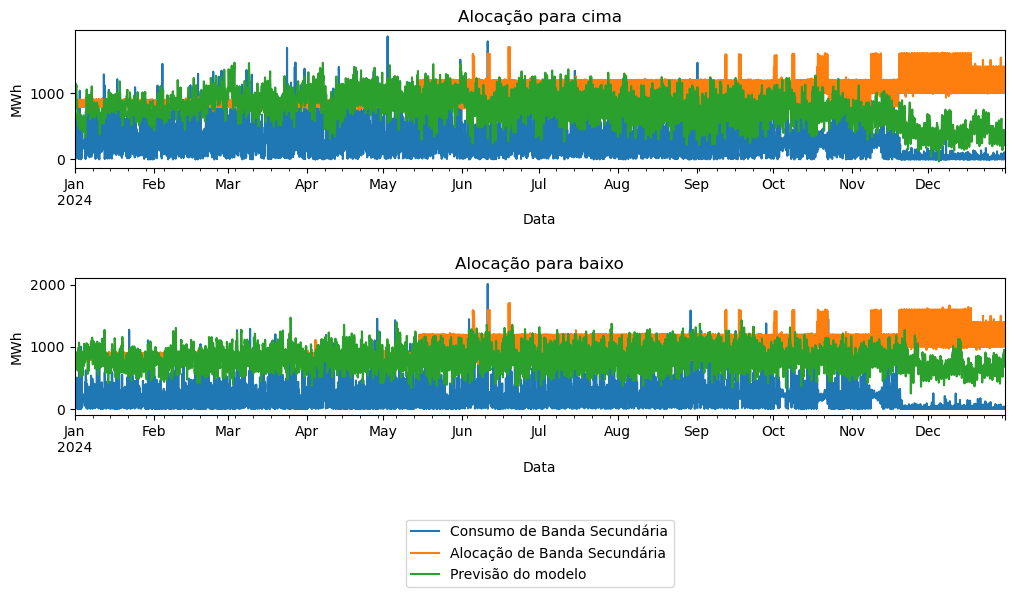
\includegraphics[width=\textwidth]{plots/alocacoes_finais.png}
    \caption{Série Temporal dos dados de validação}
    \label{fig:modeltimeseries}
\end{figure}

Esta figura apresenta os modelos finais durante toda a época de validação. nas secções seguintes vemos ao pormenor os resultados mais importantes de cada experiência.\\

\thispagestyle{plain}
\section{Estatísticos \label{se:resstats}}
Como ponto inicial de resultados os modelos estatísticos apresentam melhorias em relação à alocação em demasia, mas perdas significativas em relação a alocação em falta.\par

\begin{table}[H]
    \caption{Resultados métricas Modelos Estatísticos}    
    \resizebox{\linewidth}{!}{\begin{tabular}{llrrrrrrrrr}
\toprule
 &  & RMSE & SAE & AllocF & AllocD & GPD & GPD F & GPD D & GPD norm & GPD Positivo \\
 & Arquitetura &  &  &  &  &  &  &  &  &  \\
\midrule
\multirow[t]{3}{*}{Alocação a Subir} & ar & 169.21 & 4352584.52 & 2136545.80 & 2216038.73 & 74.92 & -1299.37 & 87.12 & -606.13 & 0.00 \\
 & arma & 181.33 & 4783841.06 & 2187173.52 & 2596667.54 & 72.44 & -1332.53 & 84.91 & -623.81 & 0.00 \\
 & ma & 183.10 & 4940770.16 & 2066116.05 & 2874654.11 & 71.54 & -1253.24 & 83.29 & -584.97 & 0.00 \\
\cline{1-11}
\multirow[t]{3}{*}{Alocação a Descer} & ar & 198.75 & 5265558.19 & 2624914.00 & 2640644.18 & 59.44 & -447.78 & 78.88 & -184.45 & 0.00 \\
 & arma & 218.76 & 5847476.54 & 2876213.76 & 2971262.78 & 54.96 & -500.22 & 76.23 & -211.99 & 0.00 \\
 & ma & 217.53 & 5869239.18 & 2871295.12 & 2997944.06 & 54.79 & -499.20 & 76.02 & -211.59 & 0.00 \\
\cline{1-11}
\bottomrule
\end{tabular}
}
    \label{tab:statsmetrics}
    \end{table}

Estes valores, a nível operacional, podem ser equiparáveis a alocar pouca ou nenhuma energia. Não correndo riscos de alocar em demasia. O que melhora bastante o desempenho em relação ao benchmark a nível de valor de energia absoluta desperdiçada mas derrota o propósito das reservas de energia.\par

\begin{figure}[H]
    \centering
    \includegraphics[width=\textwidth]{plots/alocacoes_temporais_upward_prediction_gpd_stats.png}
    \caption{Janelas temporais de modelos estatísticos energia a subir}
    \label{fig:statstimewindowsup}
\end{figure}


\begin{figure}[H]
    \centering
    \includegraphics[width=\textwidth]{plots/alocacoes_temporais_downward_prediction_gpd_stats.png}
    \caption{Janelas temporais de modelos estatísticos energia a descer}
    \label{fig:statstimewindowsdown}
\end{figure}

Estas figuras mostram que os modelos conseguem até acompanhar o real, podendo até ser um caminho a seguir com algum trabalho específico, mas perdem por manterem-se quase sempre abaixo do necessário, não dando assim a operacionalidade necessária à rede.\par
As médias horárias são:\\
\begin{table}[H]
    \resizebox{\linewidth}{!}{\begin{tabular}{llllll}
\toprule
 &  & média & desvio padrão & min & max \\
\midrule
\multirow[t]{2}{*}{Alocação a Descer (MW)} & benchmark & 542.59 & 126.09 & 363.00 & 946.00 \\
 & modelo & 200.14 & 103.62 & 0.00 & 915.37 \\
\cline{1-6}
\multirow[t]{2}{*}{Alocação a Subir (MW)} & benchmark & 623.68 & 152.39 & 419.00 & 958.00 \\
 & modelo & 160.49 & 77.05 & 0.00 & 765.82 \\
\cline{1-6}
\multirow[t]{2}{*}{Capacidade Horária (MW)} & benchmark & 1166.27 & 250.19 & 816.00 & 1891.00 \\
 & modelo & 360.63 & 109.25 & 45.53 & 1039.76 \\
\cline{1-6}
\multirow[t]{2}{*}{Energia a Descer Extraordinária (MWh)} & benchmark & 169.93 & 153.95 & 0.10 & 1226.40 \\
 & modelo & 192.13 & 168.57 & 0.00 & 1481.53 \\
\cline{1-6}
\multirow[t]{2}{*}{Energia a Subir Extraordinária (MWh)} & benchmark & 139.31 & 136.45 & 0.40 & 922.80 \\
 & modelo & 180.43 & 164.43 & 0.01 & 1508.90 \\
\cline{1-6}
\bottomrule
\end{tabular}
}
    \caption{Resultados Modelos Estatísticos}
    \label{tab:statsres}
    \end{table}



\begin{table}[H]
    \resizebox{\linewidth}{!}{\begin{tabular}{rrrrr}
\toprule
Alocação a Descer & Alocação a Subir & Capacidade Horária & Energia a Descer Extraordinária & Energia a Subir Extraordinária \\
\midrule
-63.11 & -74.28 & -69.08 & 13.06 & 29.65 \\
\bottomrule
\end{tabular}
}
    \caption{$\Delta$\% das médias dos Modelos Estatísticos}    
    \label{tab:statsres_deltas}
    \end{table}

As médias de alocação são bem mais baixas que o benchmark, mas este modelos têm bastante falta de energia alocada em ambas, logo não respondem à premissa base de ter menos energia em falta e em demasia, inclusivo têm um aumento de necessidade de uso de reserva terciária.\par


\thispagestyle{plain}
\subsection{Redes Neuronais \label{se:resml}}

Os vários métodos percorreram muitos tipos de modelos diferentes. Na tabela seguinte apresentamos apenas os melhores resultados baseados em GPD Positivo\par


\begin{table}[H]
    \caption{Resultados métricas Modelos Neuronais}    
    \resizebox{\linewidth}{!}{\begin{tabular}{llrrrrrrrrr}
\toprule
 &  & RMSE & SAE & AllocF & AllocD & GPD & GPD F & GPD D & GPD norm & GPD Positivo \\
 & Arquitetura &  &  &  &  &  &  &  &  &  \\
\midrule
\multirow[t]{5}{*}{Alocação a Subir} & UNET200 & 317.86 & 9759154.87 & 151181.25 & 9607973.62 & 43.78 & 0.98 & 44.16 & 22.57 & 43.78 \\
 & VanillaCNN200 & 328.88 & 10208138.49 & 147549.10 & 10060589.40 & 41.19 & 3.36 & 41.53 & 22.44 & 41.19 \\
 & UNET & 349.91 & 11008787.25 & 146742.39 & 10862044.86 & 36.58 & 3.89 & 36.87 & 20.38 & 36.58 \\
 & VanillaCNN & 370.73 & 11804382.23 & 149719.91 & 11654662.32 & 31.99 & 1.94 & 32.26 & 17.10 & 31.99 \\
 & 2StackedCNN200 & 410.28 & 13223932.55 & 126341.23 & 13097591.32 & 23.82 & 17.25 & 23.87 & 20.56 & 23.82 \\
\cline{1-11}
\multirow[t]{5}{*}{Alocação a Descer} & UNET200 & 282.52 & 8243468.87 & 469060.52 & 7774408.35 & 36.50 & 2.11 & 37.82 & 19.97 & 36.50 \\
 & VanillaCNN200 & 289.59 & 8671975.58 & 476040.73 & 8195934.85 & 33.20 & 0.66 & 34.45 & 17.55 & 33.20 \\
 & UNET & 304.28 & 9172373.23 & 470149.87 & 8702223.36 & 29.34 & 1.89 & 30.40 & 16.14 & 29.34 \\
 & VanillaCNN & 313.42 & 9483287.93 & 475881.60 & 9007406.33 & 26.95 & 0.69 & 27.95 & 14.32 & 26.95 \\
 & VanillaFCNN200 & 344.05 & 10438899.42 & 476740.17 & 9962159.25 & 19.59 & 0.51 & 20.32 & 10.41 & 19.59 \\
\cline{1-11}
\bottomrule
\end{tabular}
}
    \label{tab:mlresmetrics}
    \end{table}

O melhor modelo para alocação a Descer apresenta um ganho de desempenho em relação ao \textit{benchmark} de 42\%, e o a Subir de 47\% na soma da janela temporal de validação.\par
Estes modelos têm ambas as alocações e os erros menores que o \textit{benchmark}. Considerando que os dados que permitem quantificar a mais valia económica de reduzir a alocação de reserva secundária em falta devido não são dados públicos, o objetivo passa por manter esta alocações com valores mais baixos que o \textit{benchmark} (GPDF positivo mas próximo de 0) e minimizar a alocação em excesso, maximizando o GPDD, ou juntando as condições maximizando o GPD Positivo. Desta forma a primeira arquitetura de cada tabela é aquela que apresenta melhores resultados quantificáveis quer do ponto de vista operacional como económico.\par
Escolhendo o modelo com melhores resultados em GPD Positivo podemos ver algumas janelas temporais.\par


\begin{figure}[H]
    \centering
    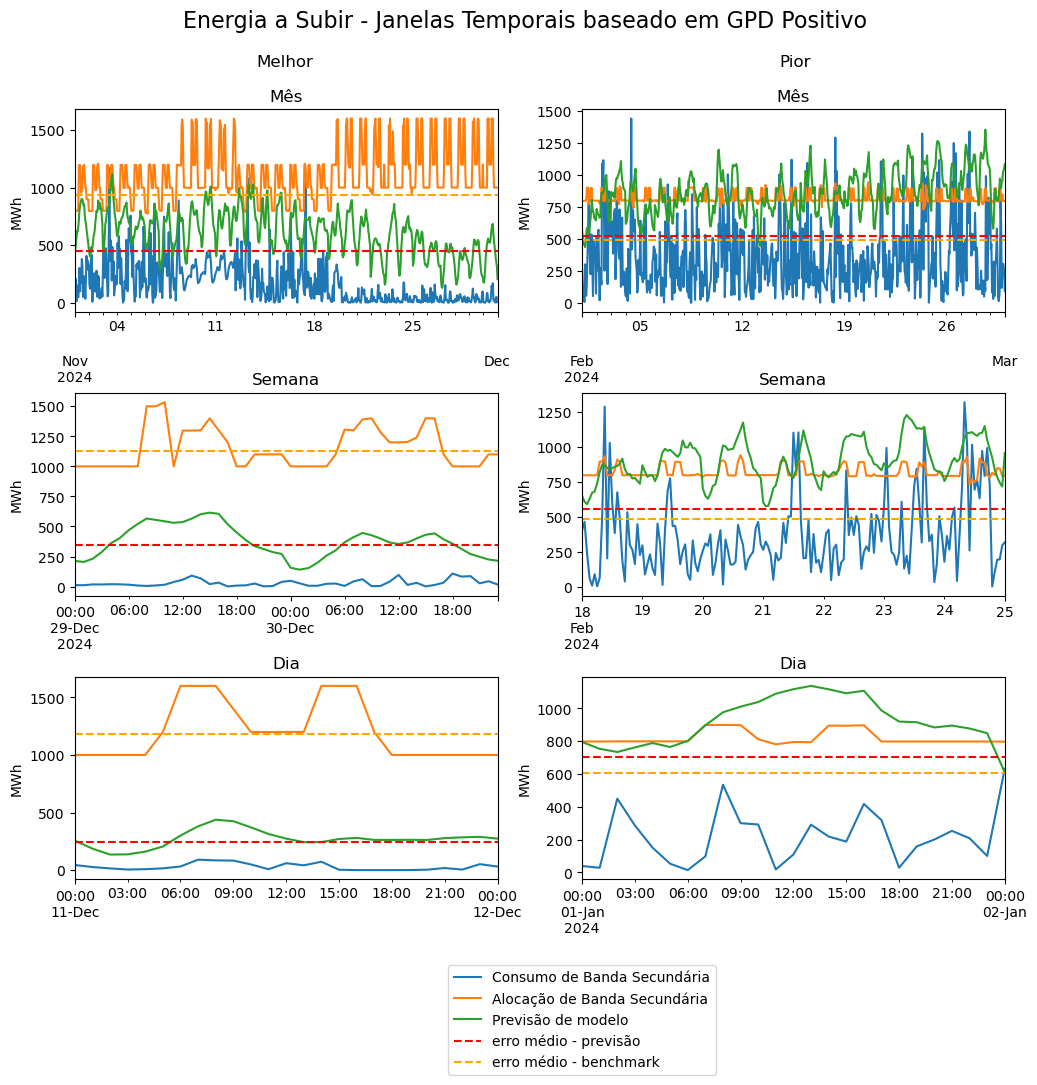
\includegraphics[width=\textwidth]{plots/alocacoes_temporais_upward_prediction_gpd_p.png}
    \caption{Janelas temporais energia a subir}
    \label{fig:mltimewindowsup}
\end{figure}


\begin{figure}[H]
    \centering
    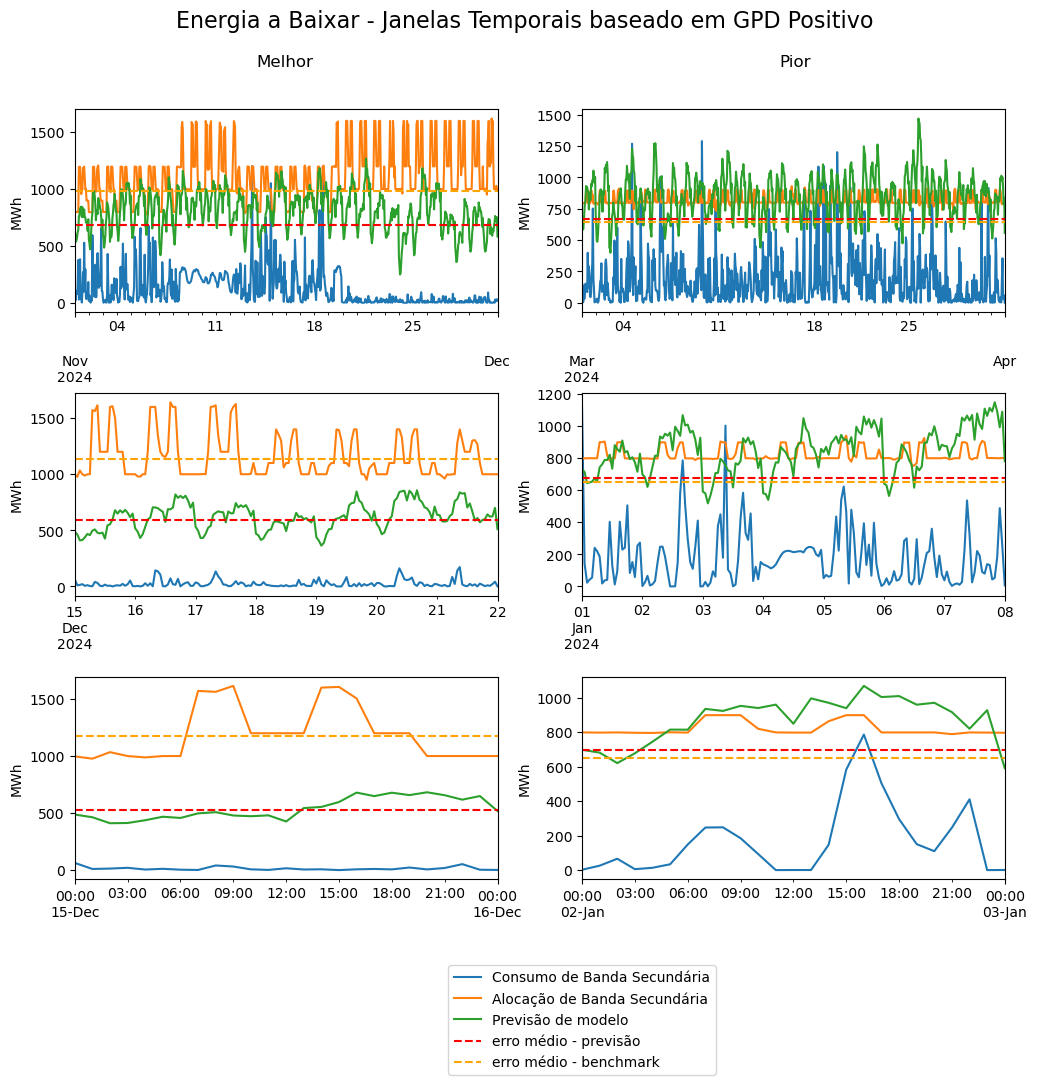
\includegraphics[width=\textwidth]{plots/alocacoes_temporais_downward_prediction_gpd_p.png}
    \caption{Janelas temporais energia a descer}
    \label{fig:mltimewindowsdown}
\end{figure}

É visualmente notável que o modelo mantém uma previsão mais perto da energia usada do que o \textit{benchmark}. Mesmo nas piores janelas temporais, o erro de previsão acumulado é claramente menor que o do método actual.\par
Atente-se no facto de as previsões seguirem bastante mais fielmente as curvas e picos apresentados nos valores de alocação reais, especialmente nas janelas de mês onde temos mais amostras. É possível perceber que o modelo quase sempre acompanha picos da energia usada voltado a baixar quando estes também baixam, destacando-se assim do actual método que mantém uma linha de base bastante mais elevada (desperdiçando mais recursos) e com flutuações que não descrevem tão bem a realidade.\par
Esta flexibilidade no modelo de redes neuronais permite ao operador ter um sinal muito mais flexível diminuindo, deste modo, a alocação desperdiçada.\par

\begin{figure}[H]
    \centering
    \includegraphics[width=\textwidth]{plots/alocation_sum_over_time.png}
    \caption{Soma de Banda Secundária}
    \label{fig:mltimewindowssum}
\end{figure}

Os gráficos anteriores vêm realçar esta mesma ideia. Analisando a energia cumulativa dentro janelas em destaque percebemos que o método proposto mantém quase sempre uma melhoria relativamente ao método utilizado. Esta melhoria é igualmente visível mesmo quando passamos a janelas diárias e semanais, embora haja um aumento considerável das vezes em que o método proposto não é melhor que o actual. E mais importante, o desenho das flutuações é bastante mais fiel ao real.\par


\begin{table}[H]
    \centering
    \caption{Resultados Modelos}    
    \resizebox{0.8\linewidth}{!}{\begin{table}[H] 
    \caption{Model Results and (allocated) values wthin 2024.\label{model_vs_bench}}
    \begin{adjustwidth}{-\extralength}{0cm}
    \newcolumntype{C}{>{\centering\arraybackslash}X}
    \begin{tabularx}{\fulllength}{CCCCCC}
    \toprule
    & & \textbf{mean}	& \textbf{std}	& \textbf{min} & \textbf{max}\\


    \midrule
            \multirow[m]{2}{*}{Down Allocation (MW)}	        & & (921.84) & (191.03) & (720.00) & (1708.00) \\
                                                                & & 836.85 & 182.04 & 247.82 & 1469.62 \\
            \multirow[m]{2}{*}{Up Allocation (MW)}	            & & (921.49) & (191.72) & (719.00) & (1694.00) \\
                                                                & & 778.42 & 228.85 & -29.47 & 1458.01 \\
            \multirow[m]{2}{*}{Hourly Capacity (MW)}	        & & (1843.32) & (382.35) & (1439.00) & (3399.00) \\
                                                                & & 1615.27 & 346.50 & 393.85 & 2594.85 \\
            \multirow[m]{2}{*}{Extraordinary Down Energy (MWh)}	& & (168.74) & (175.69) & (0.90) & (1214.00) \\
                                                                & & 149.66 & 179.96 & 2.66 & 1358.81 \\   
            \multirow[m]{2}{*}{Extraordinary Up Energy (MWh)}	& & (179.39) & (163.94) & (1.00) & (1054.80) \\
                                                                & & 141.85 & 153.57 & 1.83 & 1420.22 \\
    \bottomrule
    \end{tabularx}
    \end{adjustwidth}
\end{table}
}
    \label{tab:mlres}
    \end{table}



\begin{table}[H]
    \caption{$\Delta$\% das médias dos Modelos}    
    \resizebox{\linewidth}{!}{\begin{table}[H] 
    \caption{Mean $\Delta$\% between model and benchmark\label{model_vs_bench_perc}}
    \newcolumntype{C}{>{\centering\arraybackslash}X}
    \begin{tabularx}{\textwidth}{CC}
    \toprule
    & \textbf{$\Delta$\%} \\
    

    \midrule
            Down Allocation (MW)	        & -28.62 \\
            Up Allocation (MW)              & -37.26 \\
            Hourly Capacity (MW)	        & -33.24 \\
            Extraordinary Down Energy (MWh)	& -51.62 \\
            Extraordinary Up Energy (MWh)	& -59.47 \\
    \bottomrule
    \end{tabularx}
    % \noindent{\footnotesize{\textsuperscript{1} Tables may have a footer.}}
\end{table}


}
    \label{tab:mlres_deltas}
    \end{table}

O método proposto apresenta uma melhoria total, durante o período de validação, de \textasciitilde47\% na alocação a subir e \textasciitilde42\% na alocação a descer face ao método usado no mercado. As melhorias médias são de \textasciitilde37\% e \textasciitilde29\% respectivamente, o que também é uma melhoria face ao estado da arte \cite{Algarvio2024} com 13\% e 8\%.\par
O método proposto liberta em média \textasciitilde33\% dos recursos horários, e baixando a necessidade de activar a reserva terciária em \textasciitilde52\% e \textasciitilde59\%.\par

As correlações entre o modelo e a realidade são também mais elevadas que entre \hyperref[fig:featurecorrelation]{modelo e \textit{benchmark}}.


\begin{figure}[H]
    \centering
    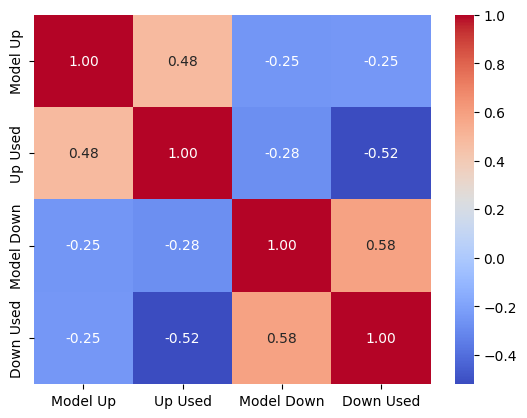
\includegraphics[width=0.8\textwidth]{plots/heatmap_correlation_pred.png}
    \caption{Correlação entre previsão e real}
    \label{fig:predcorrelation}
  \end{figure}

Este mapa de correlações é quase o oposto do apresentado pelo \hyperref[fig:benchmarkcorr]{\textit{benchmark}}.\par
Aqui as correlações maiores são, como seria de esperar, entre a energia usada e a sua alocaçao. Com 48\% na energia a subir e 58\% a descer. E as energias alocadas têm uma correlaçao baixa.\par 
\label{ch:resultados_discussao}
% Conclusões e sugestões futuras
\newpage
\thispagestyle{plain}
\chapter{Conclusões e sugestões futuras}

Primeiramente podemos ver pela análise estatística \ref{tab:statsres} e aplicando a ideia \cite{Elsayed}, simples modelos estatísticos conseguiriam baixar bastante o erro de previsão, melhor do que o que é utilizado actualmente \ref{tab:benchmarkmetrics}, embora tenham aumentado a necessidade de alocação na reserva terciária.\\
E se considerarmos ainda que os modelos estatísticos apresentados que apresentam estes resultados, utilizam apenas a variável em questão, e não todos os outros atributos, a nível de aplicabilidade já são uma melhoria. \\
Em relação a métodos \textit{machine learning}, com poucos recursos computacionais, conseguimos já modelos que superam o método actual.\\
Com modelos relativamente simples conseguimos melhorias muito grandes na alocação de energia, em relação à alocada actualmente. Estes métodos podem criar grandes ganhos financeiros, e diminuir a quantidade de recursos desperdiçados, logo têm um efeito positivo no mercado de reservas.\\
Os resultados aqui apresentados provam que vários tipos de modelos de \textit{machine learning} conseguem realizar previsões bem mais exactas, e que diminuem os recursos usados. Para uso em mercado real estes podem ser adaptados para responder ao mercado em questão, e ao contrário de uma fórmula, podem ir “aprendendo” e melhorando com o passar do tempo.\\
O que mostra que usando estes métodos dinâmicos podemos sim reduzir as incertezas da penetração das \gls{vRES} na alocação de energia secundária.\\
O futuro da indústria pode passar por este tipo de metodologias. Uma maneira de melhorar ainda mais estes resultados seria o uso de outras variáveis para o modelo. Variáveis essas como os dados de reserva primária, dados meteorológicos e principalmente dados não de \gls{DA} mas reais.\\
Um aumento computacional poderia também ter um aumento significativo nas previsões, usando mais quantidade de dados, usando modelos mais pesados e complexos, mais dados históricos, modelações com dados de mercados diferentes com convergência para o mercado necessário.\\
Outra possibilidade pode ser o uso de \textit{machine learning} para a reparametrização de novas fórmulas baseadas nas já existentes e em uso.\\
Vários caminhos e maneiras podem surgir para aplicar o uso de modelos de \textit{machine learning} em alocação dinâmica de reservas, onde operadores diferentes podem ter arquiteturas e modelos completamente diferentes.
\label{ch:conclusao}
% Referências Bibliográficas
\renewcommand{\bibname}{Referências} %comando para rename a BIBLIOGRAFIA para REFERENCIAS
\addcontentsline{toc}{chapter}{\numberline{10}Referências}
\printbibliography

% Referências Bibliográficas
\appendix
\newpage
\thispagestyle{plain}
\chapter{Anexos}


\label{ch:Anexos}

\end{document}
